	%%%%%%%%%%%%%%%%%%%%%%%%%%%%%%%%%%%%%%%%%
% Masters/Doctoral Thesis 
% LaTeX Template
% Version 2.5 (27/8/17)
%
% This template was downloaded from:
% http://www.LaTeXTemplates.com
%
% Version 2.x major modifications by:
% Vel (vel@latextemplates.com)
%
% This template is based on a template by:
% Steve Gunn (http://users.ecs.soton.ac.uk/srg/softwaretools/document/templates/)
% Sunil Patel (http://www.sunilpatel.co.uk/thesis-template/)
%
% Template license:
% CC BY-NC-SA 3.0 (http://creativecommons.org/licenses/by-nc-sa/3.0/)
%
%%%%%%%%%%%%%%%%%%%%%%%%%%%%%%%%%%%%%%%%%

%----------------------------------------------------------------------------------------
%	PACKAGES AND OTHER DOCUMENT CONFIGURATIONS
%----------------------------------------------------------------------------------------

\documentclass[
11pt, % The default document font size, options: 10pt, 11pt, 12pt
%oneside, % Two side (alternating margins) for binding by default, uncomment to switch to one side
english, % ngerman for German
singlespacing, % Single line spacing, alternatives: onehalfspacing or doublespacing
%draft, % Uncomment to enable draft mode (no pictures, no links, overfull hboxes indicated)
%nolistspacing, % If the document is onehalfspacing or doublespacing, uncomment this to set spacing in lists to single
%liststotoc, % Uncomment to add the list of figures/tables/etc to the table of contents
%toctotoc, % Uncomment to add the main table of contents to the table of contents
parskip, % Uncomment to add space between paragraphs
%nohyperref, % Uncomment to not load the hyperref package
headsepline, % Uncomment to get a line under the header
chapterinoneline, % Uncomment to place the chapter title next to the number on one line
%consistentlayout, % Uncomment to change the layout of the declaration, abstract and acknowledgements pages to match the default layout
oneside
]{MastersDoctoralThesis} % The class file specifying the document structure

\usepackage[utf8]{inputenc} % Required for inputting international characters
\usepackage[T1]{fontenc} % Output font encoding for international characters

\usepackage{mathpazo} % Use the Palatino font by default

\usepackage[backend=bibtex,style=vancouver,natbib=true]{biblatex} % Use the bibtex backend with the authoryear citation style (which resembles APA)

\addbibresource{bibliography.bib} % The filename of the bibliography

\usepackage[autostyle=true]{csquotes} % Required to generate language-dependent quotes in the bibliography
\usepackage{courier}
\usepackage{multicol}
\usepackage{amsmath}
\usepackage{array}
\usepackage{listings}
\usepackage{color}
\usepackage{adjustbox} 
\usepackage{longtable}
\usepackage{lscape}
\usepackage{booktabs}
\usepackage{bm}


% Define colors
\definecolor{codegreen}{rgb}{0,0.6,0}
\definecolor{codegray}{rgb}{0.5,0.5,0.5}
\definecolor{codepurple}{rgb}{0.58,0,0.82}
\definecolor{backcolour}{rgb}{0.95,0.95,0.92}

% Setup the style for the Python code
\lstdefinestyle{mystyle}{
	backgroundcolor=\color{backcolour},   
	commentstyle=\color{codegreen},
	keywordstyle=\color{magenta},
	numberstyle=\tiny\color{codegray},
	stringstyle=\color{codepurple},
	basicstyle=\ttfamily\footnotesize,
	breakatwhitespace=false,         
	breaklines=true,                 
	captionpos=b,                    
	keepspaces=true,                 
	numbers=left,                    
	numbersep=5pt,                  
	showspaces=false,                
	showstringspaces=false,
	showtabs=false,                  
	tabsize=2
}

\lstset{style=mystyle}



%----------------------------------------------------------------------------------------
%	MARGIN SETTINGS
%----------------------------------------------------------------------------------------

\geometry{
	paper=a4paper, % Change to letterpaper for US letter
	inner=2.5cm, % Inner margin
	outer=3.8cm, % Outer margin
	bindingoffset=.5cm, % Binding offset
	top=1.5cm, % Top margin
	bottom=1.5cm, % Bottom margin
	%showframe, % Uncomment to show how the type block is set on the page
}

%----------------------------------------------------------------------------------------
%	THESIS INFORMATION
%----------------------------------------------------------------------------------------

\thesistitle{Esports Betting Technology: Machine Learning for Match Prediction and Odds Estimation} % Your thesis title, this is used in the title and abstract, print it elsewhere with \ttitle
\supervisor{Neil \textsc{Watson}} % Your supervisor's name, this is used in the title page, print it elsewhere with \supname
\examiner{} % Your examiner's name, this is not currently used anywhere in the template, print it elsewhere with \examname
\degree{Master of Philosophy specialising in Financial Technology} % Your degree name, this is used in the title page and abstract, print it elsewhere with \degreename
\author{Henri Izak David \textsc{du Plessis}} % Your name, this is used in the title page and abstract, print it elsewhere with \authorname
\addresses{} % Your address, this is not currently used anywhere in the template, print it elsewhere with \addressname

\subject{Statistical Sciences} % Your subject area, this is not currently used anywhere in the template, print it elsewhere with \subjectname
\keywords{} % Keywords for your thesis, this is not currently used anywhere in the template, print it elsewhere with \keywordnames
\university{University of Cape Town} % Your university's name and URL, this is used in the title page and abstract, print it elsewhere with \univname
\department{School of Economics} % Your department's name and URL, this is used in the title page and abstract, print it elsewhere with \deptname
\group{\href{http://researchgroup.university.com}{Research Group Name}} % Your research group's name and URL, this is used in the title page, print it elsewhere with \groupname
\faculty{Faculty of Commerce} % Your faculty's name and URL, this is used in the title page and abstract, print it elsewhere with \facname

\AtBeginDocument{
\hypersetup{pdftitle=\ttitle} % Set the PDF's title to your title
\hypersetup{pdfauthor=\authorname} % Set the PDF's author to your name
\hypersetup{pdfkeywords=\keywordnames} % Set the PDF's keywords to your keywords
}

\begin{document}

\frontmatter % Use roman page numbering style (i, ii, iii, iv...) for the pre-content pages

\pagestyle{plain} % Default to the plain heading style until the thesis style is called for the body content

%----------------------------------------------------------------------------------------
%	TITLE PAGE
%----------------------------------------------------------------------------------------

\begin{titlepage}
\begin{center}

\vspace*{.06\textheight}
{\scshape\LARGE \univname\par}\vspace{1.5cm} % University name
\textsc{\Large Minor Dissertation}\\[0.5cm] % Thesis type

\HRule \\[0.4cm] % Horizontal line
{\huge \bfseries \ttitle\par}\vspace{0.4cm} % Thesis title
\HRule \\[1.5cm] % Horizontal line
 
\begin{minipage}[t]{0.4\textwidth}
\begin{flushleft} \large
\emph{Author:}\\
{\authorname} % Author name
\end{flushleft}
\end{minipage}
\begin{minipage}[t]{0.4\textwidth}
\begin{flushright} \large
\emph{Supervisor:} \\
{\supname} % Supervisor name
\end{flushright}
\end{minipage}\\[3cm]
 
\vfill

\large \textit{A minor dissertation submitted in partial fulfilment of the requirements for the degree of \degreename}\\[0.3cm] % University requirement text
\textit{in the}\\[0.4cm]
\deptname\\[2cm] % Research group name and department name
 
\vfill

{\large \today}\\[4cm] % Date
%\includegraphics{Logo} % University/department logo - uncomment to place it
 
\vfill
\end{center}
\end{titlepage}

%----------------------------------------------------------------------------------------
%	DECLARATION PAGE
%----------------------------------------------------------------------------------------

\begin{declaration}

\begin{enumerate} 
\item I know that plagiarism is wrong. Plagiarism is to use another's work and pretend that it is one’s own.
\item I have used the Vancouver referencing system for citation and referencing.  Each contribution to, and quotation in, this minor dissertation \textit{\enquote{\ttitle}}, from the work(s) of other people has been attributed, and has been cited and referenced.
\item Where I have consulted the published work of others, this is always clearly attributed.
\item Where I have quoted from the work of others, the source is always given. With the exception of such quotations, this minor dissertation is entirely my own work.
\item I have acknowledged all main sources of help.
\item Where the minor dissertation is based on work done by myself jointly with others, I have made clear exactly what was done by others and what I have contributed myself.
\vspace{1cm}
\end{enumerate}
 
\noindent Signed:\\
\rule[0.5em]{25em}{0.5pt} % This prints a line for the signature
 
\end{declaration}

\cleardoublepage

%----------------------------------------------------------------------------------------
%	ABSTRACT PAGE
%----------------------------------------------------------------------------------------

\begin{abstract}
\addchaptertocentry{\abstractname} % Add the abstract to the table of contents

Esports betting is a rapidly growing segment of the online sports betting market. A key feature of this industry is the pricing of betting odds. This study investigated the online sports betting industry, odds compilation, and how machine learning can be used for sports prediction. The techniques used in the literature were then applied to one of the world's foremost esports: Counter-Strike. A substantial dataset of professional match data (n=11271) was collected and used to construct 142 relevant features for match prediction. Several supervised learning models, including random forests, feed-forward neural networks, and XGBoost, were trained to estimate win probabilities for both teams in each match. Betting odds were then calculated using these probabilities and compared to real-world betting odds. 

A notable aspect of the research is the implementation of Microsoft's TrueSkill rating system. It served as both a benchmark and an input feature. Among the models tested, XGBoost showed the best overall performance. The highest match prediction accuracy attained was 62.7\%. It was found that incorporating a large number of statistics did not significantly improve predictive accuracy when compared to models using fewer, more important features. It was also found that LAN matches and best-of-3 map formats are more predictable than their counterparts. Despite the inherent difficulty in Counter-Strike match prediction, the models could generate efficient odds which exhibited strong correlation with real-world odds (up to 85\%). A betting strategy informed by the generated odds was back-tested over a six-month period and shown to be profitable.

This research therefore demonstrates how machine learning models can be used for esports match prediction, with practical applications in the online betting industry.

\end{abstract}

%----------------------------------------------------------------------------------------
%	ACKNOWLEDGEMENTS
%----------------------------------------------------------------------------------------

\begin{acknowledgements}
\addchaptertocentry{\acknowledgementname} % Add the acknowledgements to the table of contents


\topskip0pt
\vspace{20pt}
I would like to thank my supervisor, \supname, for his consistent guidance, feedback, and support over the past year.
\vspace{10pt}

I also want to thank my parents, \textsc{Henry} and \textsc{Janet}, for their love and support throughout my life and academic journey.

\vspace{10pt}

Knowing that you believed in me was a powerful source of motivation.
\vspace*{\fill}
\end{acknowledgements}


%----------------------------------------------------------------------------------------
%	LIST OF CONTENTS/FIGURES/TABLES PAGES
%----------------------------------------------------------------------------------------

\tableofcontents % Prints the main table of contents

\listoffigures % Prints the list of figures

\listoftables % Prints the list of tables

%----------------------------------------------------------------------------------------
%	ABBREVIATIONS
%----------------------------------------------------------------------------------------

\begin{abbreviations}{ll}
	\textbf{ADR} & average damage per round \\
	\textbf{AI} & artificial intelligence \\
	\textbf{AUC} & area under ROC curve \\
	\textbf{API} & application programming interface\\
	\textbf{BO\bm{$x$}} & best-of-$x$ \\
	\textbf{CAGR} & compound annual growth rate \\
	\textbf{CPL} & Cyberathlete Professional League \\
	\textbf{CS}  & Counter-Strike \\
	\textbf{CS:GO} & Counter-Strike: Global Offensive\\
	\textbf{CS2} & Counter-Strike 2\\
	\textbf{CT}  & Counter-Terrorist \\
	\textbf{ESL} & Electronic Sports League \\
	\textbf{FPS} & first-person shooter \\
	\textbf{HP} & health points \\
	\textbf{HTTP} & Hypertext Transfer Protocol\\
	\textbf{HTML} & Hypertext Markup Language \\
	\textbf{IEM} & Intel Extreme Masters \\
	\textbf{IGL} & in-game leader \\
	\textbf{IP} & intellectual property \\
	\textbf{KAST} & kill-assist-survived-traded\\
	\textbf{\bm{$k$}-NN} & $k$-nearest neighbours  \\
	\textbf{LAN} & local area network \\
	\textbf{LR} & logistic regression \\
	\textbf{MAE} & mean absolute error \\
	\textbf{ML} & machine learning\\
	\textbf{MLP} & multilayer perceptron \\
	\textbf{MLB} & Major League Baseball \\
	\textbf{MOBA} & multiplayer online battle arena \\
	\textbf{NBA} & National Basketball Association \\
	\textbf{NFL} & National Football League \\
	\textbf{NHL} & National Hockey League \\
	\textbf{NFTs} & non-fungible tokens \\
	\textbf{NN} & neural network \\
	\textbf{PC}  & personal computer \\
	\textbf{PGL} & Professional Gamers League \\
	\textbf{RD} & ratings deviation \\
	\textbf{RMSE} & root mean square error \\
	\textbf{ROC} & receiver operating characteristic \\
	\textbf{RTS} & real-time strategy \\
	\textbf{T}   & Terrorist \\
	\textbf{US}  & United States \\
\end{abbreviations}

%----------------------------------------------------------------------------------------
%	PHYSICAL CONSTANTS/OTHER DEFINITIONS
%----------------------------------------------------------------------------------------

%\begin{constants}{lr@{${}={}$}l} % The list of physical constants is a three column table
%
%% The \SI{}{} command is provided by the siunitx package, see its documentation for instructions on how to use it
%
%Speed of Light & $c_{0}$ & \SI{2.99792458e8}{\meter\per\second} (exact)\\
%%Constant Name & $Symbol$ & $Constant Value$ with units\\
%
%\end{constants}

%----------------------------------------------------------------------------------------
%	SYMBOLS
%----------------------------------------------------------------------------------------

%\begin{symbols}{lll} % Include a list of Symbols (a three column table)
%
%$a$ & distance & \si{\meter} \\
%$P$ & power & \si{\watt} (\si{\joule\per\second}) \\
%%Symbol & Name & Unit \\
%
%\addlinespace % Gap to separate the Roman symbols from the Greek
%
%$\omega$ & angular frequency & \si{\radian} \\
%
%\end{symbols}

%----------------------------------------------------------------------------------------
%	DEDICATION
%----------------------------------------------------------------------------------------

%\dedicatory{For/Dedicated to/To my\ldots} 

%----------------------------------------------------------------------------------------
%	THESIS CONTENT - CHAPTERS
%----------------------------------------------------------------------------------------

\mainmatter % Begin numeric (1,2,3...) page numbering

\pagestyle{thesis} % Return the page headers back to the "thesis" style

% Include the chapters of the thesis as separate files from the Chapters folder
% Uncomment the lines as you write the chapters

\chapter{Introduction}
\label{Introduction}

%I first want to introduce the idea quickly, similar to an abstract. How online sports betting is a big growth industry, how esports are developing big time, how popular it is for people to bet on these esports matches. Then I want to specify how the algorithms used by sports betting companies are clouded in mystery - it's quite difficult to predict the outcome of sports events, and this is no different with esports. Statistical techniques are required, and the large amount of data genered natively by digital 'sports' make it a natural contender for analysis using machine learning techniques.
%
%• Start with a striking statistic or fact to grab attention about the growth of online sports betting and the popularity of esports. Highlight the mystery and complexity behind the algorithms used by betting companies.

\section{Background and context}

The rapid technological development of the 21st century has ushered in a digital transformation of most industries \cite{wef-tech}. The sports betting industry is no different. Placing a bet on the outcome of a sports match is now only a few quick taps away, as droves of online sports betting companies compete to take your wager. Electronic banking facilitates near instantaneous deposits and withdrawals between the user and the bookmaker, and the slew of odds and other betting options are generated 24/7 by computers running statistical models and complex algorithms. All of these advancements have made betting quicker, easier, and more accessible to an ever-expanding market of bettors \cite{structuresportsbetting}.

In a similar vein, the viability of \textit{electronic sports} relies on the uninterrupted functioning of an ensemble of technologies: complex computer hardware and peripherals providing the physical interfaces for the gameplay, the games themselves being the top layer of a highly-advanced software stack, and the high-speed, low-latency networking infrastructure that connects each player to one another in a virtual arena \cite{proesports-book}. With the sudden rise in popularity of this new form of competition, bookmakers have been quick to capitalise on a new market and offer betting opportunities for the outcomes of esports matches \cite{sizesportsbetting}.
 

\subsection{Online sports betting}
\label{background-bet}

Sports betting is a form of gambling whereby the bettor places a monetary wager on the outcome of one or more sporting events \cite{sportsbettingworld}. If the outcome(s) materialise, the bet is won and the bettor receives the value of their wager multiplied by the odds offered by the bookmaker. The odds for a given event are calculated by odds compilers, who analyse historical data and employ statistical techniques to accurately predict the probabilities of different outcomes \cite{oddscompiler}. The mathematical reciprocal of these probabilities determines the odds. To increase their profitability, bookmakers then decrease the odds slightly for either outcome. This difference between the compiled and offered odds is known as the bookmaker's margin \cite{margin}.

It is not known precisely when the practice of sports betting began, however sources claim that the Greeks would bet on the Ancient Olympic Games. The practice later appeared in Rome, where chariot racing and gladiator battles became the subject of the bets \cite{historybetting}. Betting on horse races was a popular activity in the United Kingdom by the early 18th century, and soon spread throughout the developed world \cite{historybetting-lamb}. By 1890, the United States boasted over 300 legal horse racing tracks, with horse race betting becoming a favourable pastime of the upper class. In the US, the industry was heavily regulated, and outright banned in 1910 \cite{historybetting-gray-1}. Regulations evolved over time, and the first government-sanctioned, brick-and-mortar sportsbook opened in Las Vegas in 1949. These businesses were known as 'Turf Clubs', and accepted bets on a number of professional sports, including the National Football League (NFL), National Hockey League (NHL), Major League Baseball (MLB), and National Basketball Association (NBA) \cite{historybetting-gray-2}.

The era of online sports betting began in 1996, when an Austrian-based sports book used the internet to legally connect sports bettors and bookmakers. On January 17th, 1996, the first online wager was made when Jukka Honkavaara bet \$50 on a football match: the first online sportsbook, Intertops (now known as Everygame), offered 1.04 odds for Tottenham Hotspurs to beat Hereford United. Though Honkavaara's winnings only amounted to a modest \$2, this event was nevertheless significant, as it marked the birth of the online sports betting industry \cite{historyonlinegambling}. 

Although regulations have hampered the industry in the US significantly, by 2023 the global market value of sports betting has grown significantly to 243 billion US dollars \cite{structuresportsbetting}. It currently accounts for over 40\% of global gambling revenue around the world - more than casinos, lotteries, and other forms of gambling \cite{sizesportsbetting}. Much of this growth can be attributed to the digitisation of the industry, which has led to increased access to and availability of betting opportunities. In 2018, the federal ban on sports betting in the US was lifted, and today it has been legalized in most states \cite{legalbettingtracker}. Furthermore, the industry is expected to grow significantly in Asia and Africa as laws surrounding sports betting become more relaxed and access to the online betting platforms improves \cite{structuresportsbetting}. The modern features and mechanics of the online betting industry will be further explored in the next chapter.

\subsection{Electronic sports}

The fastest-growing sports market, in terms of betting volume, are \textit{electronic sports}, also known as esports \cite{sizesportsbetting}. Esports are video games played in a competitive setting \cite{arcade}. The practice started in the 1970s and 80s on the floors of public arcades. The best players would rise to the top of persistent high-score leaderboards in their favourite titles like \textit{Space Invaders}, \textit{Pac-Man}, and \textit{Tetris} \cite{economicsjournalesports}. This type of competition was indirect, but by the 1990s, multi-player fighting games like \textit{Street Fighter} would see players pitted directly against each other. By then, the transition from arcades floors to home consoles and personal computers (PCs) was well under way, and the Local Area Network (LAN) party became the new battle arena. \textit{Doom} and \textit{Quake} marked the rise of first-person shooters (FPS) in this era. At the dawn of the 2000s, real-time strategy (RTS) games like \textit{StarCraft} and \textit{Warcraft} spawned the first professional leagues, legitimizing competitive gaming \cite{koreasports}.

High-speed internet became ubiquitous by the 2010s, and esports went mainstream. Multiplayer online battle arena (MOBA) games like \textit{League of Legends} and \textit{Dota 2} rose to prominence, and now boast tournaments with multi-million dollar prize pools. The largest esports prize pool to date was \textit{The International 2021} in Bucharest, Romania, with \$40 million US being awarded to the competitors \cite{growthofesports}. Although most are team games, some esports entail single players competing against one or more other players. In \textit{Fortnite}, only one player can emerge victorious in a 100-player 'battle royale', where the last surviving player wins. Kyle Giersdorf won at the Fortnite World Cup Finals 2019 at the age of 16, winning \$3 million US in the process. 

Today there are a substantial variety of game genres that are played professionally across the globe. Viewership figures for the major tournaments already rival traditional sports, and esports continue to grow and evolve without showing any signs of slowing down \cite{growthofesports}\cite{proesports-book}.  Esports revenues are expected to reach \$1.8 billion US in 2025, with a Compound Annual Growth Rate (CAGR) of 13.4\% between 2020 and 2025 \cite{growthofesports}. 

With a new form of competition, came a new form of gambling: esports betting. The industry initially developed in regulatory grey areas, such as the infamous CSGOLounge.com \cite{hardenstein2017skins}, which accepted wagers of hitherto unregulated virtual currencies and items, such as "skins" - tradable, in-game cosmetic items \cite{esportsgambling}. Skins and other virtual items have many of the same properties as non-fungible tokens (NFTs), often having unique identifiers, rarities, or characteristics which make them desirable in addition to their in-game utility. A significant market exists for these virtual items, with extremely rare skins being sold for thousands of dollars \cite{hardenstein2017skins}. 

The industry has been formalized over time, and it is now common to see esports alongside traditional sports on legal betting sites. Controversies still remain, however, as bookmakers frequently sponsor teams and tournaments, promoting online betting to a growing, and often young, population of spectators \cite{bettingsponsors}. Furthermore, the prevalence of sports betting can undermine the integrity of competition. A hallmark case of match-fixing occurred in 2015 \cite{matchfixing}, where a top American team, iBUYPOWER, purposefully lost a match they were heavily favoured to win. A number of players were later found to have received kickbacks in the form of valuable skins. This prompted Valve, the game developers, to take action to preserve the integrity of the game. All the players that were accused of "throwing" the match were banned from competing in Valve-sanctioned tournaments, effectively ending their careers as professional Counter-Strike players \cite{ibuypower}.

Counter-Strike (CS) currently dominates the esport betting market, with 56\% of all wagers in this segment being placed on CS matches \cite{abios_report}. There are also a number of online sites which track and collect data relating to these matches, such as HTLV \cite{hltv-about} and Liquipedia \cite{liquipedia-prizepool}. It is therefore an attractive esport to consider for this research.

\subsection{Overview of Counter-Strike}

The first version of Counter-Strike emerged in 1999 as a community-developed 'mod' (modification) for \textit{Half-Life}, the hit FPS developed by Valve Corporation. With its unique emphasis on team-work and co-ordination, CS quickly garnered attention from players. The following year, Valve hired the developers of the mod, acquired the intellectual property (IP), and subsequently launched CS as a stand-alone title \cite{retromag}. It did not take long for a competitive scene to emerge. The first tournaments were organized in Europe in 2001 by the Cyberathlete Professional League (CPL), with prize pools of ten to twenty thousand euros \cite{csmajors}. Since then, the game has soared in popularity over a number of iterations, and the quality and scale of competition has grown along with it. \textit{Counter-Strike 2} was released on the 27th September 2023 and played by over 30 million players in the first month \cite{cs2playercount}.

Over the last decade, CS has cemented itself as one of the major esports in the world. There are several competitive tournaments hosted by organizations like the Electronic Sports League (ESL), DreamHack, and Intel Extreme Masters (IEM). Leagues typically culminate in major in-person LAN events  where the best teams compete for their share of prize pools which regularly exceed a million dollars. Valve-sponsored Major tournaments are the pinnacle of the CS calendar and attract millions of concurrent viewers on streaming platforms in addition to a packed stadium of fans. The PGL Major event, pictured below, had a prize pool of \$2 million US and reached a peak viewership of 2.7 million spectators across multiple online platforms. \cite{pglliquipedia}\cite{pglarticle}. At present, the sum total of all CS tournament prize pools to date is over \$187 million US \cite{liquipedia-prizepool}.

\begin{figure}[h]
	\centering
	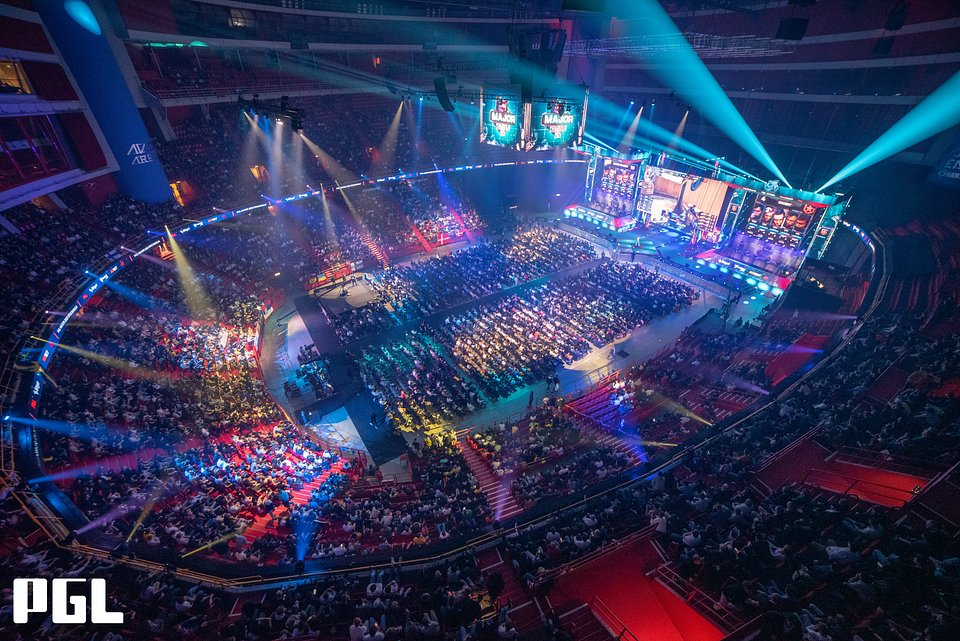
\includegraphics[width=\textwidth]{Figures/major.jpg}
	\caption{The 2021 PGL Major took place in the Avicii Arena in Stockholm, Sweden \cite{pglarticle}}
	\label{fig:major}
\end{figure}

\subsubsection{Gameplay fundamentals}

Counter-Strike is a PC video game played using the mouse, keyboard, and headset. Players assume the role of a soldier in a virtual 3D environment, which can run, walk, and jump by pressing keys on the keyboard. The mouse is typically used for two purposes: to control the direction and movement of the in-game field-of-vision, and for shooting, where cross-hairs at the centre of the player's screen act as the focal point for aiming. For effective communication, players co-ordinate their actions with their team-mates primarily through a headset with a built-in microphone. 

Although a number of versions have been released since its inception, the core game mode played in Counter-Strike, known as \textit{defusal}, has remained relatively unchanged. Two teams of five players each start each round on opposite ends of a virtual arena called a \textit{map}. One team plays the role of the Counter-Terrorists (CT), whose objective is to defend two bomb sites, A and B, from the opposing team, the Terrorists (T). The layout for the popular Counter-Strike map, Mirage, is shown in Figure \ref{fig:mirage}; the red zones highlight the bomb sites and the green zones are the spawn areas for either team. There are seven official maps played in competitive Counter-Strike.

\begin{figure}[h]
	\centering
	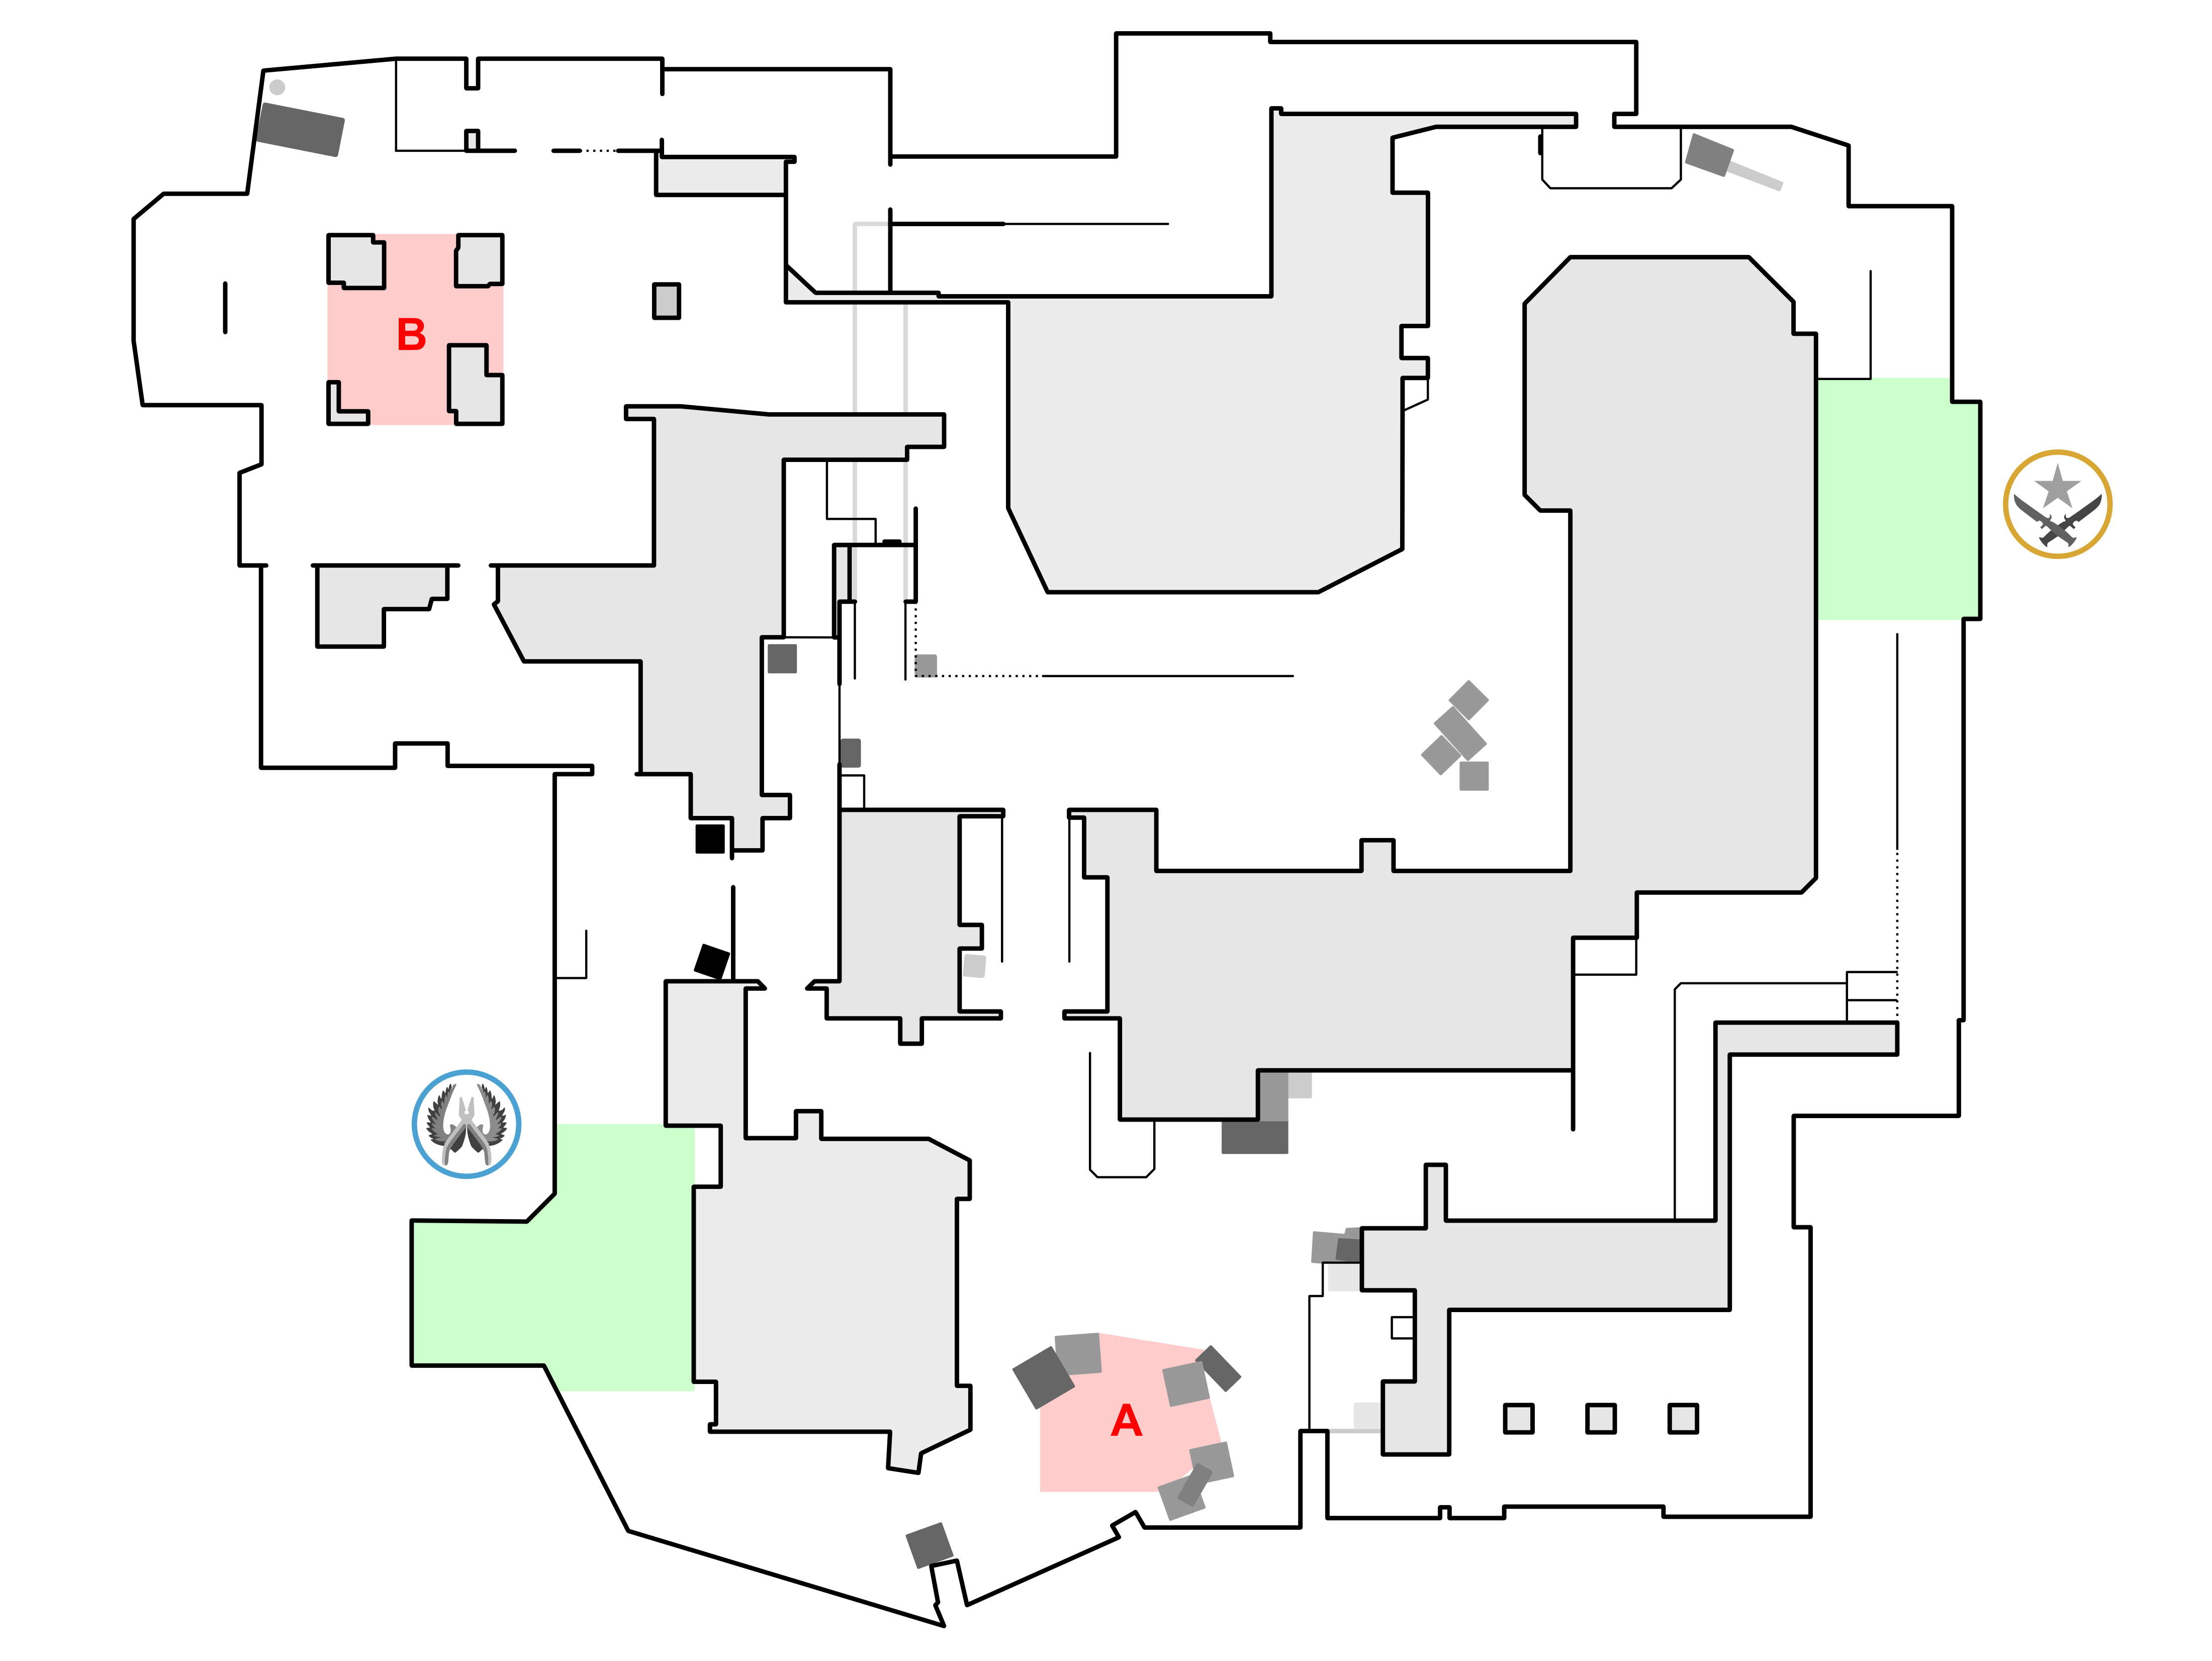
\includegraphics[width=0.9\textwidth]{Figures/mirage.png}
	\caption{Map layout for 'Mirage', showing spawn areas in green and bomb sites in red \cite{mapdiagram}}
	\label{fig:mirage}
\end{figure}

A map is played for best-of-24 rounds, with teams swapping sides after 12 rounds. This means that in order to win, a team must demonstrate superiority over their opponents in both attacking (as Ts) and defending (as CTs). The first team to win 13 round wins the map. In the event of a tie (12-12), the map continues in best-of-6 round \textit{overtime} phases, with sides swapping every 3 rounds, until a winner is decided.

Each round, spanning 1 minute and 55 seconds, is a high-stakes scenario as each player has only one life. Eliminated players have to spectate their living team-mates until the next round. Rounds can be won in four ways: by (1) eliminating the entire enemy team, or, if playing as Terrorists, by (2) detonating a bomb on one of the bomb sites. Once a bomb is planted, the round timer changes to a 40 second countdown until detonation. The Counter-Terrorists can win rounds either by (3) successfully defending both sites for the duration of the round, or by (4) retaking the bomb site and defusing the bomb after it has been planted. Players begin each round with 100 health points (HP). Damage is measured in HP and can be inflicted using a variety of weapons and grenades. There is no way to replenish HP during a round.

\subsubsection{Strategy and team economy in Counter-Strike}

Different strategies (\textit{meta}'s) evolve for attacking and defending the various points on each map, with players learning which positions are optimal to hold with different weapons, how, when, and where to throw their \textit{utility} (smoke, flash-bang, high-explosive, and incendiary grenades), and how to move around the map as the round unfolds. All positions on a given map are named such that players can immediately communicate critical gameplay information to their teammates over the course of a round. Success in Counter-Strike relies on efficient team-work as much as mechanical skill, as player actions need to be co-ordinated in order to optimally assist one's teammates. This can be in terms of positioning (e.g. setting up a cross-fire at a choke point\footnote{A choke point is a small part of the map near each bomb site which, if controlled, gives either team a tactical advantage.}, or moving to help bolster the defence at a bomb site which is being attacked) or in terms of utility usage (e.g. throwing an incendiary grenade at a choke point in order to slow down an attack, or throwing a flash bang to allow a teammate to take control of a position). 

Players are rewarded with in-game money for getting a kill, planting or defusing the bomb, and winning or losing a round. Winning a round is rewarded with far more money than losing a round, however this amount (the \textit{loss bonus}) grows with each consecutive round loss. Money is spent to purchase weapons and equipment at the start of each round. If a player survives the round, they retain whatever equipment they had into the following round. Each team therefore has a monetary balance, known as the team economy, which fluctuates throughout the duration of a map. A stronger economy means you can purchase stronger weapons and more equipment. A weaker economy might relegate your team to just buying a few pistols and practically forfeiting a round in order to save funds for the following round. Sound economic strategy is thus critical to success in Counter-Strike.

At the start of a half, both sides have almost no money and so duel with only pistols. The \textit{pistol round} is quite crucial, as it initiates economic momentum for whichever team wins it. In some exciting cases, teams will defy odds and trade the initial rounds back-and-forth, leaving the economic balance undecided. A game can become extremely tense if both teams have precarious economies near the end, as the outcome is undecided and the stakes get progressively higher. 

The state of each team's economy is a good predictor of their ability to win a given round. This is the total team balance as well as their current loss bonus; teams earn progressively more money with consecutive round losses up to a cap of \$3400 after 5 losses in a row - matching the round-win bonus. A team with the funds to 'full-buy' will almost always win a round against a team that is saving their money in an \textit{eco} round where  they don't purchase anything other than pistols. A \textit{semi-buy} is a middle-ground, used to save enough funds to ensure a \textit{full-buy} the following round, but still giving the team a fighting chance. These distinctions therefore refer to the strength of the weapons and amount of utility grenades that can be purchased in each round.

An example of the economy for two teams over the course of a map is shown in Figure \ref{fig:economy}. The lines corresponds to either team's balance, and a coloured icon represents a round won by the CTs (blue) or the Ts (orange) respectively. The horizontal lines are thresholds that indicate the health of the economy, indicated as eco, semi-buy, and full-buy. Note that the pistol rounds take place in rounds 1 and 13, and teams switch sides in round 13 which results in the round-win icon colour switching.

\begin{figure}[h]
	\centering
	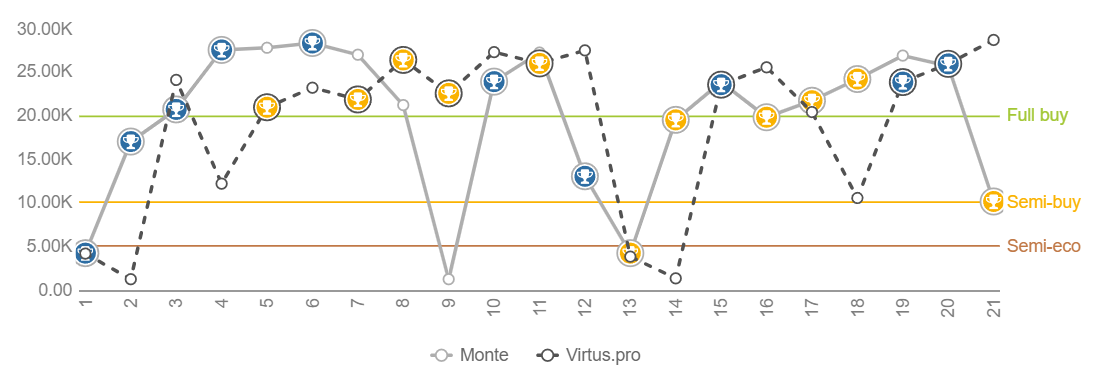
\includegraphics[width=\textwidth]{Figures/economy.png}
	\caption{A graph showing the economies of two teams over the course of a map \cite{vpmatch}}
	\label{fig:economy}
\end{figure}


\subsubsection{Professional Counter-Strike}

The local area network (LAN) is the most competitive environment possible, as all players have the same, virtually instant network latency and there is no possibility for gameplay 'lag'. They play under the same conditions and use identical computer hardware (except for their keyboards and mice). Tournaments played "on LAN" represent the pinnacle of competitive Counter-Strike, with teams flying all over the world to attend these events. Teams qualify for LAN events either through invitation (due to their position in the world ranking), or by placing sufficiently high enough in qualification rounds that are normally played online.

Professional CS matches are played in a best-of-1 (BO1) or best-of-3 (BO3) maps format. The grand final for bigger tournaments are occasionally contested in a best-of-5 (BO5) map series. Match lengths can vary greatly depending on the format and skill-disparity between competitors. A BO1 can be concluded in 20 minutes if one team dominates the other. In extreme cases, a BO5 grand final between two evenly matched giants can become a five-hour affair as tightly-contested maps get traded back-and-forth. The most common format is the BO3, where the match winner is determined over 2 or 3 maps which last roughly 40 minutes each.

Although CS is a methodical and tactical team-based shooter, it is highly dynamic in the short, medium, and long term. During individual rounds, players must make split-second decisions to react to events as they unfold. Over the course of a map of 24 rounds, teams need to learn and adapt to their opponent's habits in order to exploit their weaknesses. Between matches, teams will often adopt and improve strategies from other teams by reviewing their gameplay recordings, or come up with entirely new approaches to counter a certain prevailing strategy.

Teams have coaches whose role is to identify these trends mid-match and suggest appropriate countermeasures. The better-resourced teams employ analysts who review their opponent's games and develop strategies in advance. Competitive CS is mentally demanding, so teams often have sports psychologists to keep the players operating at peak performance \cite{sportspsych}. Throughout the match, coaches must ensure their players maintain composure. As discussed earlier, the longer format matches can become a battle of mental endurance. This has led to some controversy surrounding esports players and the use of stimulants like Adderall \cite{adderall}.

\subsubsection{Data in Counter-Strike}

Every second of CS game generates a wealth of data; in previous versions of the game, the 'tick rate' is the frequency at which each player's game client is synchronized with the server. Professional matches were played exclusively on '128-tick', which means there were 128 snapshots of the game being generated each second, containing every minute detail of the game: each player's precise location on the map, the direction at which they are aiming, and the state they are currently in - moving, jumping, shooting, throwing a grenade, reloading, switching weapons, planting or defusing a bomb, shooting or being shot at. At any given point there can be a number of smoke grenades deployed on a map, a high-explosive grenade being lobbed towards an enemy position, or an incendiary grenade temporarily blocking a choke point. 

With the introduction of CS2's sub-tick system, the granularity of data has been further enhanced, as player movements and interactions can now be recorded in-between ticks using an interpolation system. It should be evident that there is a tremendous amount of data generated in each map played. This gameplay data is stored in a \textit{demo file}, which can be replayed at a later stage or processed for data analysis.

A number of statistics can be generated by processing these demo files. For example, player performance can be measured by the number of kills, deaths, assists, average damage per round (ADR), and weapon accuracy. Free online tools like Leetify rate all players from the data in their match demo-files. They report statistics such as \textit{cross-hair placement precision}, which refers to the degree deviation of the cross-hairs from an enemy who comes into view, \textit{time-to-damage}, which is the number of milliseconds between seeing an enemy and inflicting damage, and \textit{headshot accuracy}, which is the proportion of kills attained by lethal headshots. \textit{Clutch} statistics refer to the percentage of rounds won where a player is last alive on his team versus 1, 2, 3, 4, or 5 opponents. All of these data points help to paint a descriptive picture of a player's contribution to their team's success or defeat. That said, some roles, such as \textit{support} or \textit{in-game leader} (IGL) help their team in ways that are harder to quantify.

Team performance is usually measured by their win-rates on the various maps. Teams have preferred maps, and most also have \textit{perma-bans} which they never play. In a BO3 series, teams will decide which of the 7 maps to play through a veto process; this always follows a ban-ban-pick-pick-ban-ban-decider sequence. There are therefore trends in which maps a team will play and will avoid. A map-veto which favours one team in an otherwise equal match-up can therefore make for a favourable bet. \label{vetoprocess}

All these statistics are prominent features of a professional broadcast; for example, commentators will refer to the weapon accuracies when contrasting the snipers of opposing teams. Dominant teams can go on significant match or map-win streaks, which adds further tension to tight matches. On certain broadcasts, there is a round-win prediction percentage which sways depending on the round economy and number and health of players alive on each side.


\subsection{Machine learning}

\textit{Machine learning} (ML) is an interdisciplinary field, spanning computer science, statistics, and data science. It refers to the development and study of statistical algorithms that can learn from data and generalize to unseen data \cite{mlbook}. It is fitting that the term was coined in 1959 by Arthur Samuel, who, while working at IBM, invented a program to calculate the chances of either side winning in the game of checkers \cite{mlcheckers}. In the last two decades, improvements in computational power has allowed the field to develop from a theoretical concept into a practical technology with widespread commercial use. Today, machine learning methods are employed across a plethora of industries, including health care, manufacturing, education, financial modelling, and more \cite{mltrends}.

ML is considered a subset of artificial intelligence (AI), as many of the algorithms imitate the way that humans learn \cite{mlibmdef}. ML techniques are used for the development of software that perform computer vision, speech recognition, natural language processing, and much more. It is normally far easier to train a system using large amounts of data than it is to explicitly program it to anticipate a desired response for all possible sets of inputs. This makes ML an effective tool for many "big data" applications \cite{mltrends}.

There are three broad categories of machine learning paradigms, which differ primarily on the nature of the feedback available to the learning system. These are (1) supervised learning, (2) unsupervised learning, and (3) reinforcement learning. In \textit{supervised learning}, the system learns from data with known outputs. In other words, the goal is to learn how to map a series of inputs to a series of outputs. It is commonly found in applications like image recognition. In \textit{unsupervised learning}, there are no known output labels and the goal is to learn hidden patterns or structures in the data. An example of this is customer segmentation in marketing. Finally, in \textit{reinforcement learning}, an agent tries to achieve a goal in a dynamic environment known as the problem space. As it navigates the problem space, it is rewarded for good responses and punished for bad ones. The system attempts to optimize the proportion of good responses. This ML paradigm applies to areas such as robotics and game playing.

For this research, the objective is to predict the probability of either team winning given a large dataset of information about two teams. The problem can be expressed as predicting whether Team A will beat Team B, with a binary answer of no, they lose (0), or yes, they win (1). Given that the input data is derived from a large dataset of match records with known outcomes, supervised learning techniques are pertinent. In the subsequent chapter algorithms which have shown promise in sports analytics will be explored.

\section{Research problem}

The techniques used by bookmakers to compile betting odds are not well-represented in the literature. Furthermore, esports betting is a high-growth segment of the market, and professional Counter-Strike matches drive a significant amount of online betting activity. Counter-Strike is a complex esport, with several factors making it difficult to predict. While existing literature has explored machine learning in traditional sports, its application in esports, particularly in Counter-Strike match prediction, remains underexplored. Fortunately, an abundance of data is generated during these matches by virtue of their digital nature, making them an ideal subject for investigation. This study aims to explore whether machine learning techniques can be used to make accurate predictions, and by extension, betting odds estimations, for professional Counter-Strike matches. 

\section{Research objective}

The primary objective of this study is to develop a model that can estimate the odds of either team winning for any given match of professional Counter-Strike. This objective can be broken down into a number of smaller objectives:

\begin{enumerate}
	\item Review the literature on the technology used in the sports betting industry, and on the application of machine learning techniques for sports prediction
	\item Gather a significant dataset of historical data for professional Counter-Strike matches
	\item Identify and generate relevant features from the historical match data
	\item Train a selection of supervised learning models to generate probability estimates and betting odds for either team winning
	\item Measure and compare the performance of each model using classification accuracy and F1-score, and identify the most relevant features for match prediction
	\item Compare the betting odds generated by the models to actual historic betting odds
\end{enumerate}

\section{Scope and limitations}

Although this minor dissertation is concerned with the esports betting industry, it is not feasible to create a model that can predict the outcome for every esport. This is because there are a large variety of esports with different competition rules, gameplay factors, and players. It was therefore decided to focus on one specific esport: Counter-Strike.

In Counter-Strike, there are many betting opportunities beyond just the match winner. As discussed earlier, matches are played in different formats consisting of one or more maps of gameplay. Bettors are often given the opportunity to place bets on which team will win the current map, which team will win the pistol round for a given map, or which team will simply get the first kill of a map. Although map-specific data is used for feature selection, the objective of this research is to quantify probabilities for winning the entire match. The most common match format is Best-of-3 maps, which will be considered the default for this project.

Furthermore, in recent years, live or in-play sports betting has become popular; bettors can make bets while a match is being played, and often cash-out their existing bets for some discounted return. Bookmakers offer dynamic odds which rely on live match analysis. While some research has been done in the field of real-time match prediction, this project will focus purely on predicting the overall match outcome using only historical information, i.e. before the match has begun.

Finally, bookmakers can to some extent monitor market dynamics as they know which bets are being made. They can therefore factor in the market expectations by adjusting the odds offered on different outcomes using the betting information available to them. This data is privy to the bookmakers and will thus not be included in the modelling process.

\section{Ethics approval}

This project was approved by the Commerce Research Ethics Committee with code COM/00541/2023. The approval letter has been included in Appendix \ref{dix:ethics}.

\section{Structure}

This dissertation is comprised of five chapters. The introduction covers the background knowledge relevant to the topic, defines the research problem, and establishes the objectives. Thereafter,  existing research on the esports betting industry and data-driven match prediction is covered in the literature review. 

The third chapter precisely describes the methodology employed to achieve the research objects: how the data is collected, stored, processed, analysed, and used to generate the features. The models selected and the techniques used to train them are all described in this chapter. This chapter is concluded with a description of the script which takes a match input and generates the betting odds. 

The penultimate chapter is a discussion of the results obtained in the modelling process, and how well the objectives were met. Finally, a conclusion summarizes the key findings, limitations, and suggestions for areas of future research.
\chapter{Literature Review}
\label{Literature Review}

This chapter builds upon the topics covered in the background by reviewing relevant academic literature. The development and features of the online sports betting industry are first described, followed by an investigation into how machine learning is used for sports prediction. The specific machine learning techniques used in the literature are researched to better understand how they can be used for Counter-Strike match prediction. Additionally, various rating systems used in sports and esports are identified and discussed. The chapter concludes with a discussion of predictive analysis in esports. 

\section{The evolution of online sports betting}

Technological advances have caused major shifts in gambling practices over the last two decades. The modern sports betting industry utilizes software engineering, data analysis, and real-time processing to satisfy a rapidly growing market of bettors. Bets are overwhelmingly made through the use of a smartphone app or website, where algorithms are used to set and dynamically update betting odds \cite{inplay}. Prior to this revolution, bets would need to be made either in-person or with an operator over the telephone. Bookmakers would employ teams of statisticians, known as odds compilers, whose job was to spectate sports events or horse races, break them down into fundamental inputs, and calculate probabilities from those inputs. Most statistical odds compiling was done by counting the occurrences of a given event. The development of in-play betting caused a shift towards mathematical modelling for odds compilation, as humans could simply not keep up with multiple simultaneous events unfolding: "\textit{Bookmakers needed automation, which meant models}" \cite{oddscompiler}.

Betfair were one of the pioneers in the industry, leveraging technology to offer a superior value proposition to bettors in the form of a peer-to-peer betting exchange. The platform was first developed in 1998 by programmer and professional gambler Andrew Black, whose original idea was to create a betting system which operated like the US stock exchange. By late 2004, Betfair had over 300 000 customers and saw over GBP 50 million revenue per week. A 2005 study on Betfair's competitive advantage cited Moore's Law, Metcalfe's Law of Networks, and the internet as key enablers of its success. \cite{betfair}.

A betting exchange works by offering two types of bets: 'back' and 'lay', where a 'back' is a conventional bet on an outcome to occur, and a 'lay' is betting \textit{against} the outcome happening. Odds are set by the bettors themselves, with a bet only going through if another participant bet on the 'lay'. In this way, no odds compilation is necessary as odds are driven purely by market forces. The exchange operator generates revenue from a much smaller commissions when compared to traditional bookmakers \cite{bettingexchange}.

Another sports betting platform called EmpireBet was the focus of a recent study into sports betting through the lens of software engineering. The authors noted that the biggest drivers of evolution were advances in connectivity, the transition from trained operators to user-friendly interfaces accessible by anyone, the automation of risk management and administration tasks, integration with cloud computing services, and the adoption of third-party libraries for rapid development \cite{empirebet}.

In-play sports betting features, also known as live betting, have been a driver of growth in the industry. This is because bettors can place multiple bets during a single sports event. Many bookmakers now also offer a 'cash-out' feature, which was first introduced to the market by William Hill in 2012 \cite{inplay}. This feature allows bettors to "take profit early" if the outcome you bet on has become more likely, or to gain a fraction of your wager back if it is becoming more unlikely.

As discussed in Section \ref{background-bet}, another driver of growth in the sports betting industry is the development of esports betting \cite{esportsgambling}. Business Research Insights reported the market size as \$ 9.75 billion US in 2021, and projected it to grow to \$ 35.57 billion US by 2023: a CAGR of 13.7\% \cite{esports-betting-market-report}.

\section{Machine learning for sports prediction}

Over the past two decades, there has been a significant growth in the amount of data collected during sports matches, both structured and unstructured. It is no surprise that machine learning algorithms have become increasingly popular for analysis of these increasingly large and complex datasets \cite{mlsports}. 

Statistical prediction of sports outcomes, such as the match winner or final score, is of great interest to spectators, teams, and other industry stakeholders. In 2020, Horvat and Job analysed 38 research papers aimed at this particular application for various team sports, ranging from basketball, football, cricket, baseball, and American football \cite{mlsports}. They found that feature selection was critical for building effective models. Noting that earlier studies relied solely on expert opinions, newer studies could achieve better results using statistical techniques (such as regularization) for feature selection. 

The machine learning models employed by researchers differed depending on the nature of the data and the complexity of the problem. In most of the studies, multiple supervised learning classification models were trained and compared. These included logistic regression, support vector machines, decision trees \& random forests, Naive-Bayes, and gradient boosting. Neural networks (NN) were the most popular technique used for prediction, as they can effectively model non-linear relationships by capturing complex patterns in the data \cite{nnoverview}. 

The models were all trained using either a chronological segmentation of the dataset, or by using k-fold cross validation. The most common way of measuring performance was using classification accuracy. The researchers found significant variance in the performance of the models depending on the sport, the quality of the data, and the feature selection process used. Figure \ref{fig:mlsports} shows the distribution of maximum classification accuracy achieved in the 38 different papers \cite{mlsports}.

\begin{figure}[h]
	\centering
	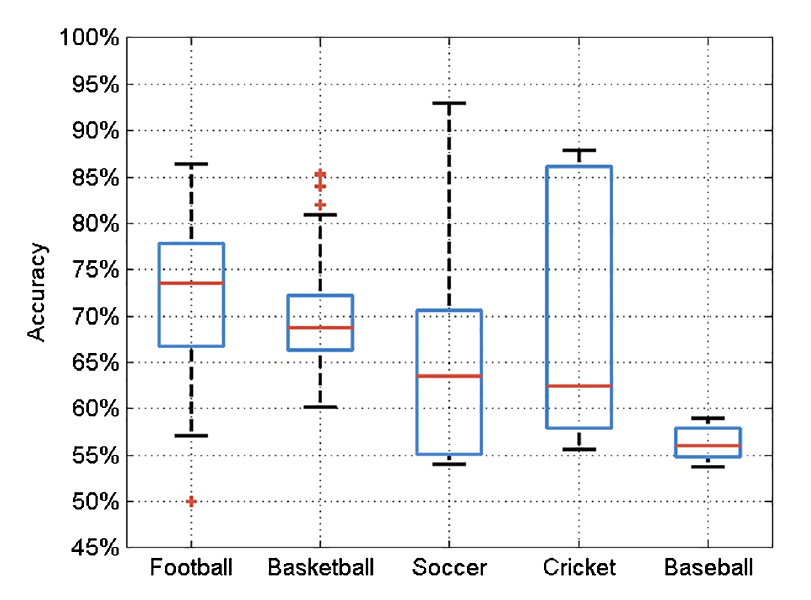
\includegraphics[width=0.8\textwidth]{Figures/mlsports.png}
	\caption{A boxplot of maximum classification accuracies achieved for different sports \cite{mlsports}}
	\label{fig:mlsports}
\end{figure}

Do the same findings apply to esports analysis? Jenny et al. \cite{def-esports} compared esports to traditional sports and argued that, other than the degree of physicality involved, esports display the same characteristics of traditional sports: esports are a voluntary and intrinsically motivated activity, governed by rules, in which opposing players compete. Furthermore, they require skills such as strategic thinking, hand-eye coordination, and rapid decision-making. They concede that the degree of physicality differs significantly, as esports involve fine motor skills as opposed to the high levels of physical exertion typically required in traditional sports. Their research also argued that esports have a global following and are becoming increasingly institutionalized, further cementing their legitimacy. It is therefore reasonable to assume that the techniques described in \cite{mlsports} should, to some extent, be applicable to esports as well. 

\subsection{Machine Learning Algorithms}

In this section the techniques used in the aforementioned papers are investigated. The algorithms include logistic regression, random forest, gradient boosting techniques, support vector machines, and neural networks.

\subsubsection{Logistic regression}

Logistic regression (LR) is a binary classification algorithm: given an input vector $\bm{x_i}$, classify the output label $y_i$ as 0 or 1. The output value is determined by mapping a linear combination of input values onto the logistic function. This produces a probability $p(\bm{x_i})$ of a given input vector $\bm{x_i}$ (set of features) belonging to the default output class, $y_i = 1$. 

\[ p(\bm{x_i}) = \frac{e^{\beta_0 + \beta_1x_{i1} + \beta_2x_{i2} + \ldots}}{1 + e^{\beta_0 + \beta_1x_{i1} + \beta_2x_{i2} + \ldots}}  \]

The optimal set of regression coefficients, ${\beta_0, \beta_1, ..., \beta_n}$, is obtained by maximizing the likelihood function. In LR, the likelihood function is the product of the probabilities $p_i$ of each data point being correctly classified by the model. 

$$\mathcal{L}(\beta_0, \beta_1, ..., \beta_n | y, X) = \prod_{i=1}^{N} p(y_i | \bm{x_i}, \beta_0, \beta_1, ..., \beta_n)^{y_i} \left(1 - p(y_i | \bm{x_i}, \beta_0, \beta_1, ..., \beta_n)\right)^{1 - y_i}$$

where $\mathcal{L}$ is the likelihood function, $y_i$ is the actual label of the $i$-th sample, $\bm{x_i}$ is the feature vector of the $i$-th sample, $\beta_0, \beta_1, ..., \beta_n$ are the regression coefficients, and $p(y_i | \bm{x_i}, \beta_0, \beta_1, ..., \beta_n)$ is the predicted probability of the $i$-th sample belonging to the positive class given the feature vector and coefficients.

Because maximizing the likelihood function is computationally challenging, the negative log-likelihood (also known as cross-entropy loss) function is minimized instead. For logistic regression, the loss function is defined as:

\[ L(y, p) = -\frac{1}{N} \sum_{i=1}^{N} \left[ y_i \log(p_i) + (1 - y_i) \log(1 - p_i) \right] \]

where $L(y, p)$ is the loss function, $N$ is the number of samples, $y_i$ is the actual label, and $p_i$ is the predicted probability that the $i$-th sample belongs to the positive class.

This is an optimization process which is performed iteratively. The logistic regression model therefore fits a logistic curve (also known as a sigmoid) to the data, such that the set of regression coefficients used minimizes the cross-entropy loss function. LR is most appropriate when the class distribution is balanced and a linear relationship exists between the input variables and the output class.

\subsubsection{Decision trees and random forests}

A decision tree resembles a flowchart-structure with three elements: internal nodes which represent different split points on features, branches which represent decision rules, and leaf nodes which represent the outcome. Starting at the top-most node (root), the decision tree is recursively partitioned into progressively smaller sub-trees. In order to make a classification, the tree is traversed using the input features until a leaf node is reached, which indicates the predicted class. There are multiple methods for determining the splitting criterion at each node, such as Information gain (the difference in entropy before and after a split) and Gini impurity. The latter quantifies the 'purity' of a node, with lower values representing more homogenous nodes. In the equation below, $p_i$ is the probability of an observation being classified into the $i^{th}$ class.

\[ Gini\, Impurity = 1 - \sum (p_i)^2 \]

The depth of a decision tree affects its performance and complexity. More complex relationships can be modelled by deeper trees, but these are also more prone to overfitting. 

Overfitting can be mitigated using several techniques. Decision trees can be pruned back according to a cross-validated cost complexity criterion. Their maximum depth can be limited, which prevents them from becoming too complex. The minimum number of samples required to split an internal node can be increased, ensuring that there is enough data to make a decision.

The decision tree in Figure \ref{fig:tree} was generated from data about passengers of the Titanic, with the target class being whether they survived or died. If the passenger were a female, or a male under 10 years old with less than three siblings, the decision tree predicts they would survive. Each leaf node is shown with two values: the probability of survival and the proportion of data points belonging to that node. For example, 61\% of the data points were males aged 10 or more years, of which only 17\% survived.

\begin{figure}[h]
	\centering
	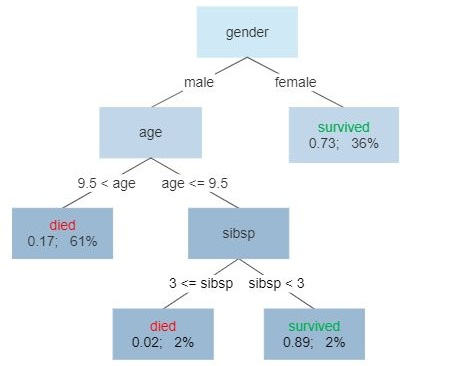
\includegraphics[width=0.7\textwidth]{Figures/decision-tree.jpg}
	\caption{A decision tree for classifying the survival of passengers on the Titanic \cite{fig-tree}}
	\label{fig:tree}
\end{figure}

Random forests is an ensemble model; it combines the outputs of many, simpler decision trees which are each trained on a different random subset of the dataset. This technique is known as bagging and it helps to prevent models from over-fitting the training data. Random forests are typically more robust and have an improved accuracy when compared to a single decision tree. 

\subsubsection{Gradient boosting}

Gradient Boosting is another ensemble technique, however it differs from random forests in that each tree is built sequentially, and learns to 'correct' the errors of the previously trained tree. This process is done by calculating the difference between the predicted and actual values for the initial tree (the residuals), then building a subsequent tree which tries to predict the residuals for the former tree. The model is then updated by adding the weighted tree predictions to the initial predictions. This 'fine-tuning' process is repeated until convergence. 

The learning rate is an important hyperparameter which controls the extent to which each tree's predictions influence the overall model. Lower values often lead to more robust models, however more trees are required for convergence. A fundamental equation in gradient boosting shows how the model is updated using a weighted sum of each learner's predictions. This equation is given by:

\[ F_{new}(x) = F_{old}(x) + \lambda \cdot \sum_{t=1}^{T} \gamma_t \cdot h_t(x) \]

where $F_{new}(x)$ is the updated model prediction, $F_{old}(x)$ is the prediction from the previous iteration, $\lambda$ is the learning rate, $T$ is the total number of trees in the model, $\gamma_t$ is the weight assigned to the t-th tree, and $h_t(x)$ is the prediction of the t-th tree. Each new tree is added to the model iteratively which improves the overall prediction accuracy incrementally.

XGBoost (eXtreme Gradient Boosting) is a popular implementation of gradient boosting which regularly outperforms other models for classification tasks \cite{gradboostingwins}.

\subsubsection{Support vector machines}

Support vector machines are another classification technique whereby a \textit{hyperplane} which optimally separates the data points into their output classes is constructed. The \textit{margin} is the distance between the hyperplane and the nearest data point in each class. A SVM aims to maximize the margin as far as possible. If a linear hyperplane cannot separate the data well enough, the data can transformed into a higher-dimensional space using a \textit{kernel} function.

\clearpage

\subsubsection{Neural networks}

The basic structure of a neural network (NN) consists of large amounts of densely interconnected nodes. In a feed-forward network, data moves in one direction only - forward. It traverses the network from the input layer, through multiple hidden layers of nodes, to an output layer. Figure \ref{fig:feedforward} is an example of this structure. Each node assigns a weight to its incoming connections, and emits an output using an activation function. This function computes an output from each weighted input and a threshold value. During training, the weights and thresholds are adjusted until convergence \cite{nnoverview}. At convergence, these values stabilize and do not change significantly with further training.

\begin{figure}[h]
	\centering
	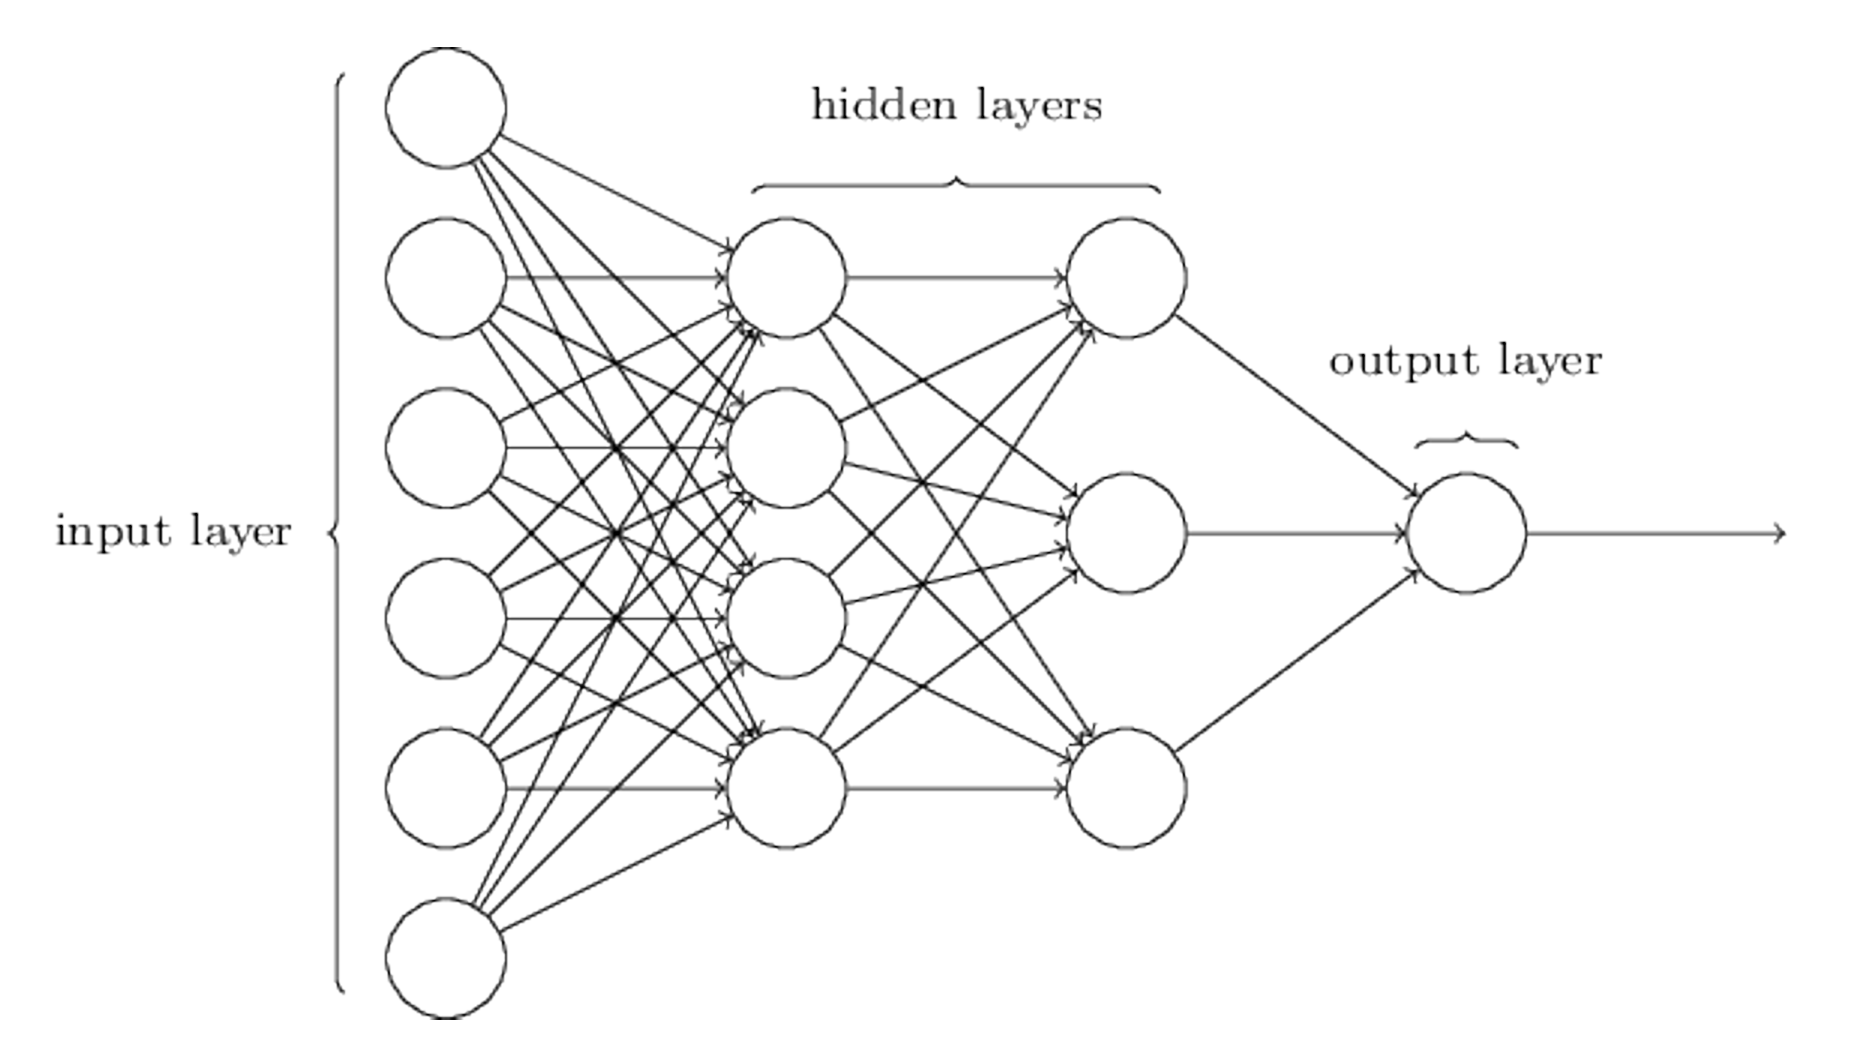
\includegraphics[width=0.8\textwidth]{Figures/feedforward.png}
	\caption{A simple feed-forward neural network \cite{nn_fig}}
	\label{fig:feedforward}
\end{figure}

They key parameters which affect the network's capacity to model complex relationships in the data are the depth of the network (the number of hidden layers) and the width (the number of nodes in each hidden layer). The activation function used must be selected beforehand. A common activation function is the Rectified Linear Unit (ReLU), defined as:

\[ f(x) = \max(0, x) \]

where \( f(x) \) is the activation function applied to the input \( x \) of a neuron.

There are multiple types of neural networks with different applications. Feed-forward neural networks, such as multilayer perceptrons (MLPs), work as described above. MLPs consist of at least three layers of nodes and can be used for both classification and regression tasks. Recurrent neural networks involve back-propagation, where outputs are fed back into the model. Convolutional NNs consist of one or more NNs in 'convolutional layers', which are isolated smaller regions of the feature space. CNNs have been shown to be particularly effective for image recognition and natural language processing applications \cite{cnn-paper}. 

\clearpage

\subsection{Rating systems}

Ratings and ranks are a representation of the relative performance of a given player or team. Although the methods differ, ratings are determined from past performances. There is an implicit expectation that higher-rated teams are expected to beat lower-rated teams more often than not. A good rating system is one which represents the true skill level as accurately as possible.

\subsubsection{Elo}
\label{elo}

The Elo rating system was developed by Hungarian-American physics professor Arpad Elo \cite{elo}. Its original purpose was to rank the strength of different chess players, however it can be applied to any zero-sum game. The Elo system has been used to rate teams and players in many other sports, including football, baseball, and esports. The central idea is that the difference between two players' Elo ratings serves as a predictor of the match outcome. Each player's Elo rating is a single value, $R$. After each game, the winner gains points and the loser loses points. The magnitude of the loss and gain is different for each player, depending on their original Elo ratings. A mathematical description of the Elo rating system follows. 

Let players A and B have initial ratings $R_A = 900$ and $R_B = 1000$. The expected score for player A and B is given by the logistic function with base 10:

\[ E_A = \frac{1}{1 + 10^{(R_B - R_A) / 400}} = 0.360 \]
\[ E_B = \frac{1}{1 + 10^{(R_A - R_B) / 400}} = 0.640 \]

As shown above, the expected outcomes are complements of each other, adding up to $1$. After the match is played, the player ratings are then updated:

\[ R_A^{'} = R_A + K \cdot (S_A - E_A) \]

where $S_A$ is the actual score for player A and $K$ is the maximum possible adjustment per game. Adjusting the $K$-factor will adjust the sensitivity of the system to change. Assuming that player A won the game, $S_A = 1$, and $K = 50$,

\[ R_A^{'} = 800 + 50 \cdot (1 - 0.360) \approx 932 \]
\[ R_B^{'} = 1000 + 50 \cdot (0 - 0.640) \approx 968 \]

Player A's Elo rating has increased, and Player B's has decreased. If the players were to play another game, the expected outcome has now changed to reflect their new ratings:

\[ E_A^{'} = 0.448 \]
\[ E_B^{'} = 0.552 \]

In this way, all players can be rated on the same scale and the probability of winning is easily calculated. In the graph in Figure \ref{fig:elo}, the expected score can be interpreted as the probability of the first player winning. For example, as the difference in Elo rating approaches 800, the probability of the player with the higher Elo rating winning approaches 100\%.

\begin{figure}[h]
	\centering
	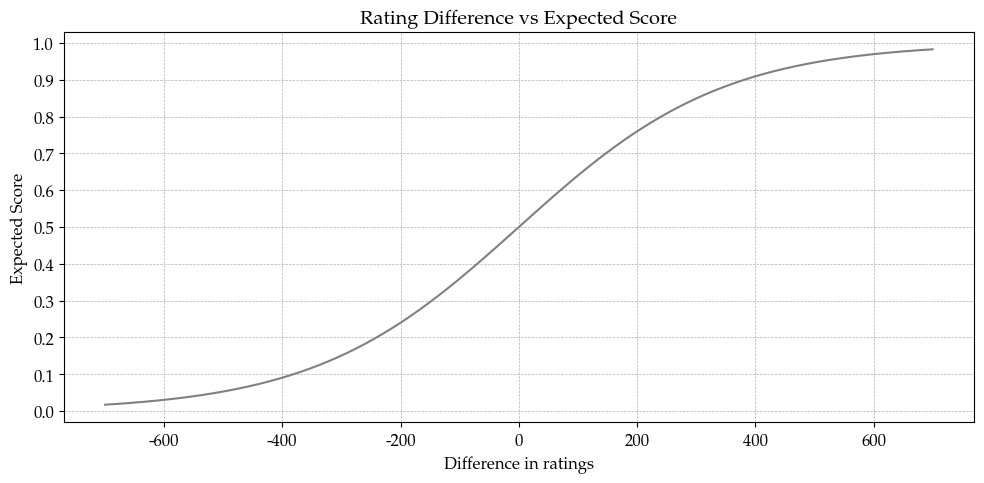
\includegraphics[width=\textwidth]{Figures/elo.png}
	\caption{Difference in player Elo ratings vs expected score}
	\label{fig:elo}
\end{figure}

\subsubsection{Glicko}

In practice, the $K$-factor used in the Elo system is not always held constant. For example, when trying to rank new players, it is sensible to allow their ratings to change rapidly, and decrease $K$ over time, as more games are played and more becomes known about their skill level. The 'Glicko' system, created in 1995 by Mark Glickman \cite{glicko}, introduces the concept of a \textit{Ratings Deviation} (RD), or standard deviation, to account for the uncertainty of a player's rating. A low RD indicates a higher level of certainty about the player's rating, whereas a high RD is typical for players who compete infrequently or only have a few games played.

A central idea to the Glicko system is the \textit{rating period}. Ratings and RD are determined for each player at the start of a new rating period:

\[
RD = \min \left\{ \sqrt{RD_0^2 + c^2t}, 350 \right\}
\]

The expected score for player A against player B is then given by:
\[
E_A = \frac{1}{1 + 10^{g(RD_B) \cdot (R_B - R_A) / 400}}
\]
where \( g(RD) \) is a function that scales the influence of the rating deviation.

The updated rating and rating deviation for player A after a series of games is calculated as:
\[
R_A' = R_A + \frac{q}{(1/RD_A^2) + (1/d^2)} \sum_{i=1}^{n} g(RD_i)(S_i - E_i)
\]
\[
RD_A' = \sqrt{\left(\frac{1}{RD_A^2} + \frac{1}{d^2}\right)^{-1}}
\]
where \( q \) is a constant, \( d^2 \) is a term derived from the expected scores and outcomes of the games played, and \( n \) is the number of games played in the rating period.

In contrast to the Elo system where both players' ratings change by the same magnitude, in the Glicko system this amount is governed by their opponent's RD.

\subsubsection{TrueSkill\texttrademark}

TrueSkill\texttrademark{} is a skill rating system designed by Microsoft Research and published in January 2007 \cite{trueskill}. TrueSkill was designed specifically for multiplayer online games, with the intention of matching players together with similar skill levels such that the games were more "enjoyable, fair, and exciting". Each player's skill level is modelled as a Gaussian distribution, $\mathcal{N}(\mu, \sigma^2)$, where $\sigma^2$ is the variance of the distribution, and a smaller value reflects higher confidence in the player's skill level $\mu$.

New players start with a default skill distribution. After each match, Bayesian inference is used to update and predict players' skill levels, using pairwise comparisons between each player in each team. These comparisons are evaluated using the cumulative distribution function of the difference of two players' TrueSkill ratings, which is also a Gaussian. The expected probability of player A beating player B can therefore be calculated as:
\[P(A \text{ beats } B) = \Phi\left(\frac{\mu_A - \mu_B}{\sqrt{\sigma_A^2 + \sigma_B^2}}\right)\]
where ($\Phi$) is the cumulative density function of the standard normal distribution, ($\mu_A$) and ($\mu_B$) are the skill estimates of players A and B respectively, and ($\sigma_A$) and ($\sigma_B$) are their corresponding uncertainties.

Over time and with more games played, the standard deviation $\sigma$ of a player's skill distribution decreases, reflecting increased confidence in their skill level estimation.

TrueSkill\texttrademark{} expands upon the foundations of Elo and Glicko, with key advances being the ability to rate each individual in a team of players, and allowing for matches of more than two players or teams to to be modelled. For team games, TrueSkill treats the team's skill as the sum of the skills of its members. In their research paper, Herbrich et al.  \cite{trueskill} demonstrated that TrueSkill worked well in their experiments with hundreds of thousands of Xbox Live players.

\section{Predictive analysis in esports}

Esports have the unique characteristic of being natively digital. This means that recording data from a given match is much cheaper and easier than traditional sports, and even amateur games can be recorded in fine detail. In the age of \textit{big data}, esports are therefore well-positioned for data analysis. 

This is reflected by the significant number of papers that have been written on the topic of prediction in different esports, with a particular emphasis on real-time match analysis. Hodge et al. \cite{livematchprediction} performed a comprehensive case study on live win prediction in Dota~2, and concluded that win prediction is difficult, where no single technique excels. They suggested combining techniques into ensembles to achieve better performance. These events were combined with pre-game information to construct the feature set. The ML algorithms used were logistic regression, random forests, and LightGBM, a performant gradient-boosting algorithm. They found that LightGBM outperformed both logistic regression and random forest. Dota~2 matches last 40 minutes on average but can be as short as 10 minutes. Noting a shortage of professional matches to use for analysis, their approach was to use an input data set of 5744 game replays from highly rated, but not necessarily professional players. The dataset was chronologically split, with two-thirds for training and the remainder for testing. They further tested their models on a significantly smaller set of 186 tournament matches. Despite a poor pre-match prediction accuracy of 55.8\%, they found that when using features known 20 minutes into the game (the average half-way point of a match) they could predict the winner of professional games with 74.59\% accuracy.

A similar study was conducted by Yang et al. \cite{yang2016realtime}, with an expanded dataset of 78263 Dota~2 matches. By considering player history, they could improve the pre-match feature set. This allowed the authors to achieve a 71.49\% accuracy using logistic regression and 70.46\% using neural networks. With live prediction, they found that a key factor affecting performance was the time of the match, with real-time features becoming increasingly informative as the match progresses. At the 40th minute of the match, their model achieved 93.73\% prediction accuracy.

A number of studies have been done on different aspects of Counter-Strike gameplay. Bednárek et al. \cite{demofileprocessing} described how to accurately parse data from demo files, which often contained inconsistencies or errors. They also described how player identities could be linked from the demo files to their online player profiles. The extracted demo-file data is ripe for live feature generation; Marshall et al. \cite{livedeaths} used convolutional and recurrent neural networks to predict the probability of a player dying within the next 5 seconds. The input features were recorded from 542 matches, with 5 second windows of information containing features related to damage events. They found long short-term memory, a form of recurrent neural network, yielded the best performance.

Xenopolous et al. \cite{wpacs} created a framework, known as 'Win Probability Added', for valuing individual player contributions to their team's round-win percentage. They extracted over 70 million data points from 4682 demo files. Their research employed machine learning models such as logistic regression and gradient boosting (CatBoost and XGBoost) to generate the win probabilities. Another study \cite{spendingerror} focused on modelling 'Optimal Economic Decisions' for a given round in CS. This study employed XGBoost and neural networks on a dataset derived from 6538 demo files. They found a correlation between spending errors and lower round win-rates.

Some research has been done in pre-match CS win prediction. Švec \cite{svec} used online match data to train machine learning models to predict match winners. They achieved 60\% classification accuracy using graph convolutional networks, which was "disappointing" when compared to the performance attained with a comparatively simple Elo-based baseline prediction. Another study \cite{mapvetoml} aimed to create a decision support system to estimate the win probability for a given map. The researchers trained a linear regression and random forests model with player data from FACEIT, a popular third-party match-making service. They managed to attain an overall match prediction accuracy of 57.42\%. A similar study \cite{faceitclusters} used k-means to cluster players together using data from their FACEIT matches. Once clustered, the player data was used to train a feed-forward neural network to determine their win probability. An accuracy of 65.11\% was obtained, which exceeded their benchmark prediction made from win-rates alone.

\section{Summary}

It is evident that sports prediction using machine learning techniques is a popular field of research. The key factors affecting performance are the quality of data used, the features that can be derived, the choice of ML algorithms, and the sport in question \cite{mlsports}. Unpredictability is an inherent characteristic of sports, and esports are no different.

The studies surrounding Counter-Strike match prediction are noteworthy, however more work can be done to expand upon the results obtained: the quality and quantity of data, as well as the features derived therefrom, can be improved. Furthermore, studies typically measure the performance with respect to statistical metrics, such as classification accuracy, F1-score, and AUC. By expanding the scope of the study to generate betting odds, a comparison with real-world betting odds can be made, which may produce novel and valuable insights into the ever-expanding industry of online sports betting. 
\chapter{Methodology}
\label{Methodology}

All programming for this dissertation was written in Python \cite{python} and the source code is accessible on \href{https://github.com/zakdux/counter-strike}{GitHub}.

\section{Data Collection}

\href{https://www.hltv.org/}{HLTV} is a household name in the Counter-Strike scene. Since its inception in 2002, it has evolved from a repository of CS 1.6 match recordings to a hub for all things Counter-Strike: fixtures, news articles, player interviews, and much more complement an enormous public database of match statistics. 

Every professional and most semi-pro teams are tracked on HLTV; an extensive array of statistics for every match played at every tournament is reported. Furthermore, game play recordings, known as demo files, are hosted for the majority of high-level matches. These demo files can be downloaded and replayed to recreate each second of a given match.

\href{https://liquipedia.net/counterstrike/}{Liquipedia} is a viable alternative to HLTV; it is a collaborative online encyclopedia (a wiki) with records dating back to the very first CS tournament. Ultimately, HLTV was selected for its easy-to-navigate interface and increased depth of statistical data. Unlike Liquipedia, however, HLTV does not provide an API for retrieving the match data at scale. Thus a web-scraping solution is required. A web-scraper is a program which can automatically request, download, and parse information from web pages.

\subsection{Requirements}

The development requirements for data collection were therefore to:

\begin{enumerate}
\item{Design a database to store desired match, map, and player data}
\item{Automatically download relevant match pages from HLTV}
\item{Parse information from the pages and store it in a database}
\item{Synchronize the database with the latest HLTV data}
\end{enumerate}

The following Python packages were identified as suitable for meeting these requirements:
\begin{itemize}
\item{\textbf{SQLAlchemy}, for object-relational mapping to a \textbf{SQLite} database}
\item{\textbf{ZenRows}, for efficiently downloading pages from HLTV}
\item{\textbf{BeautifulSoup}, for reading and extracting data from downloaded pages}
\end{itemize} 


\subsection{Database design}

%The database should be designed to comprehensively store historic match information. This means that it can include details about each match, which maps were played, which players played on each team, and how well they performed. The table schemas were designed by observing which information on the HLTV pages are relevant.

\subsubsection{Matches}

Every professional game of Counter-Strike is represented on HLTV by means of a \textbf{match} page. These list a wealth of information, such as the teams playing, the maps played, and the map veto sequence. There are also links to watch recordings of the match or download the demo file. An example of a match page is shown in Figure \ref{fig:match_cropped}. The schema shown in Table \ref{tab:match} was determined after considering which data on the match page is relevant to the project.

\begin{figure}[h]
	\centering
	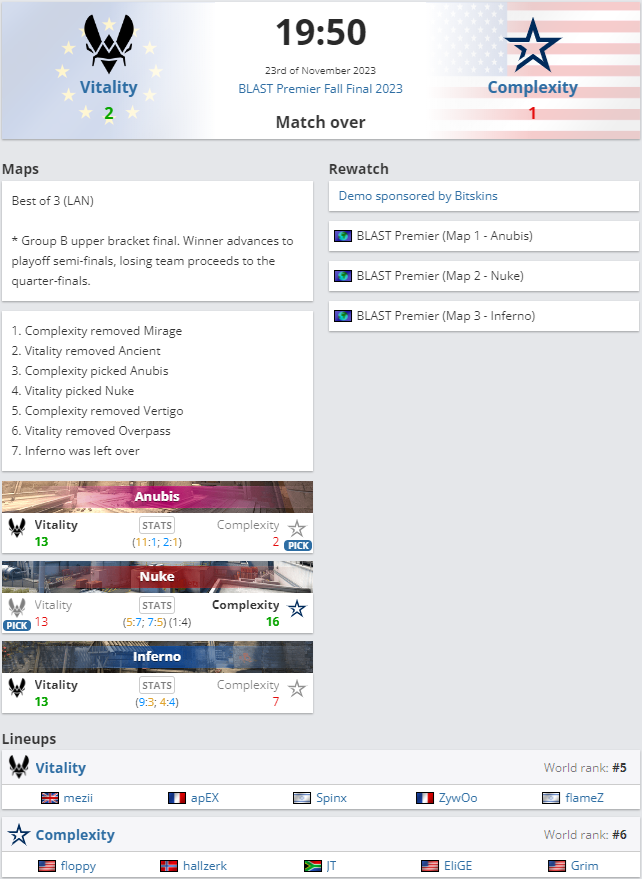
\includegraphics[width=0.9\textwidth]{Figures/hltv/match-cropped-3.png}
	\caption{An HLTV \href{https://www.hltv.org/matches/2368036/vitality-vs-complexity-blast-premier-fall-final-2023}{match page} for Vitality versus Complexity (cropped)}
	\label{fig:match_cropped}
\end{figure}

\begin{table}[h!]
	\centering
	\caption{Simplified schema for the \texttt{match} table}
	\renewcommand{\arraystretch}{1.2} % Adjust vertical spacing
	\begin{tabular}{|>{\ttfamily}l|>{\ttfamily}c|l|}
		\hline
		\multicolumn{1}{|c|}{\textnormal{\textbf{Field}}} & \multicolumn{1}{c|}{\textnormal{\textbf{Type}}} & \multicolumn{1}{c|}{\textbf{Description}} \\
		\hline
		id & INTEGER & Match ID, the primary key\\
		\hline
		datetime & DATETIME & Date and time at start of match\\
		\hline
		team1\_id & INTEGER & Identifier for the first team \\
		\hline
		team2\_id & INTEGER & Identifier for the second team \\
		\hline
		team1\_score & INTEGER & Number of maps\footnotemark[1] won by first team \\
		\hline
		team2\_score & INTEGER & Number of maps\footnotemark[1] won by second team \\
		\hline
		event\_id & INTEGER & Identifier for the event\\
		\hline
		event & STRING & Name of the event\\
		\hline
		lan & BOOLEAN & Indicates if the match was played on a LAN or online\\
		\hline
		best\_of & INTEGER & The match format (1/3/5)\\
		\hline
		box\_str & STRING & Extra details reported on match page\\
		\hline
		veto & STRING & The order of the map veto process\\
		\hline
		cs2 & BOOLEAN & Indicates if match was played in CS2 or CS:GO \\
		\hline
	\end{tabular}
	\label{tab:match}
\end{table}

\newpage

The five players that make up each team are reported at the bottom of every match page in the 'Lineup' section. This information is useful to record as rosters change over time and players are sometimes substituted. It was thus decided to record the two line-ups for every match in a separate table. This schema is shown in Table \ref{tab:lineup}.

\begin{table}[h!]
	\centering
	\caption{Simplified schema for the \texttt{lineup} table}
	\renewcommand{\arraystretch}{1.2} % Adjust vertical spacing
	\begin{tabular}{|>{\ttfamily}l|>{\ttfamily}c|l|}
		\hline
		\multicolumn{1}{|c|}{\textnormal{\textbf{Field}}} & \multicolumn{1}{c|}{\textnormal{\textbf{Type}}} & \multicolumn{1}{c|}{\textbf{Description}} \\
		\hline
		id & INTEGER & Lineup ID, the primary key \\
		\hline
		team\_id & INTEGER & Identifier for the team \\
		\hline
		rank & INTEGER & HLTV team rank at that time \\
		\hline
		match\_id & INTEGER & Identifier for the associated match \\
		\hline
		player1\_id & INTEGER & Identifier for the first player \\
		\hline
		player2\_id & INTEGER & Identifier for the second player \\
		\hline
		player3\_id & INTEGER & Identifier for the third player \\
		\hline
		player4\_id & INTEGER & Identifier for the fourth player \\
		\hline
		player5\_id & INTEGER & Identifier for the fifth player \\
		\hline
	\end{tabular}
	\label{tab:lineup}
\end{table}

\footnotetext[1]{In a BO1, the score is the number of rounds won}
\clearpage

\subsubsection{Maps}

\label{maps}

Clicking on any of the individual map results listed on the match page will load the \textbf{map} page. These pages report more granular data for  each map that was played in the match. A BO3 match, for example, consists of either two or three maps, all of which will have their own map page with detailed statistics. An example of a map page is shown in Figure \ref{fig:map_cropped}, which was retrieved by clicking on the 'STATS' button on the corresponding tile on the match page. The schema shown in Table \ref{tab:map} was determined after considering which data on the match page is relevant to the project.

\begin{figure}[h!]
	\centering
	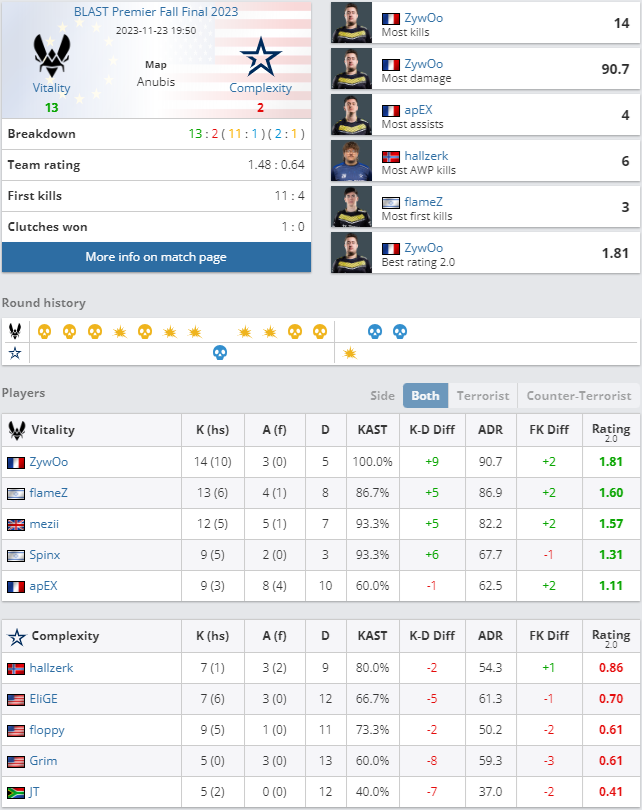
\includegraphics[width=0.9\textwidth]{Figures/hltv/map-cropped-2.png}
	\caption{A \href{https://www.hltv.org/stats/matches/mapstatsid/167162/complexity-vs-vitality}{map page} for the first map played, Anubis, in the match between Vitality and Complexity (cropped)}
	\label{fig:map_cropped}
\end{figure}

\clearpage

\begin{table}[h]
	\centering
	\caption{Simplified schema for the \texttt{map} table}
	\renewcommand{\arraystretch}{1.2} % Adjust vertical spacing
	\begin{tabular}{|>{\ttfamily}l|>{\ttfamily}c|l|}
		\hline
		\multicolumn{1}{|c|}{\textnormal{\textbf{Field}}} & \multicolumn{1}{c|}{\textnormal{\textbf{Type}}} & \multicolumn{1}{c|}{\textbf{Description}} \\
		\hline
		id & INTEGER & Map ID, the primary key \\
		\hline
		match\_id & INTEGER & Identifier for the match \\
		\hline
		t1\_id & INTEGER & Identifier for Team 1 \\
		\hline
		t2\_id & INTEGER & Identifier for Team 2 \\
		\hline
		map\_name & STRING & Name of the map \\
		\hline
		t1\_score & INTEGER & Rounds won by team 1\\
		\hline
		t2\_score & INTEGER & Rounds won by team 2\\
		\hline
		t1\_rating & FLOAT & Team 1 HLTV rating \\
		\hline
		t2\_rating & FLOAT & Team 2 HLTV rating \\
		\hline
		t1\_first\_kills & INTEGER & Team 1 first kills \\
		\hline
		t2\_first\_kills & INTEGER & Team 2 first kills \\
		\hline
		t1\_clutches & INTEGER & Team 1 clutches\footnotemark[2] \\
		\hline
		t2\_clutches & INTEGER & Team 2 clutches\footnotemark[2] \\
		\hline
		t1\_round\_history & STRING & Team 1 round outcomes \\
		\hline
		t2\_round\_history & STRING & Team 2 round outcomes \\
		\hline
	\end{tabular}
	\label{tab:map}
\end{table}


\footnotetext[2]{A clutch is when all of a player's teammates are eliminated and they still win the round}

Each player's \textbf{performance} on a given map is reported on the table on the map page. Their performance is measured by a number of statistics, such as their kill-death ratio (KDR), average damage per round (ADR), and flashbang assists. These are described in table \ref{tab:playerstats}.

\begin{table}[h!]
	\centering
	\caption{Simplified schema for the \texttt{playerstats} table}
	\renewcommand{\arraystretch}{1.2} % Adjust vertical spacing
	\begin{tabular}{|>{\ttfamily}l|>{\ttfamily}c|l|}
		\hline
		\multicolumn{1}{|c|}{\textnormal{\textbf{Field}}} & \multicolumn{1}{c|}{\textnormal{\textbf{Type}}} & \multicolumn{1}{c|}{\textbf{Description}} \\
		\hline
		player\_id & INTEGER & Player ID, part of the composite primary key \\
		\hline
		map\_id & INTEGER & Map ID, part of the composite primary key \\
		\hline
		kills & INTEGER & Number of kills by the player \\
		\hline
		hs & INTEGER & Number of headshot kills \\
		\hline
		assists & INTEGER & Number of assists by the player \\
		\hline
		flashes & INTEGER & Number of times a thrown flashbang led to a kill \\
		\hline
		deaths & INTEGER & Number of player deaths \\
		\hline
		kast & FLOAT & Kill/Assist/Survival/Traded (KAST) percentage \\
		\hline
		adr & FLOAT & Average damage per round in hit points \\
		\hline
		first\_kd & INTEGER & Number of times the player got the opening kill\\
		\hline
		rating & FLOAT & HLTV rating \\
		\hline
	\end{tabular}
	\label{tab:playerstats}
\end{table}

\newpage

\subsection{Downloading \& processing}

In order to populate the tables listed in the previous section, the web pages first needed to be downloaded and processed. By separating the scraping process into two discrete steps, downloading and processing, subsequent modifications could be made to the database and processing without the need to request any page data from HLTV a second time. 

The ZenRows package was used to great effect to download the data from HLTV. Many modern websites, including HLTV, make use of Cloudflare and other services to protect against cyberattacks and other malicious traffic. This results in inconsistent responses when issuing requests programmatically. By issuing the requests via the ZenRows API, the rate of successful responses was over 99\%. 

Due to the sheer magnitude of pages of data, concurrency was implemented to vastly improve the rate at which pages could be downloaded and processed. A function was written which initiates ten ZenRows API client instances, loops through the list of URLs, requests each one, and downloads the HTML data in each response. 

The next problem to solve was how to obtain the list of addresses for all the map- and match-pages.

\subsubsection{Finding the map links}

HLTV conveniently has a \href{https://www.hltv.org/stats/matches}{results page} that lists every single map in their database. An example of such a page is shown in Figure \ref{fig:map_urls}. The list can be filtered by event type (Majors, Big events, LAN, or online), date, ranking (where at least one of the teams playing must be ranked in the Top $x$ teams), and Map (Inferno, Mirage, etc.). By navigating through this list, all the desired links to the map pages could be retrieved. This page will henceforth be referred to as the \textit{map-link} page.

\begin{figure}[h]
	\centering
	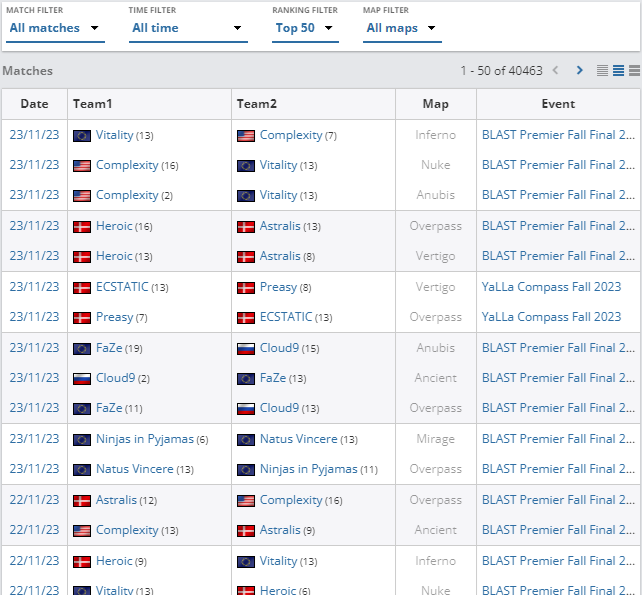
\includegraphics[width=0.9\textwidth]{Figures/hltv/map-urls-cropped-2.png}
	\caption{A map-link \href{https://www.hltv.org/stats/matches?startDate=all&rankingFilter=Top50}{page}, where each row is linked to a different map page}
	\label{fig:map_urls}
\end{figure}

Two noteworthy decisions were made here: to only record data from the last five years (from 2019 to the present), and to only consider matches where at least one of the teams was ranked in the Top 50 teams as reported by HLTV's weekly rankings. This was done to narrow the scope to relatively recent matches played by professional teams.

Each map-link page reports a maximum of 50 map records, which means that the scraper needs to be able to navigate through multiple pages, depending on the amount of rows, to retrieve all the URLs. This was done by downloading the first page, then processing it to find the pagination range. This range was then used to form the list of remaining pages to download.

Once all the map-link pages had been downloaded, the list of URLs to the map pages themselves needed to be extracted. Each file was sequentially processed to isolate the map ID and URL for each map played. Further details could be collected later when the map pages themselves were scraped. This information was stored in its own table, \texttt{map\_url}, along with two flags indicating if the respective map page had been downloaded and whether the map statistics had been processed and stored in the database.

\begin{table}[h]
	\centering
	\caption{Schema for the \texttt{map\_url} table}
	\renewcommand{\arraystretch}{1.2} % Adjust vertical spacing
	\begin{tabular}{|>{\ttfamily}l|>{\ttfamily}c|l|}
		\hline
		\multicolumn{1}{|c|}{\textnormal{\textbf{Field}}} & \multicolumn{1}{c|}{\textnormal{\textbf{Type}}} & \multicolumn{1}{c|}{\textbf{Description}} \\
		\hline
		id & INTEGER & Map ID, the primary key \\
		\hline
		url & STRING & The unique string in the map page URL \\
		\hline
		downloaded & BOOLEAN & Flag indicating if the page has been downloaded \\
		\hline
		processed & BOOLEAN & Flag indicating if the page has been processed \\
		\hline
	\end{tabular}
	\label{tab:map-link}
\end{table}


\newpage
\subsubsection{Downloading the maps and matches}
Once the list of map URLs was recorded, the individual map pages could be downloaded. An example of a map page is shown in Figure \ref{fig:map_cropped}. The majority of the metrics displayed on these pages were recorded in the database, with each map creating one record in the \texttt{map} table and ten records in the \texttt{playerstats} table. These schemas are described in Tables \ref{tab:map} and \ref{tab:playerstats}.

A match can consist of multiple maps. Each map page is therefore related to a corresponding match page. These pages can be accessed using the dark-blue button labelled "More info on match page" on the map page, as seen in Figure \ref{fig:map_cropped}. An example of a match page is shown in Figure \ref{fig:match_cropped}. 

The links to the match pages were recorded in their own table in the database, \texttt{match-links}, in the exact same way as the map URLs were before. The match page contains valuable information such as the match format and veto process. These pages were downloaded and processed to create records in the \texttt{match} and \texttt{lineup} tables.

To summarize, there are two types of pages that display all data relevant to each match: a match page (Figure \ref{fig:match_cropped}) and one or more map pages (Figure \ref{fig:map_cropped}). In order to get to these pages, a list of map URLs first needed to be recorded by navigating through a series of map-links pages (Figure \ref{fig:map_urls}). Each time the scraping program is instructed to fetch new data, it starts by downloading the map-links page(s), then goes to each of the listed map pages, and finally, it downloads the corresponding match pages.

\subsubsection{Processing and synchronization}

Downloading a large number of pages can take a significant amount of time. This was mitigated in two ways, (1) by the use of tracking tables which prevent downloading the same page twice, and (2) by implementing concurrent ZenRows clients. 

Processing thousands of pages of match and map data is an equally pedestrian process. To speed up this step, the processing functions are executed concurrently using multiple CPU threads. A wrapper function was implemented which takes a list of downloaded map or match pages, and initialises a thread pool using the \texttt{asyncio} package. Each thread sequentially reads data from the files, parses the data from the HTML, and returns a dictionary object which is appended to a list. Once all tasks have been completed, these lists of maps or matches are inserted into the corresponding table in the database \textit{en masse}.

Finally, in order to keep the database up-to-date with the latest matches, a synchronization feature was developed. This function performs the full process described above, but starts by filtering the map-links page by the appropriate date range, starting with the last recorded date in the database. The URLs for the new maps can then be retrieved, and all the new pages are then downloaded and processed.

\clearpage


\section{Feature Engineering}

\newcommand{\mapsTotal}{24372}
\newcommand{\matchesTotal}{11271}
\newcommand{\matchesBoOne}{2234}
\newcommand{\matchesBoThree}{8848}
\newcommand{\matchesBoFive}{142}
\newcommand{\datasetStartDate}{2019}
\newcommand{\datasetEndDate}{2023}

\newcommand{\matchesCSGO}{10843}
\newcommand{\matchesCSTwo}{428}
\newcommand{\matchesLAN}{2225}
\newcommand{\matchesOnline}{9046}


The dataset spans every official match played by a Top-50 ranked team between \datasetStartDate{} and \datasetEndDate{}. This range includes a total of \mapsTotal{} maps across \matchesTotal{} matches.

In order to be used for machine learning, this abundance of information needs to first be processed and converted into a dataset of features. The relationship between the input features and the output label is then modelled by each ML algorithm. Each feature is therefore defined from the perspective of one team against an opponent, where the target variable $y$ is a boolean class indicating whether they won the match or not.

The majority of the features are generated from historical match records. Particular care was taken to ensure that no \textit{data leakage} occurred. Data leakage is when the training data contains information about the target variable \cite{leakage}. An example of leakage would be if a win-rate is calculated by including the match being predicted. In other words, only matches played prior to the match in question were included in the calculations for the historical features.

\subsection{Ranks and ratings}

The purpose of any given ranking system is to order the constituents by how good they are. It follows that a higher-ranked or rated team is expected to beat a lower-ranked team. Ratings therefore serve as a proxy for expected performance. That said, there are many ways to rate and rank teams.

\subsubsection{HLTV world ranking}

HLTV maintains a world ranking which is updated weekly. Each team is ranked using a points system; a team will gain points depending on their recent form and their placement in LAN tournaments. There is an element of points-decay, where older achievements become progressively more irrelevant. In the event of roster changes, teams are required to retain at least 3 'core' players, otherwise their points will be lost \cite{hltv-ranking}.

A team's world ranking is a good indicator of their skill level; one would expect the No. 1 rated team to consistently beat the 50th ranked team. The HLTV ranking is, however, limited in resolution: it is only updated at weekly intervals, and when new teams are formed, they will be unranked irrespective of prior evidence of the players' skill. 

The HLTV ranking for both teams in a match is conveniently displayed on the match page (\ref{fig:match_cropped}) in the Lineup section. In the full database of matches, 168 (1.5\%) featured at least one unranked team. In these cases, the rank feature was imputed. A linear regression of every team's Elo rating and TrueSkill mean rating against their HLTV world rank was performed. This linear equation could then be used to impute an HLTV rating for the 168 records.

In addition to both team's world rankings, a relative feature, the difference between two teams world ranking, was included. These three features were defined as \textbf{team1\_rank}, \textbf{team2\_rank}, and \textbf{rank\_diff}. 

\subsubsection{Elo rating}

As discussed in \ref{elo}, the Elo rating has some advantages over the HLTV ranking. Instead of a team's rating being updated at weekly intervals, it can be updated for each player following every match. In the event that a player moves to a different team, or joins an entirely new team, their Elo rating is retained. This has the clear advantage that a new team formed from established players can immediately be ranked using the average Elo rating of its constituent players.

In order to calculate these Elo ratings, each match, starting from the first match played in 2019, was chronologically processed. If a player did not already have an Elo rating stored in the table, their Elo was initialized to 1000. Each player's Elo rating was then evaluated using the outcome of the match in question. The player Elo ratings after each match were stored in a separate database table, \texttt{player\_elo}. Additionally, the number of matches played for a given player, $M$, is maintained in the table, and incremented with each match played. This parameter was used to increase the sensitivity of the rating of new players by increasing the $K$-factor for the first 10 matches played using the following linear equation:

\[ K = \begin{cases} 50 - 4M & \text{for } M \leq 10, \\ 10 & \text{for } M > 10. \end{cases} \]

The probability of either team winning was calculated using the 'expected score' formula in \ref{elo}. Thus, three features could be included: the latest average team Elo rating on the date of the match for both teams, and the expected score $E$ for team A: \textbf{t1\_elo}, \textbf{t2\_elo}, and \textbf{elo\_win\_prob}. 

\subsubsection{TrueSkill rating}

The TrueSkill rating was calculated using a similar method as above: a table in the database stores each player's TrueSkill rating for every match, and each match is processed sequentially to calculate the rating for the next match. New players are initialized with the default initial TrueSkill rating, $(\mu_0, \sigma_0) = (25, \frac{25}{3})$, where $\mu_0$ represents the initial skill estimate and $\sigma_0$ represents the initial standard deviation of the player's skill. These values are selected to provide a neutral yet sensitive starting point on the TrueSkill scale.

TrueSkill has an advantage over the Elo rating: instead of needing to calculate the average rating of the team, it natively supports teams of multiple players.

The \texttt{trueskill} Python package conveniently abstracts all the complex computation away. New ratings could simply be calculated by calling the \texttt{rate} function using a list of player TrueSkill ratings and the match outcome. TrueSkill has four global parameters, the default $\mu$ and $\sigma$ values given to new players, and $\beta$ and $\tau$. The latter can be modified to adjust the dynamics of how ratings are updated, however these were kept at their default values ($\mu = 25, \sigma = \frac{25}{3}, \beta = \frac{25}{6}, \tau = \frac{25}{300}$).

For every match-up, five features were included: the average $\mu$ and $\sigma$ for either team, as well as TrueSkill's prediction of the match outcome (a value between 0 and 1). This prediction can be interpreted as the probability of the first team winning. These features were denoted as \textbf{t1\_mu}, \textbf{t1\_sigma}, \textbf{t2\_mu}, \textbf{t2\_sigma}, and \textbf{ts\_win\_prob}.

\subsubsection{Roster changes}

As in other team sports, Counter-Strike rosters change over time; players may get better offers from other teams, or they may be replaced. In other cases, entirely new teams are formed. Because of the high level of team-work and preparation required to succeed in Counter-Strike, teams with more time and experience playing together usually have an advantage over more newly-formed squads. To account for this experience factor, features were added for the age of the line-up, measured in days, and the number of matches they have played together.

This was implemented using another table, \texttt{lineup\_age}, which contains the date, match ID, days together, and matches played together for a given team's line-up. 

For each new match, a team's current line-up is compared to the line-up for their last match. If the five same players are present in both line-ups, then their "experience" is increased: the line-up age (in days) is incremented using the difference between the two match dates, and the number of matches played is incremented by 1.

If there are different line-ups in consecutive matches, it suggests that the team roster has changed. The line-up experience features are thus reset to 0 days and 0 matches played together.

Often this may just be a temporary change if one player is ill or unable to attend the match. To account for this, every time a change is detected, an older match from at least month ago is found and that line-up is compared to the latest line-up. If these line-ups match, then the line-up experience features are restored to their correct values.

In this way, four features could be added describing each team's experience: a line-up's age (in days) as well as number of matches played together. These were denoted as \textbf{t1\_age}, \textbf{t1\_xp}, \textbf{t2\_age}, and \textbf{t2\_xp}.

\subsection{Match statistics}

The features described in this section were computed using a sliding window of the last 3 months' match history.

Perhaps the best indicator of a team's form is obtained by simply asking '\textit{how often do they win?}'. The match win-rate was calculated by counting up their match wins and dividing by the total number of matches played in the last 3 months. Two features were thus added for either team: number of matches played and match win-rate. These were denoted as \textbf{t1\_mp}, \textbf{t1\_wr}, \textbf{t2\_mp}, and \textbf{t2\_xp}. 

Additionally, the number of days since a team last played a match was included to account for any "rustiness". These features were called \textbf{t1\_rust} and \textbf{t2\_rust}.

Occasionally, teams can go on winning streaks. Although highly correlated with win-rate, this feature was added by looking back at a batch of their past matches and counting up their sequential wins. They were denoted as \textbf{t1\_ws} and \textbf{t2\_ws} respectively. 

If two teams have recently played against each other, the outcome is particularly relevant. Features were added to indicate the number of "head-to-head" maps played, the proportion of maps won, and the average round-win percentage. These features were included from only the perspective of the first team, as the other team's would simply be the complement. They were denoted as \textbf{h2h\_maps}, \textbf{h2h\_wr}, and \textbf{h2h\_rwp}. 

\subsection{Map statistics}

Different teams choose to specialize on different maps, and usually have one or more maps which they avoid playing entirely. This is made possible because of the map veto process described in \ref{vetoprocess}. Although there are similarities between all maps, the strategies employed and the proficiency of teams on different maps vary. For this reason it was sensible to record how regularly a team plays and wins on the different maps. 

For each team and each map, it was decided to record the number of times it was played, number of times it was won, and the percentage of rounds won. These features indicate how experienced and successful a team is on each map. This introduces three features for seven maps for either team - a total of 42 features. 

It should be noted that Valve has changed the map-pool over the years, occasionally removing one map and introducing another. This means that from time to time, teams will have to learn how to play a new map. To handle these cases, the function which generates these features must have knowledge of these replacements. When it detects a deprecated map in a team's match history, it ignores it as it is no longer relevant for future matches. The same features which were used to represent a team's performance on the deprecated match were used to represent their performance on the new map.

Furthermore, three features were added to compare the overall map statistics between the two teams for maps played (map\_xp), map win-rate (maps\_wr), and round win-rate (map\_rwr). These features were generated by summing up the number of maps on which team A was better than team B. For example, if team A had more maps played for 5 of the maps, and team B on only 2 of the maps, the feature 'map\_xp' was equal to $5 - 2 = 3$. Similarly, if team B had a better map win-rate on 6 of the maps, and they had an equal win-rate on the seventh, then 'map\_wr' was calculated as $0 - 6 = -6$. 

To summarize, 45 features were added to represent either team's competitive proficiency on a map-by-map basis.

\subsection{Performance statistics}

A number of performance metrics are generated over the course of a game of CS. The team rating, number of first kills (also referred to as "entry" kills), and the number of clutches won by each team are all reported on the map page as seen in Figure \ref{maps}. Due to their substantial influence on the trajectory of a team's economy, the number of pistol rounds won was also recorded. 

For each player, HLTV reports several statistics to describe a player's performance:
\begin{itemize}
	\item a rating encompassing their overall contribution in the map, which is centred at 1.00
	\item the average damage inflicted per round (ADR), measured in HP
	\item KAST, the percentage of rounds in which they either had a kill, assisted a kill, survived the round, or died but were subsequently traded (their death was immediately avenged with a kill)
\end{itemize}
To convert these player-specific statistics to a team, they were averaged for the 5 players present on a given match's line-up.

Given that maps can be as few as 13 rounds or as many as 60 given sufficient overtime phases, each round-related statistic is divided by the number of rounds played to obtain the averages. This results in 7 statistics reported for each map of gameplay.

To obtain the distribution of these statistics over the course of the last 90 days' worth of maps, the mean and standard deviation is computed, resulting in 14 features for either team. These are \textbf{team rating, first kills per round, clutches per round, pistol round win-rate, average player rating, average player KAST}, and \textbf{average player ADR}.

\subsection{Relative features}

The majority of the features discussed this far are measurements of a single team's performance, either team A or team B for a given match. For predicting the winner of a match, it is common to compare the statistics between each team. This can be done using a relative feature. For example, the TrueSkill win probability and difference in HLTV world ranking incorporate information relating to both teams in question.

In order to compute these relative features, the difference between each pair of features was calculated and included as an extra feature. This added a significant number of features to the dataset. It is important to acknowledge that having more features is not always a good thing, if fewer features can produce the same (or better) results. This will be further explored later.

\subsection{Miscellaneous features}

Finally, three categorical features were included. \textbf{lan} indicates whether a match is played in a LAN environment, and \textbf{elim} implies a "high-stakes" elimination match; this applies to all matches where the loser would be eliminated from the tournament, including lower-bracket and play-off matches. These features were included to account for the fact that teams may play better or worse under these high-pressure circumstances. The final feature was simply the match \textbf{format}, be it BO1, BO3, or BO5.

Each feature that has been discussed in summarized in Table \ref{tab:features} below. Many of the features listed correspond to 3 features: one for either team, as well as the relative feature, which in most cases is just the difference between the value of that feature for the two teams. 142 features were generated in total.

\begin{table}[h]
	\centering
	\small
    \begin{tabular}{|l|l|}
	\hline
	\rule{0pt}{3ex}\textbf{Feature}      & \textbf{Description} \\ \hline
	\multicolumn{2}{|c|}{\rule{0pt}{2.6ex}\textit{Ranks and Ratings}} \\ \hline
		team1\_rank           & HLTV world ranking for team 1                                          \\ \hline
		team2\_rank           & HLTV world ranking for team 2                                          \\ \hline
		rank\_diff            & Difference between team 1 and team 2's world rankings                  \\ \hline
		t1\_elo               & Average Elo rating for team 1			                               \\ \hline
		t2\_elo               & Average Elo rating for team 2			                               \\ \hline
		elo\_win\_prob        & Expected score for team A                                              \\ \hline
		t1\_mu                & Average TrueSkill rating ($\mu$) for team 1                            \\ \hline
		t1\_sigma             & Average TrueSkill rating ($\sigma$) for team 1                         \\ \hline
		t2\_mu                & Average TrueSkill rating ($\mu$) for team 2                            \\ \hline
		t2\_sigma             & Average TrueSkill rating ($\sigma$) for team 2                         \\ \hline
		ts\_win\_prob         & TrueSkill's prediction of the match outcome                            \\ \hline
		t1\_age               & Days the current lineup of team 1 has been together                    \\ \hline
		t1\_xp                & Number of matches played together by the current lineup of team 1      \\ \hline
		t2\_age               & Days the current lineup of team 2 has been together                    \\ \hline
		t2\_xp                & Number of matches played together by the current lineup of team 2      \\ \hline
	\multicolumn{2}{|c|}{\rule{0pt}{2.6ex}\textit{Map Statistics}} 	 								   \\ \hline
		\{team\}\_\{map\}\_mp & Number of times this team played this map         		  			   \\ \hline
		\{team\}\_\{map\}\_wr & The win-rate for this team on this map          		 			   \\ \hline
		\{team\}\_\{map\}\_mp & The round win-rate for this team on this map			  			   \\ \hline
		map\_xp  			  & Number of maps where team 1 has more experience than team 2 		   \\ \hline
		map\_wr  			  & Number of maps where team 1 has greater win-rate than team 2		   \\ \hline
		map\_rwr 			  & Number of maps where team 1 has greater round-win-rate than team 2	   \\ \hline
	\multicolumn{2}{|c|}{\rule{0pt}{2.6ex}\textit{Match Statistics}} 								   \\ \hline
		t1\_mp                & Number of matches played by team 1                		  			   \\ \hline
		t1\_wr                & Match win-rate for team 1         						  			   \\ \hline
		t2\_mp                & Number of matches played by team 2						  			   \\ \hline
		t2\_wr                & Match win-rate for team 2         						  			   \\ \hline
		t1\_rust              & Days since team 1 last played a match                                  \\ \hline
		t2\_rust              & Days since team 2 last played a match                                  \\ \hline
		t1\_ws                & Current match win streak for team 1                                    \\ \hline
		t2\_ws                & Current match win streak for team 2                                    \\ \hline
		h2h\_maps             & Number of "head-to-head" maps played                                   \\ \hline
		h2h\_wr               & Proportion of "head-to-head" maps won 			                       \\ \hline
		h2h\_rwp              & Proportion of "head-to-head" rounds won 		                       \\ \hline
	\multicolumn{2}{|c|}{\rule{0pt}{2.6ex}\textit{Player Performance Statistics} (mean and std. dev. for each team)} \\ \hline
		hltv\_rating          & Overall team rating for the map played                                 \\ \hline
		fk\_pr 			      & Number of first kills per round                                        \\ \hline
		cl\_pr    			  & Number of clutches won per round                                       \\ \hline
		pl\_rating            & Average player performance rating                                      \\ \hline
		pl\_adr               & Average damage inflicted by each player per round                      \\ \hline
		pl\_kast              & Average percentage of rounds with kill, assist, survival, or trade     \\ \hline
		pistol\_wr 		      & Pistol round win percentage                                            \\ \hline
	\multicolumn{2}{|c|}{\rule{0pt}{2.6ex}\textit{Miscellaneous Features}} \\ \hline
		lan                   & Indicates if a match is played in a LAN environment                    \\ \hline
		elim                  & Indicates if a match is an elimination match                           \\ \hline
		format                & Match format (1, 3, or 5)                                              \\ \hline
	\end{tabular}
	\caption{Features used for training the machine learning models}
	\label{tab:features}
\end{table}

\clearpage

\section{Exploratory Data Analysis}

The dataset spans every official match played by Top-50 ranked teams between \datasetStartDate{} and \datasetEndDate{}. This range includes a total of \mapsTotal{} maps played in \matchesTotal{} matches.

\subsection{Descriptive statistics}

The dataset is well-balanced, with 51.91\% of the match records having a class label of 1, and 48.09\% having a class label of 0. In other words, team 1 won 51.91\% of the matches and team 2 won 48.09\%. 

Plotting the distribution of different features for either target class is a useful way to visualize the extent to which features correlate with the target class. From Figure \ref{fig:win_prob_class_dist}, it is clear that TrueSkill makes more confident predictions than the Elo rating system, as the inter-quartile range is greater for both classes. The Elo rating system rates the majority of matches as being relatively even. The HLTV ranking difference refers to the value of team 2's rank less team 1's rank (a positive value indicates that team 1 had a higher rank than team 2). All three features exhibit larger median values for the winning class ($y=1$).

In each boxplot, values that are located 1.5 times the inter-quartile range below the first quartile and above the third quartile are considered outliers, and appear on the plot as hollow points.

\begin{figure}[h]
	\centering
	\begin{adjustbox}{center}
			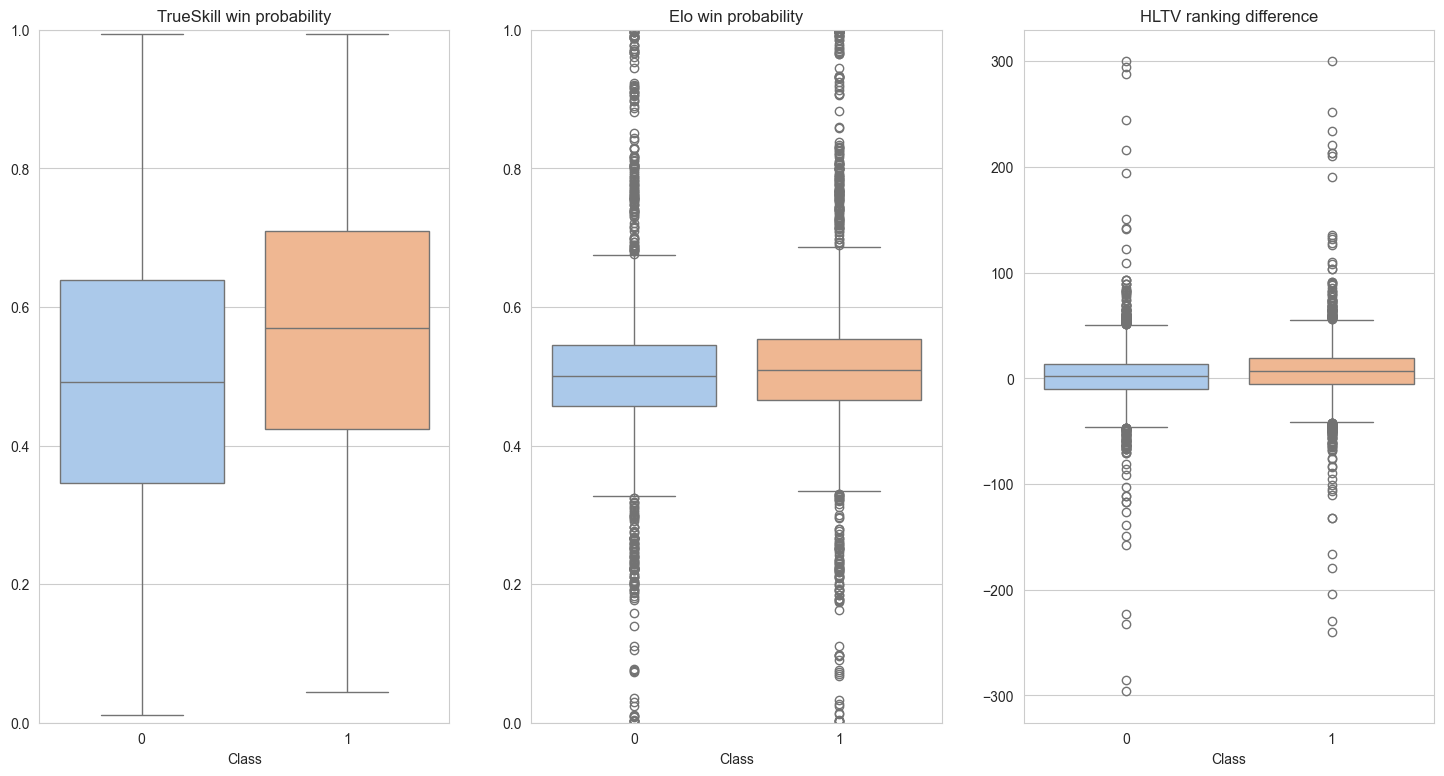
\includegraphics[width=1.2\textwidth]{Figures/class-box-new-1.png}
	\end{adjustbox}
	\caption{Boxplot of 'TrueSkill win probability', 'ELO win probability', and 'HLTV ranking difference' for either class}
	\label{fig:win_prob_class_dist}
\end{figure}

A similar trend is observed in Figure \ref{fig:win_rate_class_dist}, which plots the distribution of various win rates. The winning team generally had a higher overall win-rate for prior matches. The number of maps where a team had a higher win-rate can range from -7 to 7 (as there are seven maps in the competitive map pool). The median value was 1 indicating that the winning team usually had at least one more map with a higher win-rate than their opponent. The head-to-head historical map win-rate feature is also interesting, as there is a higher disparity between the classes. The conclusion that can be drawn here is that if team $x$ beat team $y$ more often than not in the past, they will likely continue to beat them in future. The IQR was, however, quite broad. Furthermore, for over 60\% of the matches, both teams had not played each other in the last 3 months.

\begin{figure}[h]
	\centering
	\begin{adjustbox}{center}
		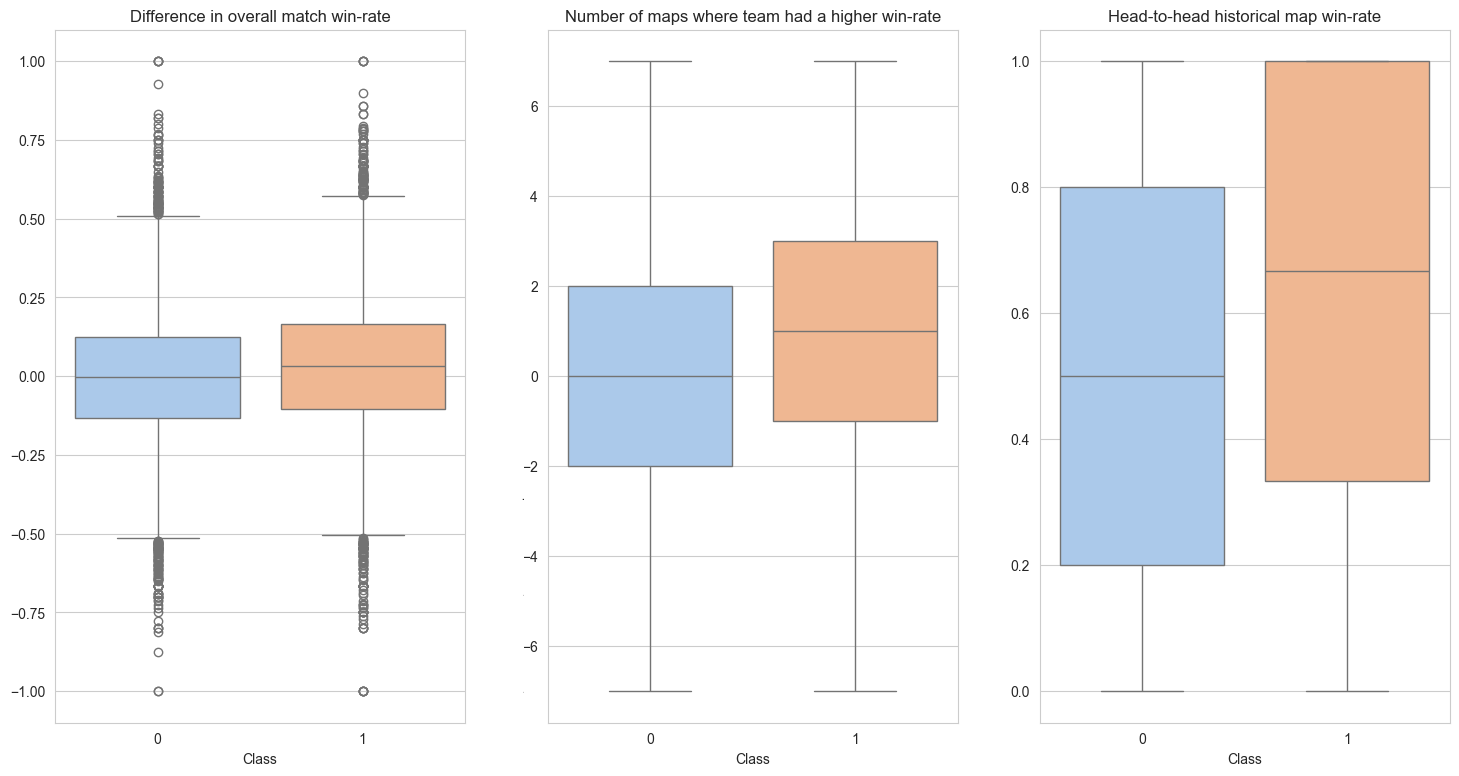
\includegraphics[width=1.2\textwidth]{Figures/class-box-new-2.png}
	\end{adjustbox}
	\caption{Boxplot of 'difference in match win-rate', 'maps with a higher win-rate', and 'head-to-head historical map win-rate' for either class}
	\label{fig:win_rate_class_dist}
\end{figure}

The most popular format in the dataset is BO3, with \matchesBoThree{} matches played (78.5\%). There were a further \matchesBoOne{} BO1s and \matchesBoFive{} BO5s played. The remaining 47 matches were played in BO2 maps, a format used briefly for lower-level league matches in 2019 and never again since. 

\matchesLAN{} (19.7\%) of the matches were played in a LAN environment, with the other \matchesOnline{} (80.3\%) being played online. 

Shortly after its release in September 2023, the professional scene transitioned to CS2. This meant that only \matchesCSTwo{} matches in the database were played in the new game, with the vast majority (\matchesCSGO{}) played in CS:GO. As the dataset grows in future, the proportion will shift in favour of CS2 matches. Nevertheless, the core game has remained unchanged, and the same analysis is applicable for both iterations of Counter-Strike.

\newpage

\subsection{Feature correlation}

It is useful to plot a correlation matrix to understand the relationships between pairs of variables. It can also help to identify multicollinearity, where independent variables are highly correlated. Highly correlated features essentially provide redundant information to a model, and can result in unstable and unreliable coefficient estimates. Dimensionality reduction techniques, such as principal component analysis, can be implemented to mitigate multicollinearity, however with the trade-off that new uncorrelated variables, called principal components, are less interpretable.

The correlation matrix for thirty of the features is plotted in Figure \ref{fig:corr}. It is immediately observable that none of the features correlate strongly with the target class \textit{win}. This is evident by the top row consisting of just pale colours. 

\begin{figure}[h]
	\centering
	\begin{adjustbox}{center} % Center the table
		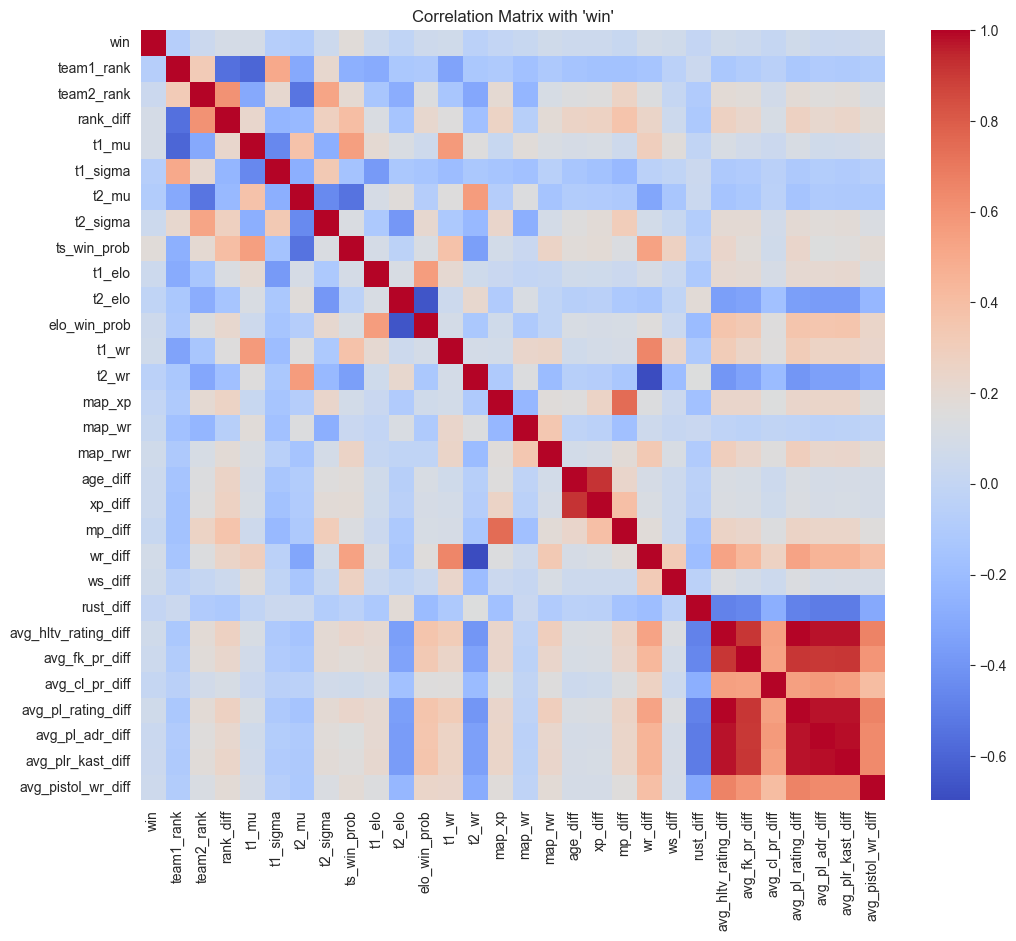
\includegraphics[width=1.3\textwidth]{Figures/corr-plot.png}
	\end{adjustbox}
	\caption{Feature correlation matrix heat-map}
	\label{fig:corr}
\end{figure}

\clearpage

A negative correlation between `team1\_rank' and 't1\_mu' exists, as well as for 'team2\_rank' and 't2\_mu'. This is a good indication that the TrueSkill system was implemented correctly. The best teams are ranked ascending from 1st, 2nd, 3rd - it is logical for teams with a low rank value to have a higher TrueSkill average ($\mu$). The TrueSkill averages correlate with their respective match win-rates.

Lineup age (measured in days) and experience (measured in number of matches together) also exhibit an unsurprising correlation. 

The red cluster in the bottom-right indicates a strong correlation between the  performance features. This is not too surprising because generally, having a high ADR or KAST will lead to a higher player rating, and having higher player ratings leads to a higher team rating. Furthermore, the more 'clutches' and 'first kills' obtained per round, the higher your team's overall performance will be.

% The number of maps and matches played each month and year
% distribution of match format (best of 1/2/3/5)
% distribution of maps played (mirage/inferno/etc)
% number of matches played by rank
% distribution of scores (13-0, 13-1, 13-2, 13-3, etc)
% score distribution and subsequent probability of winning (1-0, 2-0, 2-1, 3-1, 3-2, 4-0, 4-1, 4-2, 4-3, etc.)
% number of events, online/LAN, prizepools
% 1st pistol round win and map win (split by T/CT)
% 2nd pistol round win given each permutation of first half-score (split by T/CT)
% After winning opponent’s map pick, probability of winning series
% After winning your map pick, probability of winning series
% Matches won with rank differential

\subsection{Baseline model predictors}

\label{feature-selection}

It is useful to evaluate the performance of more basic models, with only 1 or 2 features, to form a baseline benchmark with which comparisons can be made. This will help to understand if the use of machine learning techniques offers a real benefit over a simpler analysis. To facilitate this, the most important features were identified via a feature selection process.

\textit{Feature selection} refers to the selection of the most relevant features from a dataset. It is used to reduce over-fitting and simplify models. Features can be selected either based on a statistical measure (a filter method), or by evaluating the performance of models using different subsets of features (a wrapper method).

A filter method was implemented using the \texttt{\textbf{f\_classif}} function from scikit-learn's \texttt{\textbf{feature\_selection}} class. By computing the ANOVA F-value, or \textit{F-statistic}, between each feature and the target class, each feature can be ranked and compared. The ANOVA F-value refers to the ratio of variance between the classes and the variance within the classes for each feature, thereby determining how well each feature can discriminate between each class, $y=0$ or $y=1$. If a feature has a higher ANOVA F-value, it has a stronger relationship with the target class and is potentially more useful for classification.

Other methods for feature selection were considered, such as \texttt{\textbf{SelectFdr}} which accounts for the family-wise error rate. However given the exploratory data analysis context, the filter method was deemed sufficient, and the best $k$ features or top $n^{th}$ percentile were identified using the \texttt{\textbf{SelectKBest}} function. The information presented in Figure \ref{fig:f-stat} was obtained by setting $k = 15$. 
\clearpage

\begin{figure}[h]
	\centering
	\begin{adjustbox}{center} % Center the table
		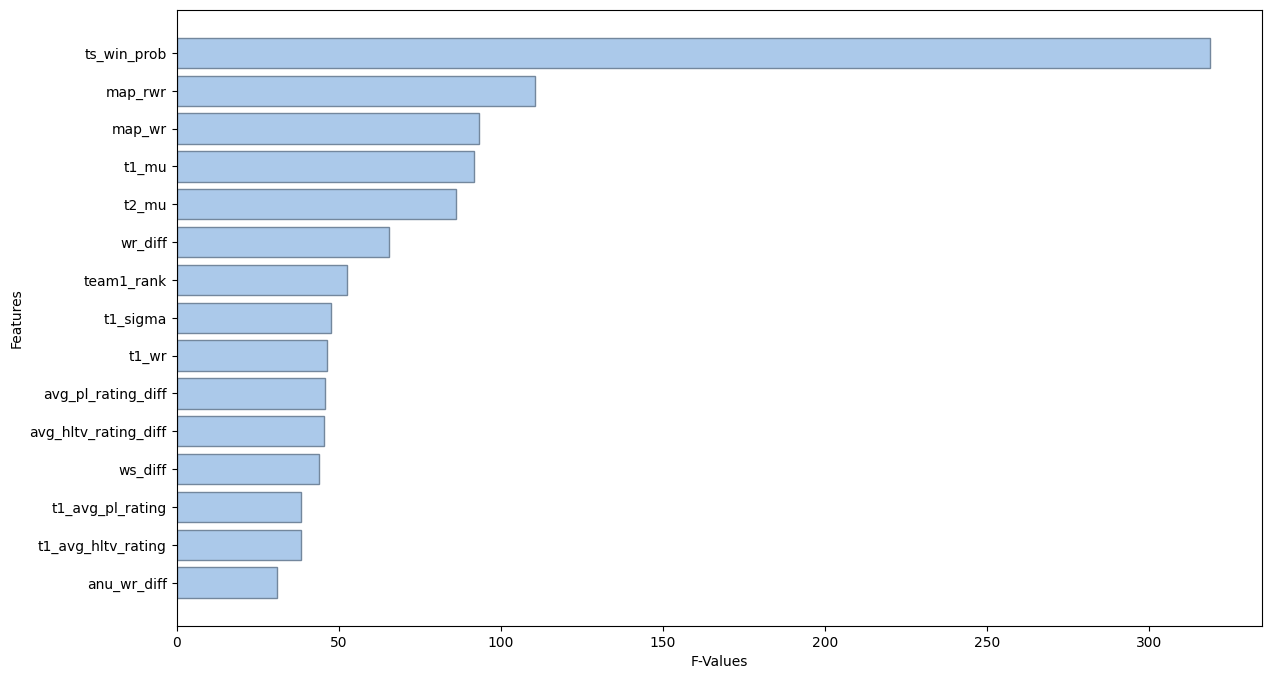
\includegraphics[width=1.3\textwidth]{Figures/f-statistik.png}
	\end{adjustbox}
	\caption{Barplot of best features by F-value}
	\label{fig:f-stat}
\end{figure}

The TrueSkill features appear to be the best predictors of the match outcome, with the win probability and mean $\mu$ values for either team exhibiting the highest scores. The map win-rate differential, round win-rate differential, and HLTV world ranking all follow, but with a large drop-off in score.

From these insights, we can establish three baseline models:

\begin{enumerate}
	\item the TrueSkill win probability model
	\item the HLTV world ranking model, where the team with the higher rank is always predicted to win
	\item the map win-rate model, where the team with the higher win-rate on more maps is always predicted to win. If both teams are equal, then the team with the higher overall round win-rate on more maps is predicted to win.
\end{enumerate}

\textbf{TrueSkill} achieved a classification accuracy of 57.00\% on the full dataset of \matchesTotal{} matches. The confusion matrix is shown in Table \ref{tab:ts-conf}. 

From the matrix, a number of useful statistics can be computed. The true positive rate (TPR, also known as sensitivity or recall) is the proportion of actual positives correctly identified by the model. The true negative rate (TNR, also known as specificity) is the proportion of actual negatives correctly identified by the model. Precision refers to the proportion of positive classifications that were correct. The F1-score is a balanced measure of precision and recall. These metrics will be discussed in more depth later. The TrueSkill model achieved a true positive rate of 0.62, a true negative rate of 0.516, a precision of 0.58, and a F1-score of 0.60.

\begin{table}[h]
	\centering
	\begin{tabular}{c|c|c|}
		\cline{2-3}
		& \textbf{Predicted: No} & \textbf{Predicted: Yes} \\ \hline
		\multicolumn{1}{|c|}{\textbf{Actual: No}} & 2516 & 2363 \\ \hline
		\multicolumn{1}{|c|}{\textbf{Actual: Yes}} & 1999 & 3267 \\ \hline
	\end{tabular}
	\caption{Confusion matrix for the TrueSkill model}
	\label{tab:ts-conf}
\end{table}

TrueSkill can evaluate the probability of a team winning, which means a receiver operating characteristic curve can be constructed by varying the threshold at which this probability is enough to make a positive classification. The area under the receiver operating characteristic curve (AUC ROC) is a measure of classifier's ability to distinguish between the two classes. As shown in Figure \ref{fig:ts-roc}, the TrueSkill model is indeed a better predictor than random chance, with the area under the curve, $AUC = 0.5997$. The probabilities generated by TrueSkill may also be converted into betting odds. This aspect will be discussed later.
 
\begin{figure}[h]
	\centering
	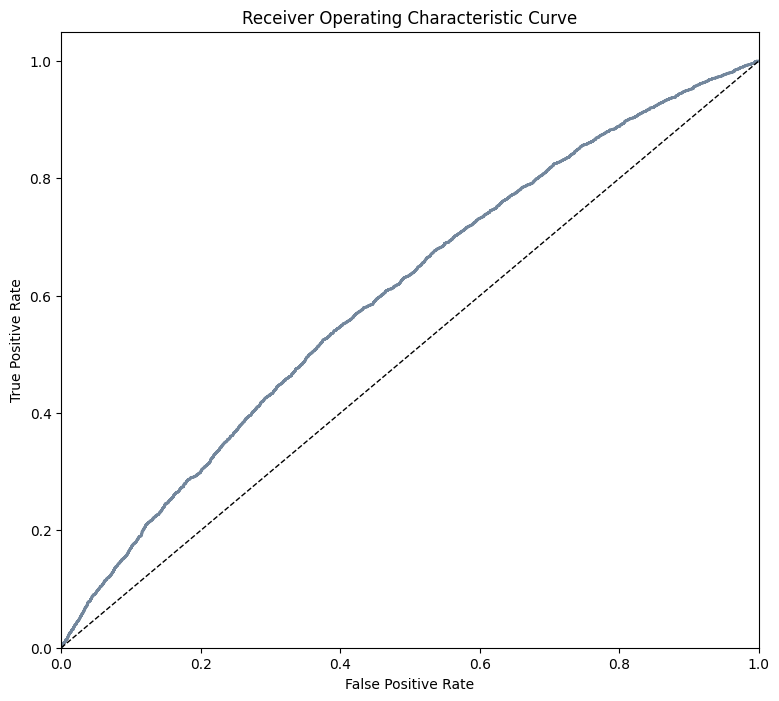
\includegraphics[width=\textwidth]{Figures/ts-auc.png}
	\caption{ROC curve for the TrueSkill model}
	\label{fig:ts-roc}
\end{figure}

The \textbf{HLTV world ranking model}, which assumes the higher-ranked team will always win the match, correctly classified the winner for 56.28\% of the matches, achieving a slightly higher F1-score than TrueSkill of 0.61. The final baseline model, the \textbf{map win-rate model}, achieved only 54.95\% classification accuracy and a lower F1-score of 0.579. As neither of these last two models produce classification probabilities, no receiver operating characteristic curve can be constructed.

\section{Modelling}

After considering the methods used in the literature, the following supervised learning models were selected and trained to predict the match winner:

\begin{itemize}
	\item Logistic regression
	\item Random forests
	\item Support vector machine
	\item $k$-nearest neighbours
	\item Gaussian Naive Bayes
	\item Multilayer perceptron
	\item XGBoost
\end{itemize}

\subsection{Data segmentation}

To accurately assess the performance of any ML model, it must be tested on data which has not been used during training. The data should therefore be split into a training set and a testing set. Because the match data is chronological time-series data, it would not be appropriate to randomise the data prior to splitting, which is a common practice. It is more appropriate to segment the data chronologically.

A portion of the earliest match data was excluded from both training and testing. These matches were used to generate features for the later matches. This served two main purposes: the initialisation of Elo and TrueSkill ratings, and for providing historical data for most of the match- and performance-history features. This initialisation set amounted to the first 10\% of the dataset, which was 1127 matches spanning a period of five months. This ensured that the features generated for the first match in the training set could draw upon accurate player ratings and sufficient match history for each team.

The remaining 90\% of the data shall henceforth be referred to as the \textit{full dataset}. It was split with a ratio of 80:20 for the training and testing sets. The test set consisted of every match played in 2023. This amounted to 8116 match records for training and 2029 for testing.

Filters were later applied to the full dataset in order to identify if certain types of matches were easier to predict than others. The different scenarios tested were:
\begin{enumerate}
	\item the full dataset,
	\item a dataset which excluded all Best-of-1 (single map) matches,
	\item a dataset which excluded matches without a team ranked in the Top-30,
	\item a dataset which excluded matches without a team ranked in the Top-15, and
	\item a dataset which excluded all matches which were played online (i.e. LAN matches only)
\end{enumerate}

The same process was performed for each dataset: data segmentation, feature scaling, feature selection, hyperparameter tuning, and performance evaluation.

\subsection{Feature scaling}

Some models, such as those which use gradient descent for optimisation, are sensitive to the magnitude of features. This means that each numeric feature should be \textit{scaled} prior to training. There are two methods of scaling features, namely \textit{normalisation} and \textit{standardisation}. In normalisation, each feature is scaled to fit into the range $[0, 1]$ by subtracting the minimum value and dividing by the range, ($max-min$). Although normalised data preserves the distribution of the original data, it is more sensitive to outliers. 

In standardisation, the data is transformed to have a zero mean and unit variance using the familiar equation:

\[ z_i = \frac{x_i-\mu}{\sigma} \]

Where $z_i$ is the new value, $x_i$ is the original value, $\mu$ and $\sigma$ are the mean and standard deviation of $x$.

Both techniques were implemented using the \texttt{\textbf{MinMaxScaler}} and \texttt{\textbf{StandardScaler}} classes from scikit-learn. During testing, it was found that normalisation degraded model performance significantly when compared to both the unscaled and standardised data. This is because normalisation is sensitive to outliers, which were present in many of the features. It was therefore decided to scale the features using standardisation. 

\subsection{Hyperparameter tuning}

Each ML model has configuration settings which dictate the structure and computational performance of the model. These settings are known as \textit{hyperparameters}. An example of a hyperparameter is the maximum depth of the decision trees used in random forests, or the choice of kernel used in a SVM.

When tuning these parameters to find the optimal configuration, it is a good practice to partition a portion of the training set into a validation set. The performance of models with different configurations can be compared by testing them on the validation set.

A technique known as $k$-fold cross-validation splits the training data into $k$ folds (partitions). The training is then performed repeatedly with a different fold used as the validation set for each iteration. This approach provides a proxy for estimating the out-of-sample performance, ensuring that a balanced measure of performance is attained for each configuration of hyperparameters.

The \texttt{\textbf{GridSearchCV}} class from scikit-learn was utilized to test several different hyperparameters grids (configurations) using $k$-fold cross-validation. For many of the hyperparameters, a broad initial range of values was used. This range was progressively narrowed down in an iterative process until the configuration yielding the greatest average classification accuracy on the validation set was found.

The hyperparameters for each method and the range of values considered are explained in the following subsections.

\subsubsection{Logistic regression}

Table \ref{tab:lr_params} presents the hyperparameters of the logistic regression model and the respective ranges of values explored during the tuning process.

\begin{table}[h]
	\centering
	\begin{tabular}{ll}
		\toprule
		\multicolumn{1}{c}{\textbf{Hyperparameter}} & \multicolumn{1}{c}{\textbf{Values Tested}} \\
		\midrule
		1/Regularisation strength (C)              & $10^{-5}$ - $10^{2}$ \\
		Regularisation type                       & None, L1 (Lasso), L2 (Ridge) \\
		Solver                                    & liblinear, lbfgs, saga \\
		\bottomrule
	\end{tabular}
	\caption{Logistic regression hyperparameters and the range of values tested}
	\label{tab:lr_params}
\end{table}

Regularisation introduces a penalty term to the loss function which helps control the size of the coefficients. This can mitigate the risk of overfitting by preventing the model from relying too heavily on any single predictor variable. There are two \textit{types} of regularisation, Lasso and Ridge.

$C$ is the inverse of the \textit{regularisation strength} parameter $\lambda$. Higher values of $C$ therefore correspond to less regularisation, while lower values enforce stronger regularisation.

The \textit{solver} is the algorithm used to minimise the loss function. 

\subsubsection{Random forests}

Table \ref{tab:rf_params} presents the hyperparameters of the random forests model and the respective ranges of values used in the tuning process.

\begin{table}[h]
	\centering
	\begin{tabular}{ll}
		\toprule
		\multicolumn{1}{c}{\textbf{Hyperparameter}} & \multicolumn{1}{c}{\textbf{Values Tested}} \\
		\midrule
		Number of estimators       & 20 - 500 \\
		Maximum depth              & 2 - None \\
		Minimum samples for split  & 2 - 10 \\
		Minimum samples per leaf   & 1 - 10 \\
		Maximum features           & 1 - None \\
		\bottomrule
	\end{tabular}
	\caption{Random forests hyperparameters and the range of values tested}
	\label{tab:rf_params}
\end{table}

The \textit{number of estimators} is the number of decision trees to include in the ensemble. Increasing this value can improve performance but also increases computational cost.

The \textit{maximum depth} limits the maximum depth of each decision tree. Deeper trees can capture more complex relationships but may overfit the data. 

The \textit{minimum samples for split} are the amount of samples needed at a node in order to split it further. The \textit{minimum samples per leaf} are the lowest amount of samples that can exist at a leaf node. The greater these values, the simpler the trees become.

The \textit{maximum features} refers to the maximum amount of features considered when looking for the best split. Limiting the number of features reduces the risk of overfitting.

\subsubsection{Support vector machine}

Table \ref{tab:svc_params} presents the hyperparameters of the support vector machine and the respective ranges of values explored during the tuning process.

\begin{table}[h]
	\centering
	\begin{tabular}{ll}
		\toprule
		\multicolumn{1}{c}{\textbf{Hyperparameter}} & \multicolumn{1}{c}{\textbf{Values Tested}} \\
		\midrule
		Kernel                     & 'linear', 'poly', 'rbf', 'sigmoid' \\
		Regularisation (C)         & $10^{-3}$ - $10^{3}$ \\
		Degree (for 'poly' kernel) & 2 - 5 \\
		Gamma (for 'rbf' kernel)   & $10^{-5}$ - $10^{0}$ \\
		\bottomrule
	\end{tabular}
	\caption{Support Vector Classifier hyperparameters and the range of values tested}
	\label{tab:svc_params}
\end{table}

The \textit{kernel} function defines the shape of the decision boundary.

For a support vector classifier, Ridge regularisation is implemented by means of a penalty term for the complexity of the decision boundary. The \textit{regularisation} parameter C is the inverse of the strength of regularisation, where lower values of C correspond to stronger regularisation, while higher values correspond to weaker regularisation

For the polynomial kernel, the \textit{degree} specifies the polynomial order, and for the RBF kernel, the \textit{gamma} parameter defines the kernel width.

\subsubsection{\textit{k}-nearest neighbours}
Table \ref{tab:knn_params} presents the hyperparameters of the $k$-nearest neighbours classifier and the respective ranges of values explored during the tuning process.

\begin{table}[h]
	\centering
	\begin{tabular}{ll}
		\toprule
		\multicolumn{1}{c}{\textbf{Hyperparameter}} & \multicolumn{1}{c}{\textbf{Values Tested}} \\
		\midrule
		Number of neighbours			   & 1 - 30 \\
		Weight function			           & 'uniform', 'distance' \\
		Algorithm                          & 'auto' \\
		Power parameter (p)                & 1 - 2 \\
		\bottomrule
	\end{tabular}
	\caption{$k$-nearest neighbours hyperparameters and the range of values tested}
	\label{tab:knn_params}
\end{table}

The \textit{number of neighbours} are the number of neighbouring data points which are considered for classification. A higher value can reduce noise but may also smooth out decision boundaries.

The \textit{weight function} assigns a weight to each neighbour based on its distance from the query point. 'uniform' gives equal weight to all neighbours, while 'distance' weights closer neighbours more heavily.

The \textit{algorithm} parameter specifies the algorithm used for computing nearest neighbors. 'auto' selects the best approach based on the dataset.

The \textit{power} parameter (p) is used for the Minkowski metric, which calculates the distance between data points. The Manhattan distance is used when $p=1$, and the Euclidean distance is used when $p=2$.

\subsubsection{Gaussian Naive Bayes}

The Gaussian Naive Bayes classifier is a relatively simple model and has only a single hyperparameter, \textit{var\_smoothing}, which is a small positive value added to the variance of each Gaussian used in the model. Adding this smoothing value can prevent numerical instabilities if the variance of a feature approaches 0. The range of values tested was $10^{-10}$ - $10^{-5}$.

\subsubsection{Multilayer perceptron}

Table \ref{tab:mlp_params} presents the hyperparameters of the MLP classifier and the respective ranges of values explored during the tuning process.

\begin{table}[h]
	\centering
	\begin{tabular}{ll}
		\toprule
		\multicolumn{1}{c}{\textbf{Hyperparameter}} & \multicolumn{1}{c}{\textbf{Values Tested}} \\
		\midrule
		Hidden layer sizes  				& \textit{see below} \\
		Activation function 				& 'identity', 'logistic', 'tanh', 'relu' \\
		Solver 								& 'lbfgs', 'sgd', 'adam' \\
		Learning rate 						& 'constant', 'invscaling', 'adaptive' \\
		Alpha 								& 0.0001, 0.001, 0.01, 0.1 \\
		Batch size 							& 'auto', 20 - 400 \\
		Max iterations					    & 200 - 10000 \\
		\bottomrule
	\end{tabular}
	\caption{Multilayer perceptron hyperparameters and the range of values tested}
	\label{tab:mlp_params}
\end{table}

The \textit{hidden layer sizes} are the number of neurons in each hidden layer. Different configurations of hidden layers can affect the model's ability to capture complex patterns. The hidden-layer topologies tested include wide (200,200), narrow (20,20), bottleneck (200, 50, 200), and hierarchical (200, 100, 50). The amount of neurons in each hidden layer in each topology was varied from 1 to 400. The maximum number of hidden layers tested was five.

The \textit{activation function} defines the function used for activating neurons in the hidden layers, where 'identity' is a linear activation, 'logistic' is the sigmoid function, 'tanh' is the hyperbolic tangent, and 'relu' is the rectified linear unit.

The \textit{solver} is the optimization algorithm used to update the weights. 'lbfgs' is an quasi-Newton method, 'sgd' is stochastic gradient descent, and 'adam' is a stochastic gradient-based optimizer.

The \textit{learning rate} controls the step size used when updating the weights. 'constant' uses a fixed learning rate (0.001), 'invscaling' gradually decreases the learning rate, and 'adaptive' maintains the learning rate unless the training loss ceases to improve.

The \textit{alpha} parameter is the regularisation term, similar to $\lambda$ in logistic regression and SVMs.

The \textit{batch size} is the number of samples processed before the model is updated. Smaller batch sizes allow the model to learn faster but can be more unstable, while larger batch sizes provide more stable updates but may take longer to converge.

The \textit{max iterations} parameter is the maximum number of iterations the solver will run for. This allows "early stopping" if convergence is not reached after max\_iter. For stochastic solvers (‘sgd’, ‘adam’), this is the number of times each data point is used (epochs).

\subsubsection{XGBoost}
Table \ref{tab:xgb_params} presents the hyperparameters of the XGBoost classifier and the respective ranges of values explored during the tuning process.

\begin{table}[h]
	\centering
	\begin{tabular}{ll}
		\toprule
		\multicolumn{1}{c}{\textbf{Hyperparameter}} & \multicolumn{1}{c}{\textbf{Values Tested}} \\
		\midrule
		Number of estimators	  				  & 50 - 10000 \\
		Learning rate        					  & 0.001, 0.01, 0.1, 0.2, 0.3 \\
		Max depth            					  & 2 - 10 \\
		Subsample 								  & 0.5 - 1.0 \\
		Colsample by tree 					 	  & 0.5 - 1.0 \\
		Gamma 									  & 0, 0.1, 0.2, 0.3 \\
		\bottomrule
	\end{tabular}
	\caption{XGBoost hyperparameters and the range of values tested}
	\label{tab:xgb_params}
\end{table}

The \textit{number of estimators} is the number of trees in the model. More trees can increase the model's performance but also the risk of overfitting.

The \textit{learning rate} (eta) controls the step size at each iteration while minimising the loss function. Lower learning rates make the model more robust to overfitting by shrinking the feature weights.

The \textit{max depth} parameter defines the maximum depth of a tree. Deeper trees can model more complex relationships but are more prone to overfitting.

The \textit{subsample} parameter is the fraction of samples to be used for fitting each tree, while \textit{colsample by tree} is the fraction of features to be used for each tree. These parameters prevent overfitting by adding randomness.

The \textit{gamma} parameter specifies the minimum reduction in loss needed to split a node, thereby controlling the complexity of the trees.
 
\subsection{Performance evaluation}

Once each model has been trained, each match in the test set is classified into either class, $y=1$ (team 1 wins), or $y=0$ (team 1 loses, i.e. team 2 wins). 

The classification accuracy refers to the percentage of matches that was correctly classified by each model. It is reported as \textbf{Test ACC} in the results tables in the following chapter. 

\textbf{Precision} is a measure of the accuracy of positive predictions. It is the percentage of matches that were actually won out of the set of positive predictions. \textbf{Recall}, also known as sensitivity, measures the proportion of true positives that are correctly classified by the model.

\[ \text{Precision} = \frac{\text{True Positives}}{\text{True Positives} + \text{False Positives}} \]
\[ \text{Recall} = \frac{\text{True Positives}}{\text{True Positives} + \text{False Negatives}} \]

\textbf{F1-score} is another measure of predictive performance which balances both precision and recall. 

\[ F_1 = \frac{2 \times precision \times recall}{precision + recall} \]

Finally, the \textbf{area under receiver operating characteristic curve} (AUC ROC) is a measurement of the classification performance of a model at different threshold settings. The ROC curve plots the True Positive Rate (recall) against the False Positive Rate as the discrimination threshold is varied from 0 to 1. A random classifier will therefore, on average, have a straight line from (0,0) to (1,1) with a corresponding AUC ROC of 0.5. An AUC ROC of 1.0 indicates that the model can perfectly distinguish the positive and negative classes.

\subsection{Betting odds generation}

Each of the models generate the probability $p(y)$ of an observation belonging to each class. These probabilities are then used to generate the betting odds. Odds can be represented in a number of ways. For this research, all odds are denoted as decimal odds, which is a decimal number representing the payout per unit wagered. 

The decimal odds are the reciprocal of the probability of the event occurring as shown in the following equation:

\[ \left( O_A, O_B \right)  = \left( \frac{1}{p(y=1)}, \frac{1}{p(y=0)} \right) \]

Where $O_A$ and $O_B$ are the decimal odds for team A and B to win the match, and $p(y)$ is the probability of team A winning $(y=1)$ or team B winning $(y=0)$. In practice, these odds represent the \textit{fair} odds which exclude the effect of the bookmaker margin: a reduction in the decimal odds to increase bookmaker profitability.

\newcommand{\matchesBet}{347}
\newcommand{\tournamentsBet}{11}

\subsection{Betting odds evaluation}

In order to compare the generated betting odds with real betting odds provided by bookmakers, the average odds for \matchesBet{} matches across \tournamentsBet{} tournaments in the test set (2023) were downloaded from an online archive at \texttt{oddsportal.com}. To remove the bookmaker margin, the odds were then converted back into probabilities and normalized such that the sum of each pair of probabilities added up to 1.

The correlation, mean absolute error (MAE), and root mean square error (RMSE) between the generated odds and the bookmaker odds is reported for each model to quantify the discrepancy between the odds from the models and the bookmaker. These are formulated as follows:\label{bettingstats}

Given that the generated odds are $O_g$ and the bookmaker odds are $O_b$, with $n$ being the total number of odds comparisons, the \textbf{correlation} is defined as:

\[r = \frac{\sum_{i=1}^{n} (O_{g_i} - \bar{O_g})(O_{b_i} - \bar{O_b})}{\sqrt{\sum_{i=1}^{n} (O_{g_i} - \bar{O_g})^2 \sum_{i=1}^{n} (O_{b_i} - \bar{O_b})^2}}\]

where:
\begin{itemize}
	\item $O_{g_i}$ and $O_{b_i}$ are the i-th generated and bookmaker odds, respectively.
	\item $\bar{O_g}$ and $\bar{O_b}$ are the means of the generated and bookmaker odds.
\end{itemize}

The \textbf{mean absolute error} (MAE) is defined as:
\[\text{MAE} = \frac{1}{n} \sum_{i=1}^{n} |O_{g_i} - O_{b_i}|\]

And finally, the \textbf{root mean square error} (RMSE) is defined as
\[\text{RMSE} = \sqrt{\frac{1}{n} \sum_{i=1}^{n} (O_{g_i} - O_{b_i})^2}\]

\subsection{Betting simulation}

Finally, a betting simulation was performed to test each model's real-world performance using the following basic strategy: the bookmaker odds for each match was first converted into a probability. If the model generated a higher probability for either team to win than what was offered by the bookmaker, a one unit bet was placed on that team. 

For example, consider a scenario where the bookmaker odds for team A : team B is 1.28~:~3.36. These odds correspond to $p(y=1)=0.78$ and $p(y=0)=0.30$ (the sum is greater than 1 because of the bookmaker margin).

If the model then predicts that $p(y=1)=0.65$ and $p(y=0)=0.35$ for this match, it would place a one unit bet on team B, despite it having a lower probability of winning. 

On the other hand, if it had generated $p(y=1)=0.75$ and $p(y=0)=0.25$, it has determined that neither team is worth betting on.

The proportion of matches bet on, win-percentage, loss-percentage, and resulting profit or loss for each model is reported in the Results. 
\chapter{Results and Discussion}
\label{Results}

\section{Model Performance}

The performance of each machine learning model is reported under different circumstances. Filters were applied to the dataset in order to identify if certain types of matches were easier to predict than others. The different scenarios tested were:
\begin{enumerate}
	\item the full dataset which includes all matches
	\item the full dataset using selected features
	\item a dataset which excluded Best-of-1 matches
	\item a dataset which excluded matches without a team ranked in the Top-30
	\item a dataset which excluded matches without a team ranked in the Top-15
	\item a dataset which excluded all matches played online
\end{enumerate}

All figures reported in the tables to follow are percentages, unless specified otherwise. The best result achieved in each category is highlighted in \textbf{bold}.

\subsection{Full dataset}

The first scenario entailed training each model using all 142 features. The full dataset consists of 10145 matches, with 8116 used for training and 2029 for testing. The results obtained for this setup are tabulated in Table \ref{table:1}. The precision, recall, F1 score, and ROC AUC scores were obtained for the test set.

\begin{table}[h!]
	\centering
	\small
	\begin{adjustbox}{center} % Center the table
		\begin{tabular}{ |l|c|c|c|c|c|c| }
			\hline
			\rule{0pt}{2.6ex} \textbf{Model} & \textbf{Train ACC} & \textbf{Test ACC} & \textbf{Precision} & \textbf{Recall} & \textbf{F1 Score} & \textbf{ROC AUC} \\
			\hline
			\rule{0pt}{2.6ex} TrueSkill                 & 56.8 & 57.9 & 57.2 & 62.4 & 59.7 & 61.6 \\ \hline
			\rule{0pt}{2.6ex} Logistic Regression 		& 60.0 & 58.5 & 56.9 & 69.3 & 62.5 & 62.9 \\
			\rule{0pt}{2.6ex} Random Forest 			& 64.3 & 58.3 & 56.7 & 69.9 & 62.6 & 62.5 \\
			\rule{0pt}{2.6ex} Support Vector Machine 	& 59.5 & 59.4 & \textbf{58.3} & 66.3 & 62.0 & 63.0 \\
			\rule{0pt}{2.6ex} XGBoost 					& 61.0 & \textbf{60.0} & \textbf{58.5} &\textbf{ 69.6} & \textbf{63.5} & \textbf{64.1} \\
			\rule{0pt}{2.6ex} Gaussian Naive Bayes 		& 56.6 & 55.7 & 57.4 & 44.5 & 50.1 & 59.0 \\
			\rule{0pt}{2.6ex} MLP Neural Network 		& 59.9 & 59.7 & 59.0 & 63.8 & 61.3 & 62.1 \\
			\rule{0pt}{2.6ex} k-Nearest Neighbours 		& 58.9 & 55.9 & 55.3 & 61.2 & 58.1 & 57.8 \\
			\hline
		\end{tabular}
	\end{adjustbox}
	\caption{Performance of ML models trained with all features on complete dataset}
	\label{table:1}
\end{table}

The machine learning models did not significantly outperform the TrueSkill baseline model, with the improvement in classification accuracy varying from -2\% to 2\%. XGBoost and MLP NN had the best overall performance with a classification accuracy of 60.0\% and 59.7\%  respectively. XGBoost had the highest recall, $F_1$ score, and AUC ROC, indicating slightly better ability to discriminate between classes.

The optimal set of hyperparameters for each model was found using grid search and is captured in Table \ref{table:hyperparameters} below.

 \begin{table}[h]
	\centering
	\small
	\begin{adjustbox}{center}
		\begin{tabular}{|l|l|l|}
			\hline
			\rule{0pt}{2.5ex}\textbf{Hyperparameter} & \textbf{Description} & \textbf{Value Selected} \\
			\hline
			\multicolumn{3}{|c|}{\rule{0pt}{2.5ex}\textit{Logistic Regression}} \\
			\hline
			C & Inverse of regularization strength & 0.01 \\
			penalty & Type of regularization & "l2" \\
			solver & Optimization algorithm & "liblinear" \\
			\hline
			\multicolumn{3}{|c|}{\rule{0pt}{2.5ex}\textit{Random Forest}} \\
			\hline
			n\_estimators & Number of trees in the forest & 100-400 \\
			max\_depth & Maximum depth of the tree & 2 \\
			min\_samples\_split & Min samples to split a node & 4 \\
			min\_samples\_leaf & Min samples to be at a leaf node & 4 \\
			max\_features & Number of features for best split & "log2" \\
			\hline
			\multicolumn{3}{|c|}{\rule{0pt}{2.5ex}\textit{Support Vector Machine}} \\
			\hline
			C & Regularization parameter & 0.1 \\
			kernel & Kernel type & "linear" \\
			gamma & Kernel coefficient & "scale" \\
			\hline
			\multicolumn{3}{|c|}{\rule{0pt}{2.5ex}\textit{XGBoost}} \\
			\hline
			n\_estimators & Number of gradient boosted trees & 208 \\
			learning\_rate & Step size shrinkage & 0.025 \\
			max\_depth & Maximum depth of a tree & 2 \\
			subsample & Subsample ratio of the training instances & 0.5 \\
			colsample\_bytree & Subsample ratio of columns for each tree & 0.5 \\
			gamma & Min loss reduction for partition on a leaf node & 0.1 \\
			\hline
			\multicolumn{3}{|c|}{\rule{0pt}{2.5ex}\textit{Gaussian Naive Bayes}} \\
			\hline
			var\_smoothing & Variance smoothing & 1e-9 \\
			\hline
			\multicolumn{3}{|c|}{\rule{0pt}{2.5ex}\textit{Multi-layer Perceptron}} \\
			\hline
			hidden\_layer\_sizes & Neurons in hidden layers & (5,4) \\
			activation & Activation function & "relu" \\
			solver & Solver for weight optimization & "sgd" \\
			alpha & L2 penalty (regularization term) & 0.001 \\
			learning\_rate & Learning rate for weight updates & "constant" \\
			\hline
			\multicolumn{3}{|c|}{\rule{0pt}{2.5ex}\textit{k-Nearest Neighbours}} \\
			\hline
			n\_neighbors & Number of neighbors to use & 110 \\
			weights & Weight function in prediction & "uniform", "distance" \\
			algorithm & Algorithm to compute nearest neighbors & "auto" \\
			p & Power parameter for Minkowski metric & 1 (Manhattan) \\
			\hline
		\end{tabular}
	\end{adjustbox}
	
	\caption{Hyperparameters and range of values tested for each ML model implemented}
	\label{table:hyperparameters2}
\end{table}

% LOG {'C': 0.01, 'penalty': 'l2', 'solver': 'liblinear'}
% RAN {'criterion': 'gini', 'max_depth': 5, 'max_features': 'log2', 'min_samples_leaf': 4, 'min_samples_split': 4, 'n_estimators': 300}
% SVM {'C': 0.1, 'gamma': 'scale', 'kernel': 'linear'}
% XGB {'learning_rate': 0.025, 'max_depth': 2, 'n_estimators': 200}
% GNV {'var_smoothing' : '1e-09'}
% MLP {'activation': 'relu', 'alpha': 0.001, 'hidden_layer_sizes': (10,100,10), 'learning_rate_init': 0.001, 'solver': 'sgd'}
% KNN {'n_neighbors': 110, 'p': 1, 'weights': 'uniform'}

As a consequence of the large number of features, the models were prone to overfit the training data. This was especially pronounced with random forests, XGBoost, and multilayer perceptron, which when initially configured could achieve near perfect accuracy on the training set, but otherwise performed poorly on the test set. In the case of random forests and XGBoost, this was mitigated by reducing the maximum depth of the trees to only 2 splits. For the MLP, the number of nodes per hidden layer had to be quite low (5,4) to avoid overfitting.

The weakest performers were $k$-Nearest Neighbours and Gaussian Naive Bayes, exhibiting worse performance than the TrueSkill base model.

The ROC curve for TrueSkill and the best performing ML model, XGBoost, are plotted in Figure \ref{fig:xgb-roc}. It is evident that both models are better at predicting match outcomes than random chance, however XGBoost is slightly superior with an AUC of 0.641 vs 0.624.

\begin{figure}[h]
	\centering
	\begin{adjustbox}{center}
		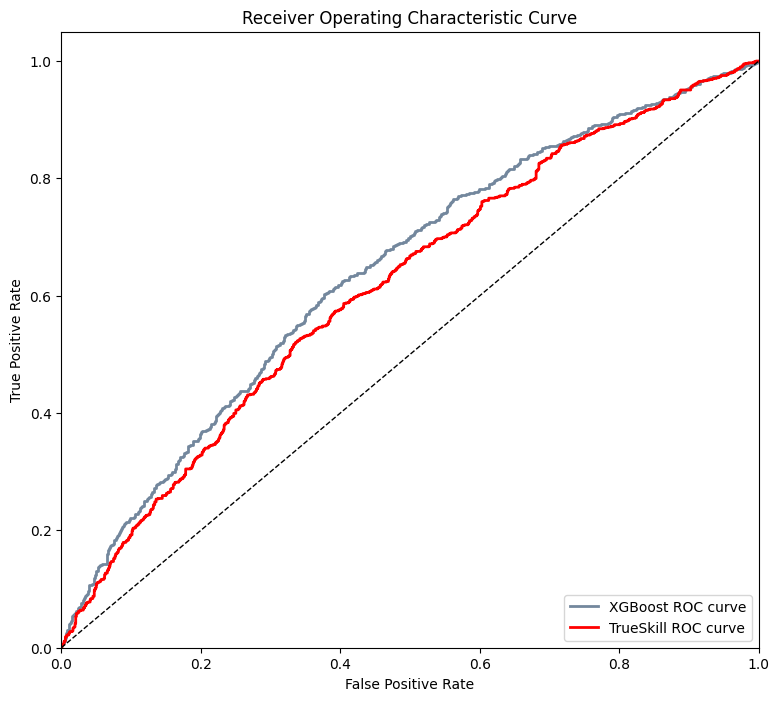
\includegraphics[width=1.1\textwidth]{Figures/xgb-auc.png}
	\end{adjustbox}
	\caption{Receiver operating characteristic curve for TrueSkill and XGBoost}
	\label{fig:xgb-roc}
\end{figure}

\subsubsection{Feature importance}

Feature selection methods such as filter and wrapper methods have already been discussed in Section \ref{feature-selection}. Some models can also be used to determine feature importance. In a regularised logistic regression model, the magnitude of the coefficients for each feature are indicative of their importance given a large enough regularization penalty. 

For SVMs with linear kernels, the weights assigned to each feature indicate their importance. With tree-based methods like random forests and XGBoost, the features yielding the largest average reduction in the loss function are more important. Figure \ref{fig:xgbimp} shows the feature importances determined by XGBoost.

\begin{figure}[h]
	\centering
	\begin{adjustbox}{center}
		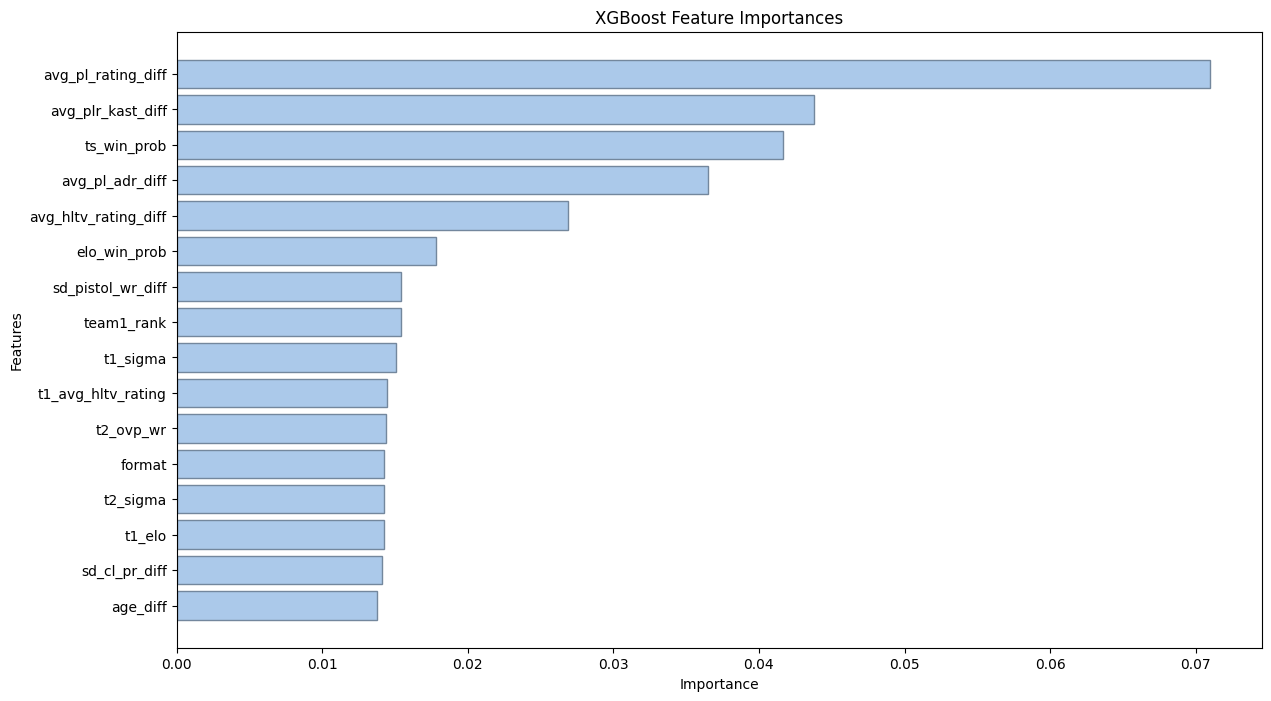
\includegraphics[width=1.3\textwidth]{Figures/xgb-imp.png}
	\end{adjustbox}
	\caption{Feature importance from XGBoost}
	\label{fig:xgbimp}
\end{figure}

In contrast to the filter methods in Section \ref{feature-selection}, XGBoost considers the difference in average player statistics (rating, KAST, ADR, and HLTV rating) between the two teams to be highly relevant measures. Both TrueSkill and Elo win probabilities are taken into account as well, whereas previously the Elo measure was discarded. 

With logistic regression, the feature importances differed considerably. As seen in Figure \ref{fig:logimp}, the TrueSkill win probability and $\mu,\sigma$ values for either team were very important, followed by the difference in average map win-rate, round win-rate per map. HLTV world ranking, and win-streak.

\clearpage

\begin{figure}[h]
	
	\centering
	\begin{adjustbox}{center} % Center the table
		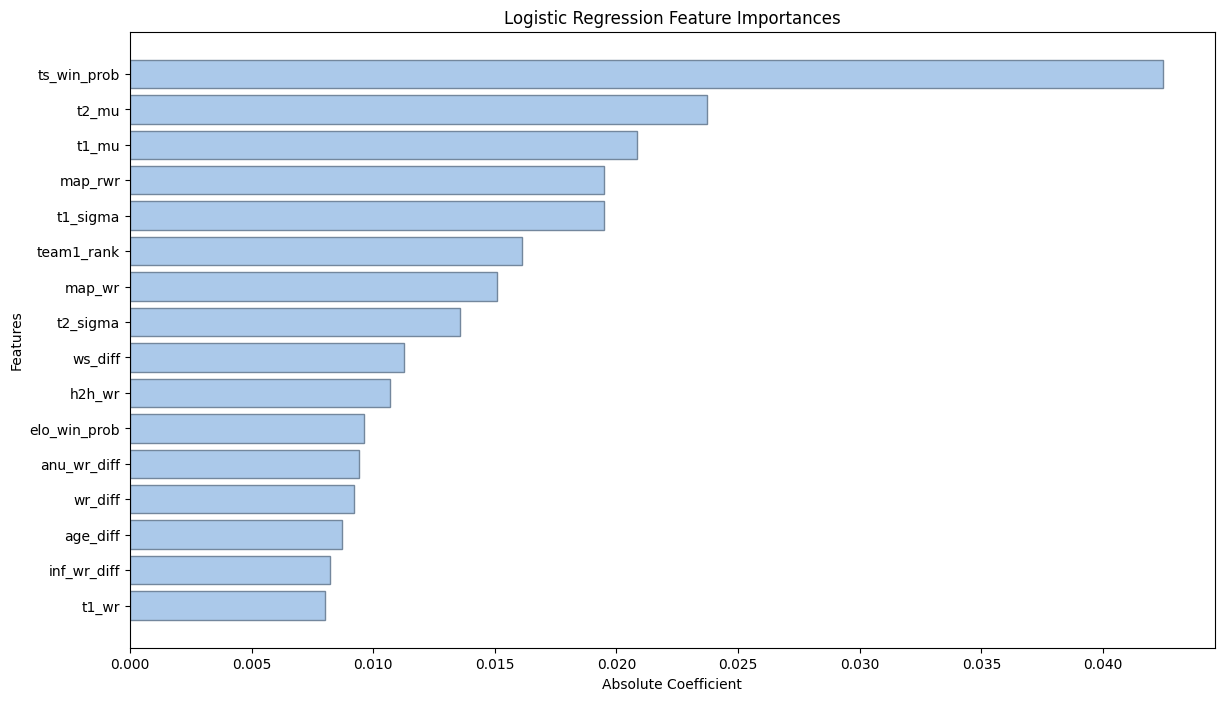
\includegraphics[width=1.3\textwidth]{Figures/logreg-imp.png}
	\end{adjustbox}
	\caption{Feature importance from logistic regression coefficients}
	\label{fig:logimp}
\end{figure}

\subsubsection{Performance using Feature Selection}

The results reported in Table \ref{table:2} below were obtained after reducing the number of features to 18, which translates to a 87\% reduction in the data provided to each model. This smaller set of features was determined using the list of feature importance graphs produced from the previous analysis. The number of observations in the training and testing sets remained the same as the previous scenario.

\begin{table}[h!]
	\centering
	\small
	\begin{adjustbox}{center} % Center the table
		\begin{tabular}{ |l|c|c|c|c|c|c| }
			\hline
			\rule{0pt}{2.6ex} \textbf{Model} & \textbf{Train ACC} & \textbf{Test ACC} & \textbf{Precision} & \textbf{Recall} & \textbf{F1 Score} & \textbf{ROC AUC} \\
			\hline
			\rule{0pt}{2.6ex} TrueSkill                 & 56.8 & 57.9 & 57.2 & 62.4 & 59.7 & 61.6 \\ \hline
			\rule{0pt}{2.6ex} Logistic regression 		& 58.4 & 59.1 & 57.7 & 67.7 & 62.3 & 62.2 \\
			\rule{0pt}{2.6ex} Random forests 			& 63.3 & 59.1 & 57.7 & 68.3 & 62.5 & 63.3 \\
			\rule{0pt}{2.6ex} Support vector machine 	& 59.7 & 57.4 & 55.6 & \textbf{74.0} & \textbf{63.5} & 62.8 \\
			\rule{0pt}{2.6ex} XGBoost 					& 60.0 & 59.3 & 57.9 & 68.6 & 62.8 & \textbf{64.2} \\
			\rule{0pt}{2.6ex} Gaussian Naive Bayes 		& 58.3 & 57.9 & 56.9 & 65.2 & 60.8 & 61.0 \\
			\rule{0pt}{2.6ex} Multilayer perceptron     & 59.8 & \textbf{59.8} & \textbf{58.6} & 66.4 & 62.3 & 63.7 \\
			\rule{0pt}{2.6ex} $k$-nearest neighbours 	& 63.9 & 53.9 & 53.4 & 60.6 & 56.7 & 55.8 \\
			\hline
			\rule{0pt}{2.6ex} \textbf{Mean Change} 		& +0.45 & -0.12 & -0.59 & +3.74 & +1.54 & +0.23 \\
			\hline
		\end{tabular}
	\end{adjustbox}
	\caption{Performance of ML models trained with 18 selected features on the complete dataset}
	\label{table:2}
\end{table}

% XGBoost: {'colsample_bytree': 1, 'learning_rate': 0.08, 'max_depth': 1, 'n_estimators': 208, 'subsample': 0.7}

The reduction in the number of features did not significantly degrade performance. In fact, the Recall, $F_1$ score, and ROC AUC all increased on average - likely due to a reduction in noise. This strongly suggests that many of the features do not meaningfully contribute to an accurate match prediction and can safely be ignored for the remaining analysis.

Occam's razor recommends searching for an explanation constructed from the smallest possible set of elements. This begs the question: how many features can be removed from the dataset without incurring a considerable loss in performance? Another test was performed by reducing the total number of features to just seven features: difference in average player rating, TrueSkill win probability and both teams' $\mu$-values, the difference in their HLTV world ranking, the first team's HLTV world ranking, and the number of maps where the first team had a higher round win-rate than their opponent. The results are shown below in Table \ref{table:7features}.

\begin{table}[h!]
	\centering
	\small
	\begin{adjustbox}{center} % Center the table
		\begin{tabular}{ |l|c|c|c|c|c|c| }
			\hline
			\rule{0pt}{2.6ex} \textbf{Model} & \textbf{Train ACC} & \textbf{Test ACC} & \textbf{Precision} & \textbf{Recall} & \textbf{F1 Score} & \textbf{ROC AUC} \\
			\hline
			\rule{0pt}{2.6ex} TrueSkill                 & 56.8 & 57.9 & 57.2 & 62.4 & 59.7 & 61.6 \\ \hline
			\rule{0pt}{2.6ex} Logistic regression 		& 57.7 & 58.8 & 58.0 & 63.6 & 60.7 & 61.1 \\
			\rule{0pt}{2.6ex} Random forests			& 62.1 & 59.0 & 57.6 & \textbf{67.9} & 62.3 & 62.3 \\
			\rule{0pt}{2.6ex} Support vector machine 	& 57.5 & 58.7 & 57.7 & 65.1 & 61.2 & 61.8 \\
			\rule{0pt}{2.6ex} XGBoost 					& 59.2 & \textbf{59.5} & \textbf{58.3} & 66.6 & \textbf{62.2} & \textbf{62.7} \\
			\rule{0pt}{2.6ex} Gaussian Naive Bayes 		& 58.3 & 57.9 & 56.9 & 65.2 & 60.8 & 61.0 \\
			\rule{0pt}{2.6ex} Multilayer perceptron     & 57.1 & 56.9 & 57.0 & 56.5 & 56.7 & 58.4 \\
			\rule{0pt}{2.6ex} $k$-nearest neighbours 	& 59.3 & 57.7 & 56.9 & 63.3 & 59.9 & 60.8 \\
			\hline
			\rule{0pt}{2.6ex} \textbf{Mean Change} 		& -1.29 & +0.14 & +0.04 & +0.51 & +0.53 & -0.47 \\
			\hline
		\end{tabular}
	\end{adjustbox}
	\caption{Performance of ML models trained with 7 selected features on the complete dataset}
	\label{table:7features}
\end{table}

When trained with fewer features, the mean classification accuracy across the seven models increased. The best accuracy was achieved by XGBoost once more, although it degraded slightly from 60.0\% in the full model to 59.5\% in the seven-feature model. This result suggests that many of the models were over-fitting the training data to some degree, and secondly that the addition of over a hundred features yields only a minor improvement in prediction accuracy.

These results are graphically summarised in Figure \ref{fig:full-data-bars}.

\begin{figure}[h]
	\centering
	\begin{adjustbox}{center}
		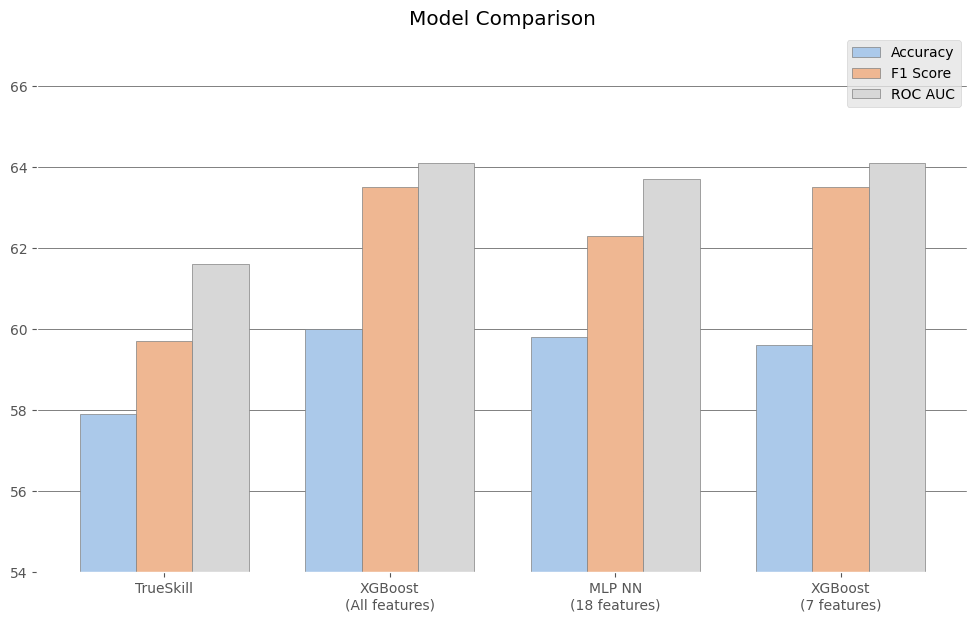
\includegraphics[width=1.1\textwidth]{Figures/results-bars.png}
	\end{adjustbox}
	\caption{Comparison of best accuracy, F1-score, and AUC ROC attained for models trained with different amounts of features}
	\label{fig:full-data-bars}
\end{figure}

\subsection{Filtered datasets}

\subsubsection{Excluding BO1 matches}

A common conception in the Counter-Strike community is that best-of-1 matches are more unpredictable and upsets are more likely. This is a reasonable expectation considering that fewer round wins are required to win the match, which can lead to more volatile outcomes. One would therefore expect an improvement in predictive accuracy when ignoring BO1 matches.

The dataset used for this analysis consisted of 8320 matches in total split using the same 80:20 ratio. 6656 matches were used to train the models, and their performance was evaluated by testing them on 1664 matches. The 18 selected features were determined using the feature importance graphs obtained earlier.

\begin{table}[h!]
	\centering
	\small
	\begin{adjustbox}{center} % Center the table
		\begin{tabular}{ |l|c|c|c|c|c|c| }
			\hline
			\rule{0pt}{2.6ex} \textbf{Model} & \textbf{Train ACC} & \textbf{Test ACC} & \textbf{Precision} & \textbf{Recall} & \textbf{F1 Score} & \textbf{ROC AUC} \\
			\hline
			\rule{0pt}{2.6ex} TrueSkill                 & 58.8 & 59.2 & 59.3 & 62.3 & 60.8 & 63.7 \\ \hline
			\rule{0pt}{2.6ex} Logistic regression       & 61.3 & 61.7 & 60.6 & 69.9 & 64.9 & 65.6 \\
			\rule{0pt}{2.6ex} Random forests            & 65.5 & 61.3 & 60.1 & \textbf{70.6} & 64.9 & 66.0 \\
			\rule{0pt}{2.6ex} Support vector machine    & 61.3 & 61.7 & \textbf{60.8} & 68.8 & 64.6 & 65.5 \\
			\rule{0pt}{2.6ex} XGBoost                   & 63.7 & \textbf{61.9} & \textbf{60.8} & 69.9 & \textbf{65.0} & \textbf{66.3} \\
			\rule{0pt}{2.6ex} Gaussian Naive Bayes      & 60.4 & 59.4 & 58.5 & 68.2 & 63.0 & 63.3 \\
			\rule{0pt}{2.6ex} Multilayer perceptron     & 62.1 & 61.1 & 60.2 & 68.8 & 64.2 & 65.9 \\
			\rule{0pt}{2.6ex} $k$-nearest neighbours 	& 61.2 & 60.9 & 59.9 & 69.2 & 64.2 & 65.7 \\
			\hline
		\end{tabular}
	\end{adjustbox}
	\caption{Performance of ML models trained with all features on dataset which excludes BO1 matches}
	\label{table:3}
\end{table}

The baseline TrueSkill model's classification accuracy improved slightly from 57.9\% to 59.2\%, a modest 1.3\% improvement. Almost all of models achieved over 60\% accuracy. XGBoost once again achieved the best performance, followed by SVM and logistic regression. These results empirically support the notion that Best-of-1's are more difficult to predict.

% Hyperparameters used
% LOG {'C': 1, 'penalty': 'l2', 'solver': 'liblinear'}
% RAN {'criterion': 'gini', 'max_depth': 5, 'max_features': 'log2', 'min_samples_leaf': 4, 'min_samples_split': 4, 'n_estimators': 300}
% SVM {'C': 0.1, 'gamma': 'scale', 'kernel': 'linear'}
% XGB {'learning_rate': 0.025, 'max_depth': 2, 'n_estimators': 200}
% GNV {'var_smoothing' : '1e-09'}
% MLP {'activation': 'tanh', 'alpha': 0.001, 'hidden_layer_sizes': (10,100,10), 'learning_rate_init': 0.001, 'solver': 'sgd'}
% KNN {'n_neighbors': 110, 'p': 1, 'weights': 'uniform'}

\subsubsection{LAN-only}

LAN tournaments are often prestigious events, and it is usually only the top teams who play in these matches. It is thus useful to understand the classification performance for these types of matches. Applying this filter reduces the number of matches significantly. Furthermore, in 2020 and a large part of 2021, almost no LAN matches were played due to the COVID-19 pandemic. The dataset therefore contains only 2130 matches, of which 1704 were used for training and 426 for testing. Note that these include all match formats, including BO1. 

\begin{table}[h!]
	\centering
	\small
	\begin{adjustbox}{center} % Center the table
		\begin{tabular}{ |l|c|c|c|c|c|c| }
			\hline
			\rule{0pt}{2.6ex} \textbf{Model} & \textbf{Train ACC} & \textbf{Test ACC} & \textbf{Precision} & \textbf{Recall} & \textbf{F1 Score} & \textbf{ROC AUC} \\
			\hline
			\rule{0pt}{2.6ex} TrueSkill                 & 54.8 & 59.9 & 59.0 & 64.8 & 61.7 & 62.8 \\ \hline
			\rule{0pt}{2.6ex} Logistic regression       & 58.1 & 60.1 & 59.6 & 62.4 & 61.0 & 63.5 \\
			\rule{0pt}{2.6ex} Random forests            & 63.8 & 62.4 & \textbf{61.4} & 67.1 & 64.1 & 63.9 \\
			\rule{0pt}{2.6ex} Support vector machine    & 58.0 & \textbf{62.7} & 61.1 & \textbf{70.0} & \textbf{65.2} & \textbf{64.2} \\
			\rule{0pt}{2.6ex} XGBoost                   & 67.2 & 60.3 & 59.7 & 63.4 & 61.5 & 61.8 \\
			\rule{0pt}{2.6ex} Gaussian Naive Bayes      & 57.0 & 59.9 & 59.5 & 61.5 & 60.5 & 61.7 \\
			\rule{0pt}{2.6ex} Multilayer perceptron     & 57.3 & 59.2 & 58.3 & 64.3 & 61.2 & 61.1 \\
			\rule{0pt}{2.6ex} $k$-nearest neighbours 	& 59.2 & 58.0 & 56.9 & 65.7 & 61.0 & 62.8 \\
			\hline
		\end{tabular}
	\end{adjustbox}
	\caption{Performance of ML models trained with selected features on dataset with only LAN matches included}
	\label{table:0}
\end{table}

SVM was the surprising winner under these circumstances, with random forests the runner-up. XGBoost and the MLP did not fare as well as before. This was the first time an ML model achieved an accuracy in excess of 62\%. The dataset was, however, far smaller for this filter than with previous testing. That being said, the 2.8\% improvement over the baseline TrueSkill model was more significant than previous deltas. These results empirically support the idea that LAN matches are more predictable than online matches.

% Hyperparameters used
% LOG {'C': 0.01, 'penalty': 'l2', 'solver': 'liblinear'}
% RAN {'criterion': 'gini', 'max_depth': 5, 'max_features': 'log2', 'min_samples_leaf': 4, 'min_samples_split': 4, 'n_estimators': 300}
% SVM {'C': 0.1, 'gamma': 'scale', 'kernel': 'linear'}
% XGB {'learning_rate': 0.025, 'max_depth': 2, 'n_estimators': 200}
% GNV {'var_smoothing' : '1e-09'}
% MLP {'activation': 'relu', 'alpha': 0.001, 'hidden_layer_sizes': (10,100,10), 'learning_rate_init': 0.001, 'solver': 'sgd'}
% KNN {'n_neighbors': 110, 'p': 1, 'weights': 'uniform'}

\subsubsection{Rating cut-off}

As discussed previously, the full dataset includes all matches played where at least one of the team's was ranked in the Top-50 on HLTV's world ranking. Does varying this constraint meaningfully impact the overall predictability of matches? To test this hypothesis, the rank threshold was adjusted to only consider matches played where at least one of the teams were ranked in the Top-30 and Top-15 respectively. The results are tabulated in Tables \ref{table:4} and \ref{table:5} below.

\textbf{Top-30}

This filter removed a sizeable number of matches from the dataset, leaving 7115 for analysis. 5692 were used for training the models and 1423 for testing.


\begin{table}[h!]
	\centering
	\small
	\begin{adjustbox}{center} % Center the table
		\begin{tabular}{ |l|c|c|c|c|c|c| }
			\hline
			\rule{0pt}{2.6ex} \textbf{Model} & \textbf{Train ACC} & \textbf{Test ACC} & \textbf{Precision} & \textbf{Recall} & \textbf{F1 Score} & \textbf{ROC AUC} \\
			\hline
			\rule{0pt}{2.6ex} TrueSkill 				& 57.4 & 58.0 & 57.8 & 62.4 & 60.0 & 61.5 \\ \hline
			\rule{0pt}{2.6ex} Logistic regression 		& 60.4 & 59.3 & 57.6 & 73.7 & \textbf{64.6} & 63.3 \\
			\rule{0pt}{2.6ex} Random forests 			& 62.9 & 58.1 & 56.6 & \textbf{73.0} & 63.7 & 61.7 \\
			\rule{0pt}{2.6ex} Support vector machine 	& 61.3 & 58.6 & 57.7 & 67.0 & 62.0 & 62.8 \\
			\rule{0pt}{2.6ex} XGBoost 					& 62.9 & \textbf{59.5} & 58.0 & 71.6 & 64.1 & \textbf{64.3} \\
			\rule{0pt}{2.6ex} Gaussian Naive Bayes 		& 58.2 & 57.2 & 57.8 & 56.3 & 57.0 & 60.8 \\
			\rule{0pt}{2.6ex} Multilayer perceptron		& 61.7 & 59.0 & \textbf{60.7} & 53.3 & 56.8 & 62.0 \\
			\rule{0pt}{2.6ex} $k$-nearest neighbours 	& 64.7 & 52.8 & 53.0 & 58.4 & 55.5 & 54.2 \\
			\hline
		\end{tabular}
	\end{adjustbox}
	\caption{Performance of ML models trained with selected features on dataset consisting only of Top-30 matches}
	\label{table:4}
\end{table}

The results obtained were very similar to the full dataset, with the baseline benchmark only improving its accuracy by 0.1\%. XGBoost and MLP once again proved to be the strongest models, which was expected given the earlier results. That being said, the best accuracy attained actually decreased slightly, from 59.8\% to 59.5\%.

\textbf{Top-15}

The ranking threshold was tightened to include only matches with at least one Top-15 team. This constrained the dataset to 3756 matches, of which 3004 were used for training and 752 for testing.

\begin{table}[h!]
	\centering
	\small
	\begin{adjustbox}{center} % Center the table
		\begin{tabular}{ |l|c|c|c|c|c|c| }
			\hline
			\rule{0pt}{2.6ex} \textbf{Model} & \textbf{Train ACC} & \textbf{Test ACC} & \textbf{Precision} & \textbf{Recall} & \textbf{F1 Score} & \textbf{ROC AUC} \\
			\hline
			\rule{0pt}{2.6ex} TrueSkill 				& 58.2 & 58.5 & 59.3 & 62.6 & 60.9 & 61.6 \\ \hline
			\rule{0pt}{2.6ex} Logistic regression 		& 62.5 & 57.6 & 56.9 & 73.5 & 64.1 & 62.3 \\
			\rule{0pt}{2.6ex} Random forests			& 61.8 & 58.6 & 57.1 & \textbf{79.9} & \textbf{66.6} & 62.4 \\
			\rule{0pt}{2.6ex} Support vector machine 	& 63.3 & 58.1 & 57.0 & 77.1 & 65.5 & 63.7 \\
			\rule{0pt}{2.6ex} XGBoost 					& 66.5 & \textbf{62.0} & 61.8 & 69.1 & 65.2 & \textbf{65.8} \\
			\rule{0pt}{2.6ex} Gaussian Naive Bayes 		& 59.0 & 58.4 & \textbf{61.9} & 50.3 & 55.5 & 62.1 \\
			\rule{0pt}{2.6ex} Multilayer perceptron     & 64.4 & 60.2 & 59.5 & 71.9 & 65.1 & 61.9 \\
			\rule{0pt}{2.6ex} $k$-nearest neighbours 	& 66.3 & 51.6 & 52.7 & 61.3 & 56.7 & 54.0 \\
			\hline
		\end{tabular}
	\end{adjustbox}
	\caption{Performance of ML models trained with selected features on dataset consisting only of Top-15 matches}
	\label{table:5}
\end{table}

The results here mirror what was found with the LAN-only filter. Indeed, there is significant overlap between these two datasets, as teams which attend LAN events tend to be higher-ranked. XGBoost proved its superior classification ability once more, attaining 62\%. It is noteworthy that each model (except Gaussian Naive Bayes) exhibited significantly better recall than precision. This means that the models tend towards positive classifications: true positives were often identified, however, more false positives also occurred.

The improvement in model performance is likely due to the increased proportion of lopsided matches (Top-15 vs a lower ranked team) present in this subset of the data, which should be easier to predict.

\subsection{Summary}

Machine learning techniques outperform the baseline classification performance, albeit usually only by a few percentage points. XGBoost was found to consistently outperform the other methods employed, achieving 62\% accuracy on the dataset which excluded BO1s. SVM and MLP also delivered good performance, sometimes beating XGBoost. In the LAN-only subset, SVM achieved 62.7\% accuracy.

The results suggest that LAN matches are more predictable than online matches, and that matches involving a higher-ranked team are generally easier to predict than a match with lower ranked teams. Additionally, BO3 and BO5 matches are easier to predict than BO1 matches.

Furthermore, it was found that incorporating many features did not measurably improve the predictive power of the models. Key features could be identified using filter and wrapper techniques, but also from feature importance metrics produced by the models themselves. Training using a smaller subset of only the most relevant features reduced the tendency for models to overfit the training data while simultaneously reducing the computational requirements. These smaller models produced almost identical performance to the fully-featured models. 


\section{Betting odds: generated vs real}

The odds generated by the various models all exhibited a high correlation with the bookmaker odds, as shown in Table \ref{table:bettingperformance}. As explained in \ref{bettingstats}, the correlation, mean absolute error (MAE), and root-mean squared error (RMSE) for each model is reported. These measure the discrepancy between real odds offered by bookmakers and the odds generated by the models. Bet \% refers to the proportion of matches which were deemed to be worth betting on. The P/L column is the total number of betting units won or lost by the end of the betting period.

\begin{table}[h!]
	\centering
	\small
	\begin{adjustbox}{center} % Center the table
		\begin{tabular}{ |l|c|c|c|c|c|c|c| }
			\hline
			\rule{0pt}{2.6ex} \textbf{Model} & \textbf{Correlation} & \textbf{MAE} & \textbf{RMSE} & \textbf{Bet \%} & \textbf{Win \%} & \textbf{Loss \%} & \textbf{P/L} \\
			\hline
			\rule{0pt}{2.6ex} TrueSkill                 & 0.727 & 0.104 & 0.137 & 79.02 & 45.45 & 54.55 & -1.77 \\ \hline
			\rule{0pt}{2.6ex} Logistic regression       & 0.815 & 0.099  & 0.121 & 82.76 & 39.58 & 60.42 & 27.80 \\
			\rule{0pt}{2.6ex} Random forests            & 0.815 & 0.101 & 0.124 & 81.61 & 39.08 & 60.92 & 25.98 \\
			\rule{0pt}{2.6ex} Support vector machine    & 0.803 & 0.100 & 0.123 & 82.47 & 39.02 & 60.98 & 23.72 \\
			\rule{0pt}{2.6ex} XGBoost                   & \textbf{0.855} &  \textbf{0.088} & \textbf{0.108} & 81.90 & 38.60 & 61.40 & 21.38 \\
			\rule{0pt}{2.6ex} Gaussian Naive Bayes      & 0.774 & 0.102 & 0.135 & 80.17 & \textbf{51.25} &\textbf{ 48.75} & 15.27 \\
			\rule{0pt}{2.6ex} Multilayer perceptron     & 0.801 & 0.097  & 0.120 & \textbf{84.20} & 38.23 & 61.77 & 16.70 \\
			\rule{0pt}{2.6ex} $k$-nearest neighbours 	& 0.740 & 0.105 & 0.130 & 81.90 & 40.70 & 59.30 & \textbf{32.78} \\
			\hline
		\end{tabular}
	\end{adjustbox}
	\caption{Comparison of generated odds to real-world betting odds and per-model profit/loss}
	\label{table:bettingperformance}
\end{table}

The betting performance is of particular interest, as every ML model was profitable despite having a low percentage of winning bets relative to their classification accuracy. This counter-intuitive result is explained by the models assigning a higher probability (but still less than 50\%) to the underdog than what was implied by the bookmaker odds. The models effectively preferred to bet on the teams they predicted to lose. The large payouts from winning underdog bets offset the more frequent losses, resulting in an overall profitable strategy.

Every model considered over 80\% of the matches as worth betting on, with bookmakers offering favourable odds; odds for one of the teams being greater than what the model generated. The MLP produced the most avid betting activity, with 84\% of matches being bet on.

XGBoost, the model which repeatedly produced the most accurate classifications, shared the greatest overlap with the real-world odds, with a correlation of 0.855, MAE of 0.088 and RMSE of 0.108.

The most profitable model, $k$-NN, disagreed with the bookmaker odds the most; it had the lowest correlation of 0.740 and highest errors of all the ML models. 

The cumulative profit/loss for $k$-NN is plotted in Figures \ref{fig:profit-match} and \ref{fig:profit-date}. The first shows the profit/loss on a match-by-match basis, where the second shows the profit/loss with the date as the x-axis. The various horizontal lines in Figure \ref{fig:profit-date} are periods in which no matches were bet on. 

\begin{figure}[h]
	\centering
	\begin{adjustbox}{center}
		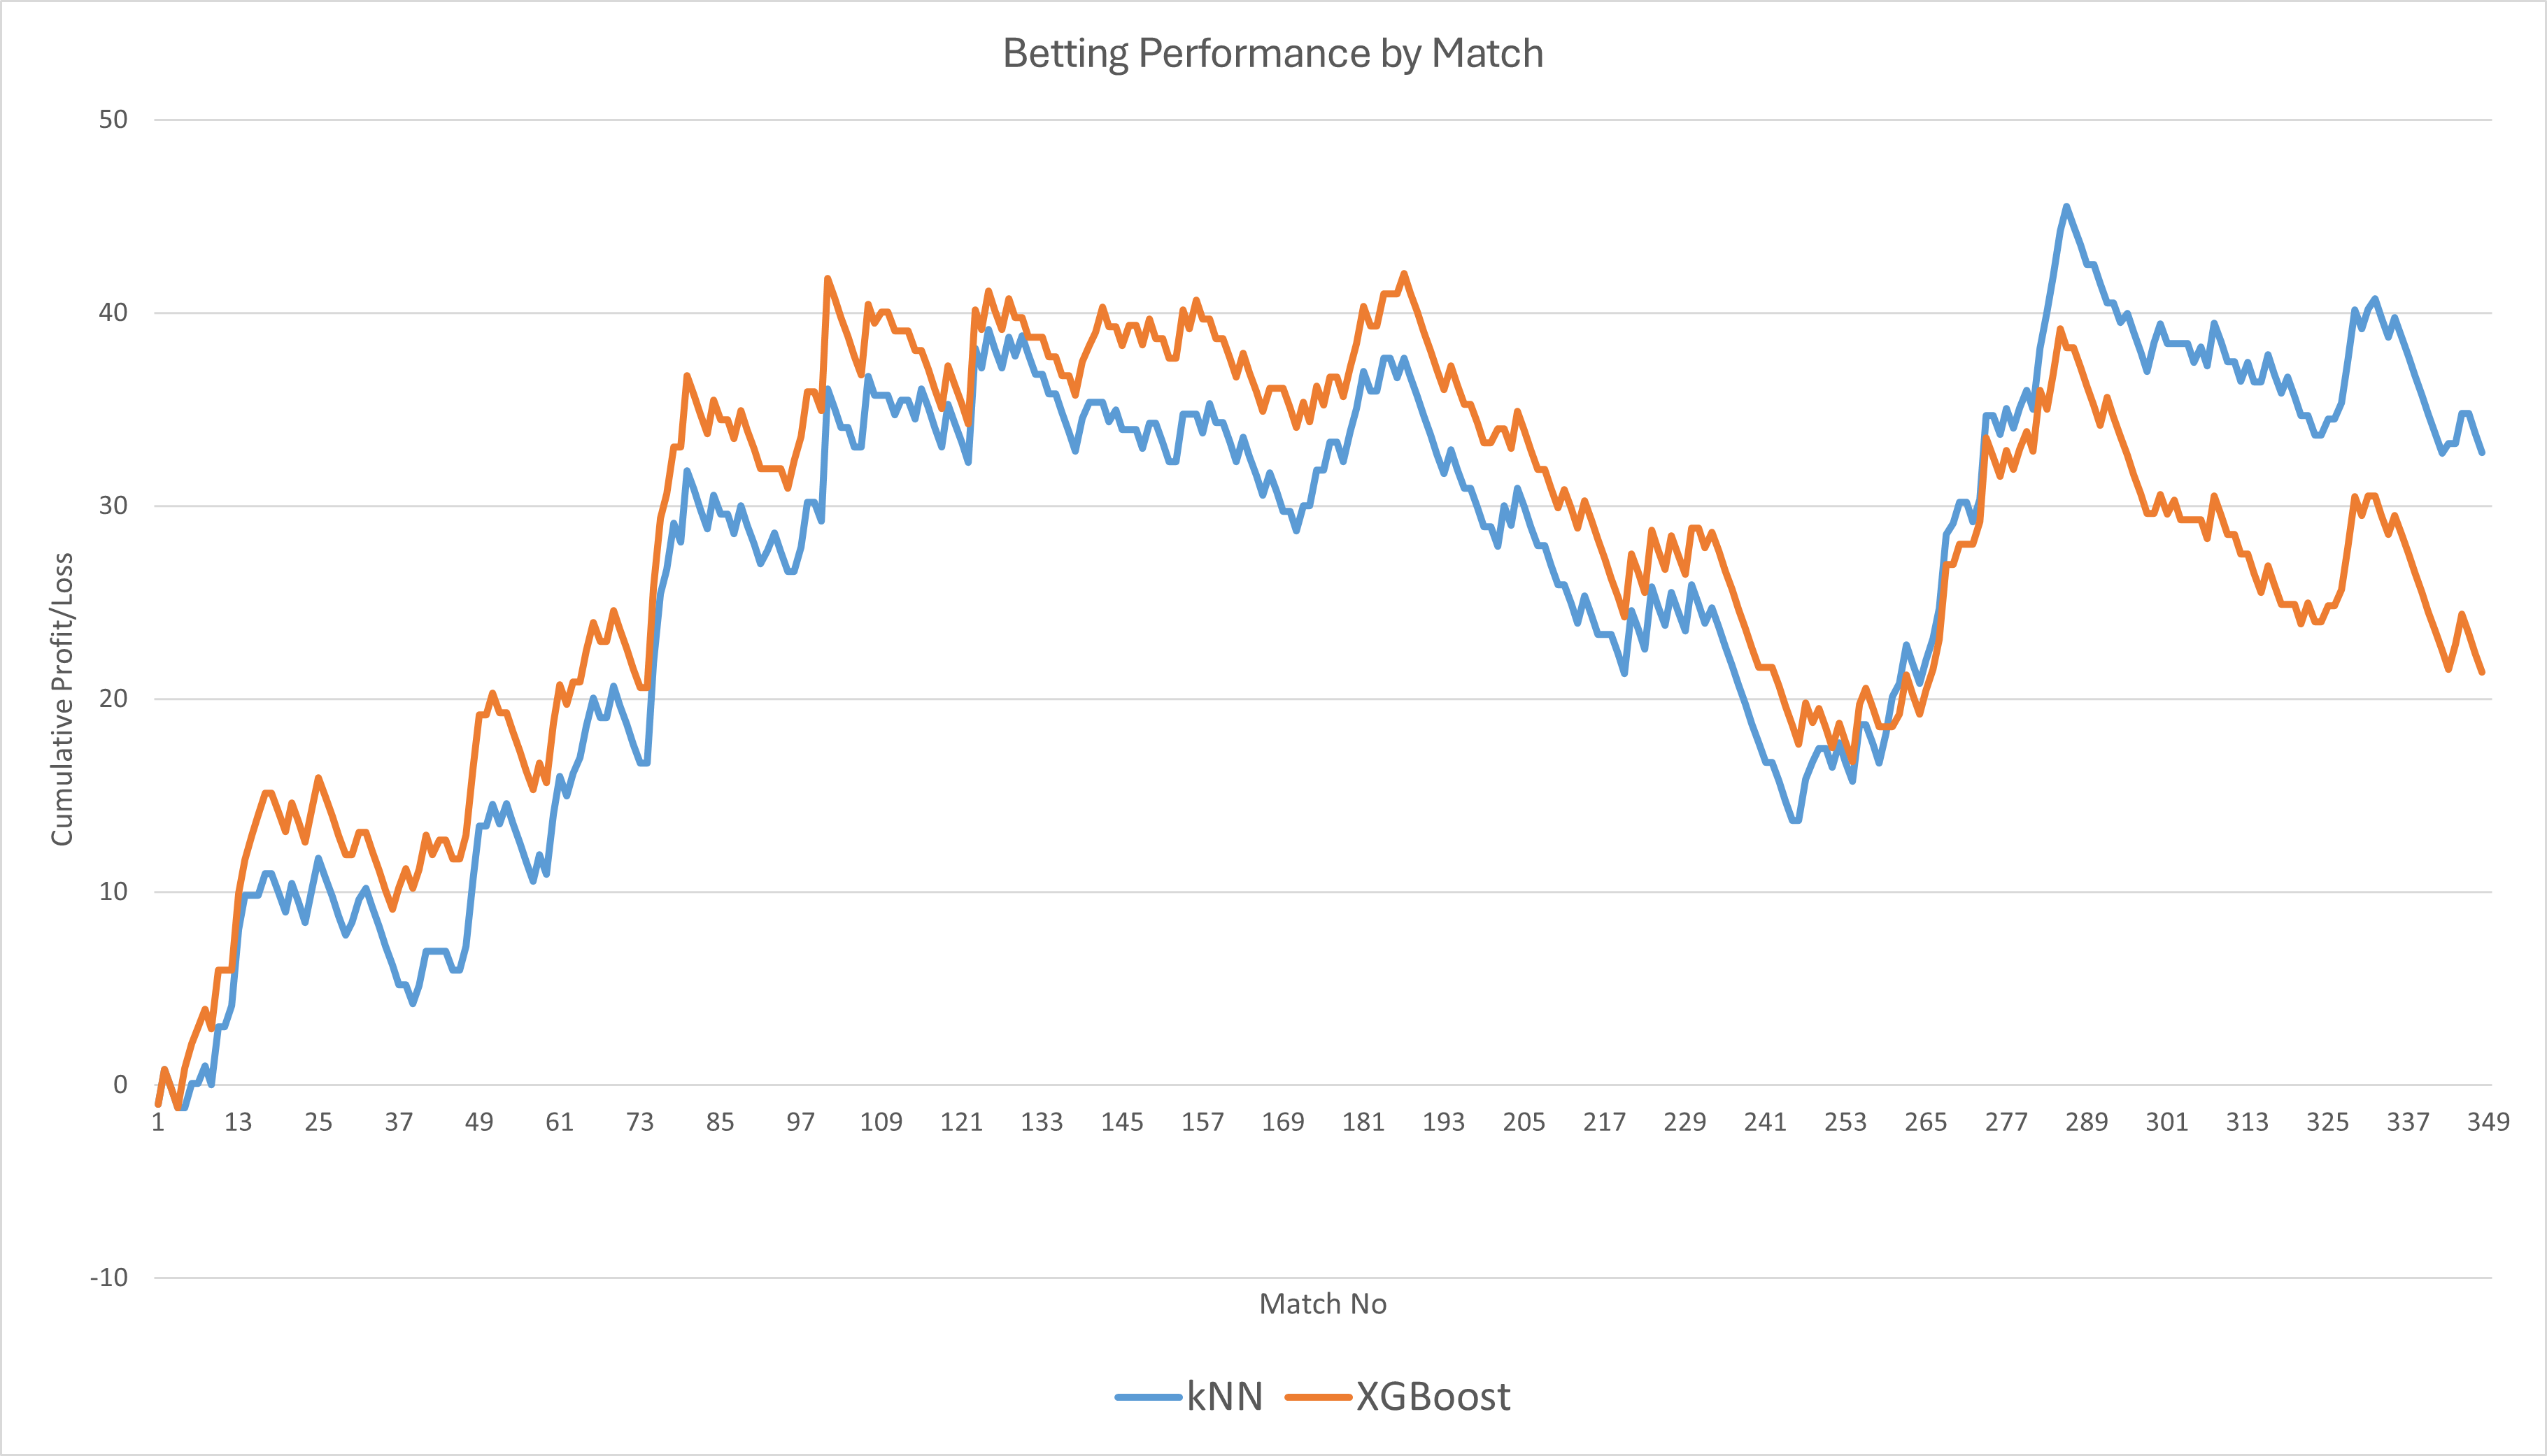
\includegraphics[width=\textwidth]{Figures/profit-match-2.png}
	\end{adjustbox}
	\caption{Cumulative profit/loss for $k$-NN and XGBoost (by match number)}
	\label{fig:profit-match}
\end{figure}

\begin{figure}[h]
	\centering
	\begin{adjustbox}{center}
		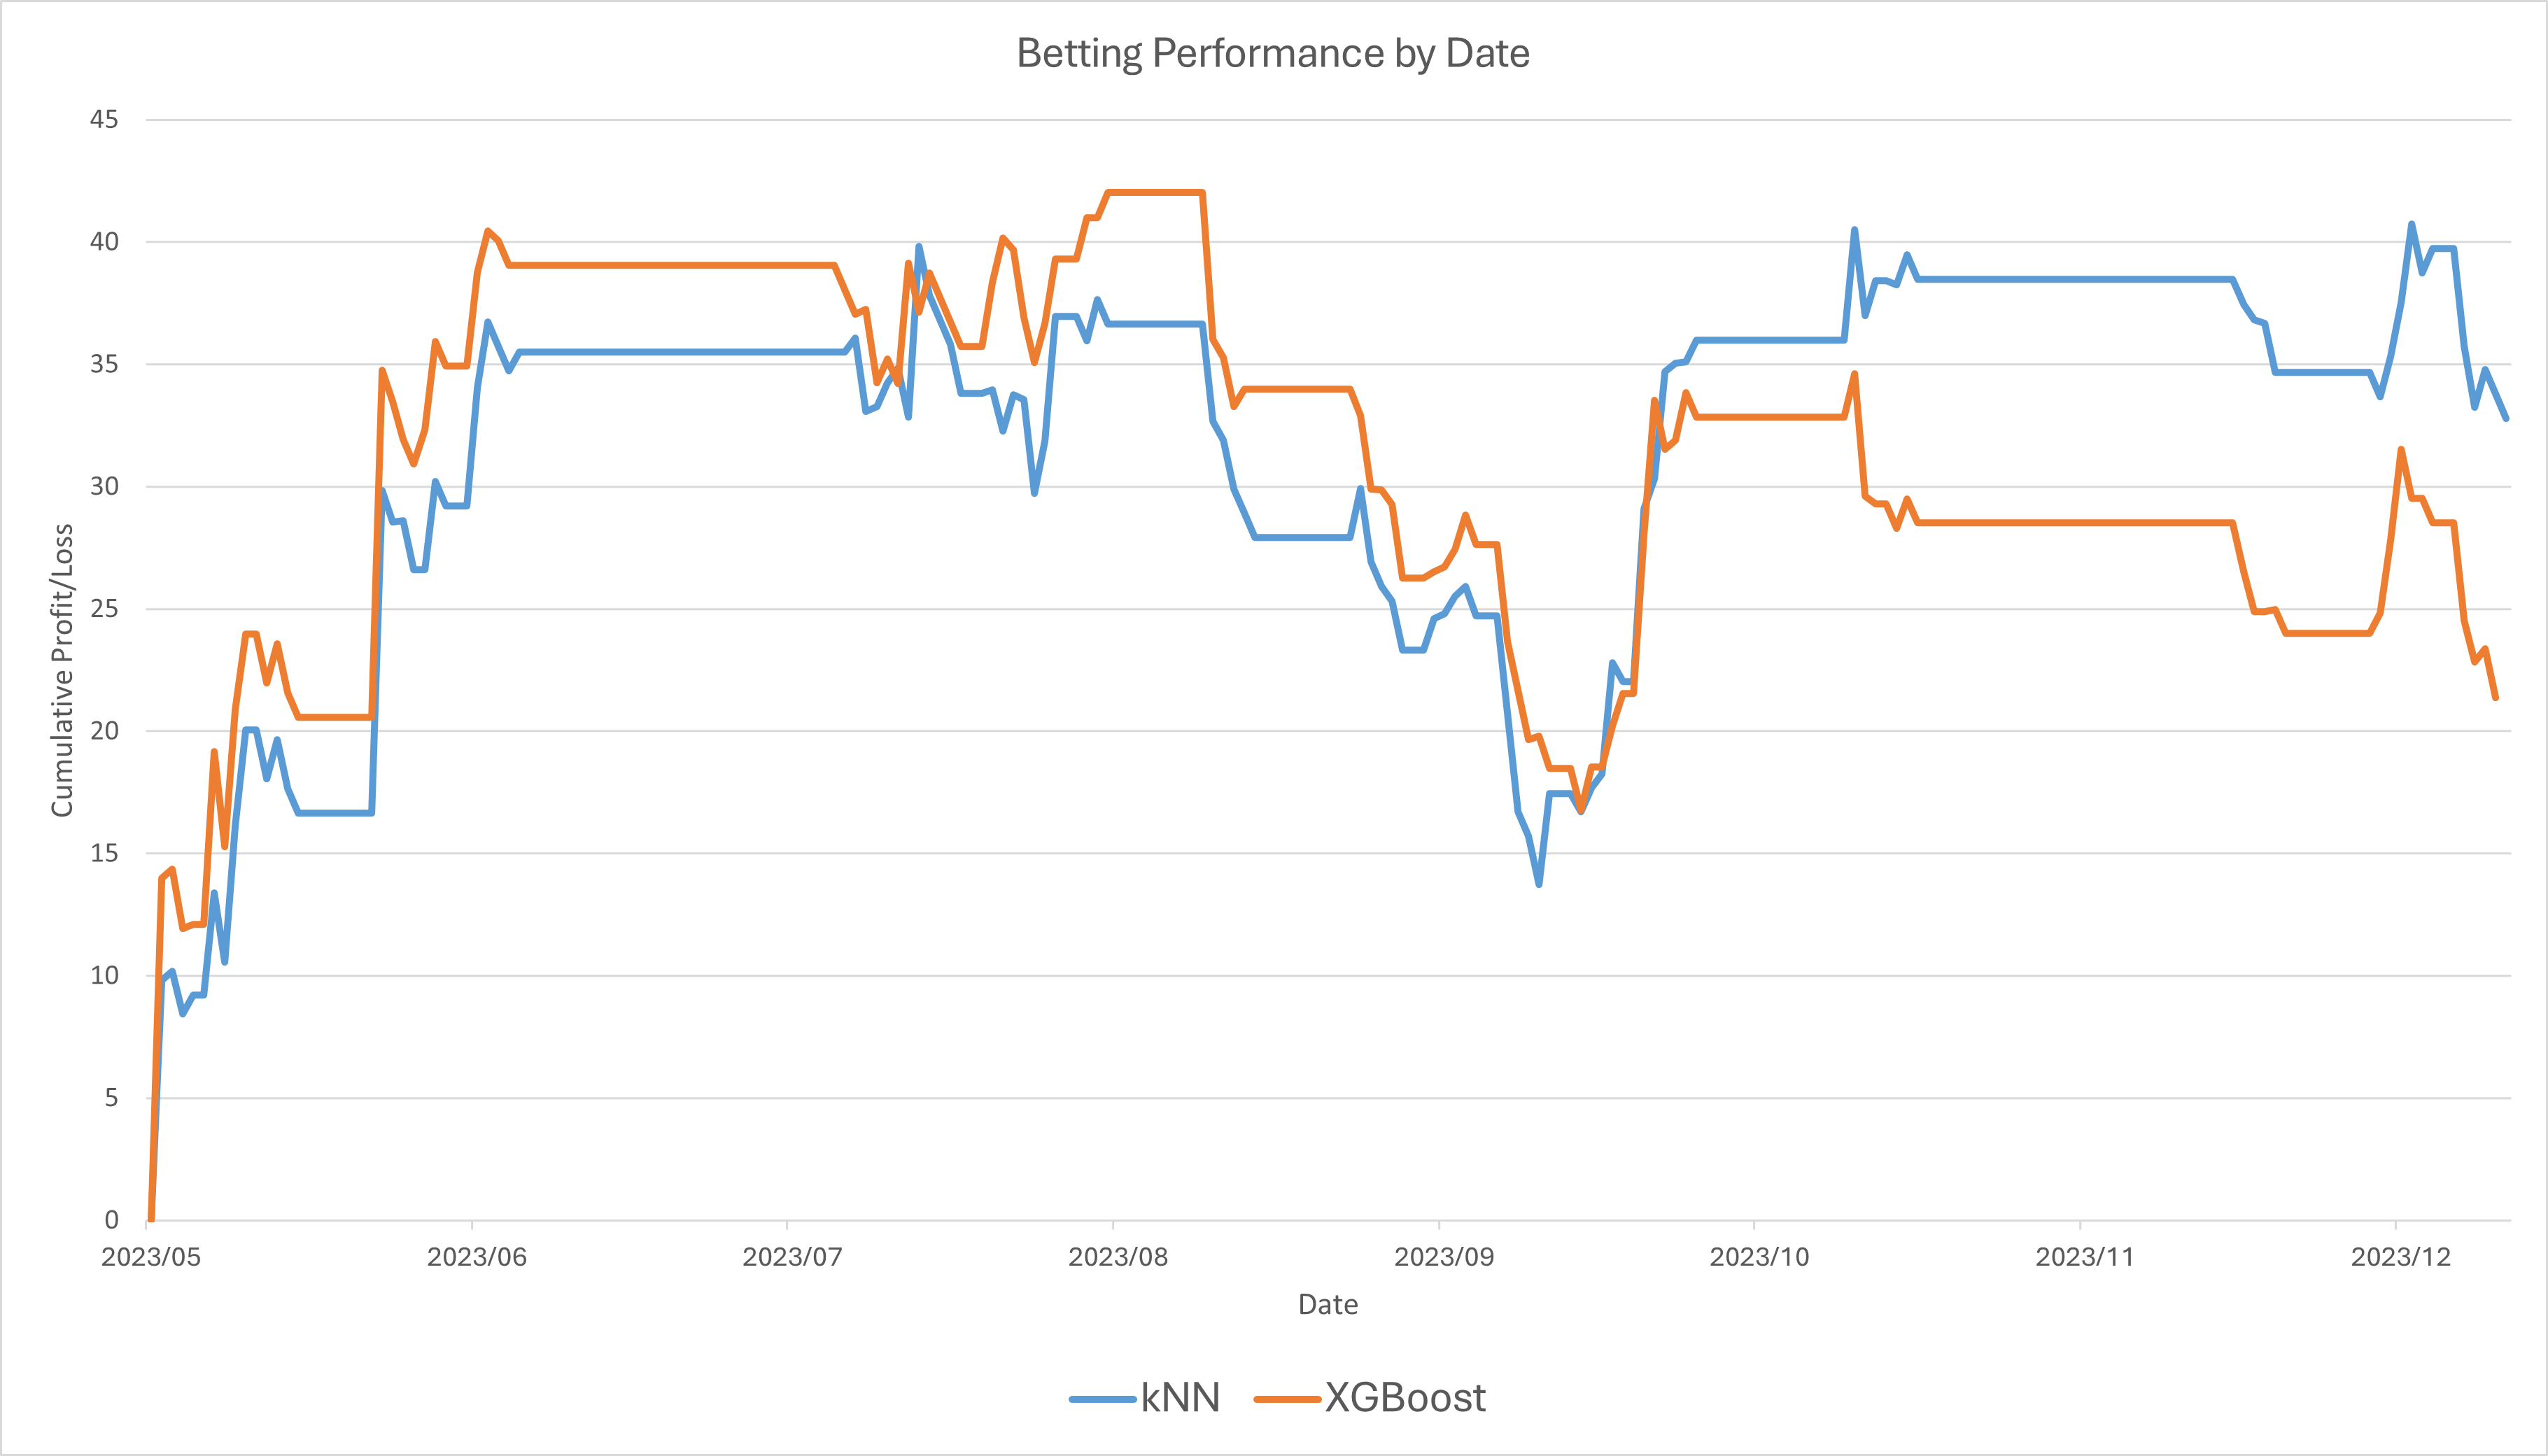
\includegraphics[width=\textwidth]{Figures/profit-date-2.png}
	\end{adjustbox}
	\caption{Cumulative profit/loss for $k$-NN and XGBoost (by date)}
	\label{fig:profit-date}
\end{figure}

It is interesting to note that the model which deviated most from the bookmaker odds was the most profitable. $k$-NN only shared a 74\% correlation with the bookmaker odds. The raw betting data for the $k$-NN model is included in the Appendix. It was found by observation that it would generate very high probabilities (>95\%) for teams more often than the other models, resulting in more "overdog" bets being placed. 

This was in contrast to the other, more accurate models which found most matches to be more balanced. In other words, these models often estimated the underdog as having a higher probability of victory than what the bookmaker odds suggested. They therefore placed underdog bets at a higher rate.

These results suggest that bookmaker odds exhibit some degree of bias which is exploitable. Over a relatively large sample size of matches (n=\matchesBet{}), the machine learning algorithms were all able to make a profit on the esports betting market by considering features generated from historical match data only. Further investigation into optimizing the betting strategy employed may yield even greater profits. 







 
\chapter{Conclusion}
\label{Conclusion}

\section{Key Findings}

Professional Counter-Strike matches are difficult to predict. Incorporating more than a hundred statistics into the prediction process does not measurably improve the predictive power of a model when compared to a model with fewer, more important features. The best accuracy attained for match prediction was 62.7\% when considering only matches played in a LAN environment. For matches played in a BO3 or BO5 maps format, 61.9\% of the match outcomes were correctly predicted. When considering the full dataset of matches played in any format, both online or at LAN, and by at least one Top-50 ranked team, the best accuracy decreased to 59.9\%.

The machine learning models which produced the best results were XGBoost configured to have a large number of estimators with a low maximum tree depth, MLP Neural Networks with a small number of hidden layers and nodes per layer, and Support Vector Machines with a linear kernel. The performance attained by these models were a 2-3\% improvement over the base model, depending on the measure (classification accuracy, $F_1$-score, and AUC ROC).

The baseline model used was a rating system known as TrueSkill, where each player or team's strength is modelled as a Gaussian distribuion. Player TrueSkill ratings are adjusted after every match played. These ratings alone provide good predictions of match outcomes without the need for machine learning techniques, and performed better than both HLTV's world ranking and an Elo rating system. The TrueSkill-related features were consistently ranked as most important by the feature selection techniques employed.

The betting simulation results were surprising. Every model found at least 79\% of the matches were worth betting on. In these cases, the win-probability generated was higher than what the bookmaker odds implied for one of the teams. In these cases, a 1 unit bet was placed on the "undervalued" team. This simple betting strategy proved successful to varying degrees for each of the machine learning models. The best performing model made a profit of 32.78 units over the seven-month betting period, which translates to 0.11 units per match. More advanced betting strategies may be able to leverage the ML-generated predictions to an even greater extent.


\section{Significance of the study}

The key findings of this research bears significance to a number of stakeholders:
\begin{itemize}
	\item Betting Industry\\
	Both \textbf{bookmakers} and \textbf{bettors} can benefit from this research; bookmakers can improve the accuracy of their odd-setting, while bettors can potentially improve their profitability by implementing the insights into their own betting strategies. This research could contribute to bettors making more informed decisions, thereby promoting responsible betting.
	\item Viewer Experience\\\textbf{Commentators} use statistics to support their narratives. \textbf{Broadcasters} can enhance their streams by incorporating data-driven insights, potentially improving viewer engagement. \textbf{Counter-Strike fans} may find entertainment value from a deeper understanding of match predictability.
	\item Tournament Organizers\\
	Predictive information can assist \textbf{tournament organizers} to structure their tournaments and schedules in order to maximize the competitive fairness of their tournaments. They could also be used to design fair qualification systems or choose which teams to invite.
	\item Academia\\
	This research contributes to the understanding of esports betting and predictive modelling of professional Counter-Strike. \textbf{Future researchers} may find it to be a valuable resource for further study into these topics.
	\item Esports Community\\
	Professional teams (\textbf{players}, \textbf{coaches}, and \textbf{analysts}) may find the outputs from the statistical modelling valuable.
	
\end{itemize}

\section{Limitations}

Odds compilation is a private industry. The exact mechanisms used by bookmakers to price odds are not publicised. This makes it difficult to ascertain the extent to which statistical models influence the odds. Other factors, such as bookmaker risk management strategies and user betting behaviour, may also be used to generate the odds.

The data used to train the models was limited to match information and statistics. External factors such as player injuries, team morale, or technical issues were therefore unaccounted for. There is inherent unpredictability to any sport; the accuracy of predictive models are thus subject to the quality of the available data and the modelling techniques employed.

The feature engineering, although extensive, was not comprehensive. The historical features were generated using a three-month sliding window of a team's past performance. For newly formed line-ups, this data is not as informative as established teams. This could have been mitigated by considering a team "core" consisting of 3 or 4 players. Furthermore, 3 months may be too large or too small a window; varying this time-window was not explored. Incorporating features that more accurately describe the trends in a team's performance may lead to stronger predictions. An example of this was the 'winning streak' feature. Additional feature selection methods, as well as dimensionality reduction techniques, could have also been explored.

The list of machine learning techniques implemented was not exhaustive. For example, a recurrent neural network such as long short-term memory (LSTM) may be more appropriate for chronological data. Additionally, an ensemble model taking into account the outputs of multiple models may achieve better results than any individual model. These hypotheses were not tested.

The data segmentation method employed does not accurately reflect a real-world scenario, where all known match data would be used to train the model and the test would be a future fixture. An approach which better resembles real-world use would be to incrementally increase the training dataset, each time using all of the data for training, leaving only 1 match for testing. In the next iteration, this match would be added to the training set and the next match becomes the test set. This approach would be more repesentative of a real-world model, however at the cost of being significantly more computationally expensive.

Finally, for testing each model's betting performance, the betting strategy used was fairly basic. More complex strategies could have been explored, such as the use of a dynamic wager which depends on the odds differential, or perhaps combining the predictions from different models. The number of matches tested was also a fairly low amount (\matchesBet{}) - more odds data could have been collected and tested.

\section{Future work}

Given the limitations described, future work could expand on the findings made here in a number of ways:

\begin{enumerate}
	\item An investigation of how external factors, such as player injuries, team morale, and even social media sentiments, can influence match prediction
	\item There is room for more sophisticated feature engineering techniques. As mentioned above, adjusting the sliding window of data to find the optimal period to balance recency and relevance, as well as including features that describe the team's performance trajectory or trends.
	\item Investigating more advanced machine learning techniques, such as LSTMs, ensemble methods, or even transformer models. These techniques may be able to outperform the models used in this research.
	\item Application of an iterative data segmentation method, which more closely mirrors how a model would be used in real-world applications.
	\item Collaboration with bookmakers and odds compilers to understand the methods employed in the betting industry. This may help to foster transparency and innovation in the field.
	\item The development and testing of more complex betting strategies on a larger dataset of matches would make the findings more robust.
\end{enumerate}

%----------------------------------------------------------------------------------------
%	THESIS CONTENT - APPENDICES
%----------------------------------------------------------------------------------------

\appendix % Cue to tell LaTeX that the following "chapters" are Appendices

% Include the appendices of the thesis as separate files from the Appendices folder
% Uncomment the lines as you write the Appendices

% Appendix A

\chapter{Raw betting data} % Main appendix title

\label{dix:betting-data} % For referencing this appendix elsewhere, use \ref{AppendixA}

The generated odds used in this table were generated using the $k$-nearest neighbours algorithm.

% Please add the following required packages to your document preamble:
% \usepackage{longtable}
% Note: It may be necessary to compile the document several times to get a multi-page table to line up properly
\begin{small}
% Please add the following required packages to your document preamble:
% \usepackage{longtable}
% Note: It may be necessary to compile the document several times to get a multi-page table to line up properly
\begin{longtable}{|l|l|l|l|l|l|l|l|}
	\hline
	\multicolumn{1}{|c|}{\textbf{Date}} & \multicolumn{1}{c|}{\textbf{Match}} & \multicolumn{1}{c|}{\textbf{Book Odds}} & \multicolumn{1}{c|}{\textbf{Gen. Odds}} & \multicolumn{1}{c|}{\textbf{Bet}} & \multicolumn{1}{c|}{\textbf{W/L}} & \multicolumn{1}{c|}{\textbf{Amount}} & \multicolumn{1}{c|}{\textbf{P/L}} \\ \hline
	\endhead
	%
	05/08                               & monte : faze                        & 2.68 : 1.44                             & 1.96 : 2.04                             & monte                             & L                                 & -1                                   & -1                                \\ \hline
	05/08                               & pain : fluxo                        & 1.43 : 2.80                             & 1.80 : 2.24                             & fluxo                             & W                                 & 1.8                                  & 0.8                               \\ \hline
	05/08                               & g2 : mongolz                        & 1.10 : 6.44                             & 1.53 : 2.89                             & mongolz                           & L                                 & -1                                   & -0.2                              \\ \hline
	05/08                               & gamerl : col                        & 1.75 : 2.06                             & 1.43 : 3.33                             & gamerl                            & L                                 & -1                                   & -1.2                              \\ \hline
	05/08                               & forze : grayhound                   & 1.35 : 3.07                             & 1.41 : 3.44                             &                                   &                                   & 0                                    & -1.2                              \\ \hline
	05/08                               & apeks : liquid                      & 2.27 : 1.60                             & 2.16 : 1.86                             & apeks                             & W                                 & 1.27                                 & 0.07                              \\ \hline
	05/08                               & nip : mouz                          & 1.90 : 1.85                             & 2.16 : 1.86                             &                                   &                                   & 0                                    & 0.07                              \\ \hline
	05/08                               & og : ence                           & 1.93 : 1.82                             & 1.93 : 2.08                             & og                                & W                                 & 0.93                                 & 1                                 \\ \hline
	05/08                               & faze : pain                         & 1.34 : 3.16                             & 1.55 : 2.82                             & pain                              & L                                 & -1                                   & 0                                 \\ \hline
	05/08                               & col : g2                            & 4.03 : 1.22                             & 2.75 : 1.57                             & col                               & W                                 & 3.03                                 & 3.03                              \\ \hline
	05/08                               & apeks : grayhound                   & 1.38 : 2.94                             & 1.47 : 3.14                             &                                   &                                   & 0                                    & 3.03                              \\ \hline
	05/08                               & ence : nip                          & 1.75 : 2.07                             & 2.04 : 1.96                             & nip                               & W                                 & 1.07                                 & 4.1                               \\ \hline
	05/08                               & fluxo : monte                       & 4.97 : 1.17                             & 2.97 : 1.51                             & fluxo                             & W                                 & 3.97                                 & 8.07                              \\ \hline
	05/08                               & gamerl : mongolz                    & 1.42 : 2.75                             & 1.64 : 2.56                             & mongolz                           & W                                 & 1.75                                 & 9.82                              \\ \hline
	05/08                               & forze : liquid                      & 2.27 : 1.59                             & 2.29 : 1.77                             &                                   &                                   & 0                                    & 9.82                              \\ \hline
	05/08                               & mouz : og                           & 1.73 : 2.05                             & 1.77 : 2.29                             &                                   &                                   & 0                                    & 9.82                              \\ \hline
	05/09                               & col : pain                          & 2.14 : 1.68                             & 1.83 : 2.20                             & col                               & W                                 & 1.14                                 & 10.96                             \\ \hline
	05/09                               & grayhound : mongolz                 & 1.91 : 1.85                             & 2.00 : 2.00                             &                                   &                                   & 0                                    & 10.96                             \\ \hline
	05/09                               & forze : monte                       & 2.35 : 1.56                             & 2.12 : 1.90                             & forze                             & L                                 & -1                                   & 9.96                              \\ \hline
	05/09                               & nip : og                            & 1.75 : 2.01                             & 2.34 : 1.75                             & og                                & L                                 & -1                                   & 8.96                              \\ \hline
	05/09                               & ence : faze                         & 2.47 : 1.52                             & 2.00 : 2.00                             & ence                              & W                                 & 1.47                                 & 10.43                             \\ \hline
	05/09                               & apeks : g2                          & 3.83 : 1.24                             & 2.08 : 1.93                             & apeks                             & L                                 & -1                                   & 9.43                              \\ \hline
	05/09                               & fluxo : liquid                      & 5.85 : 1.12                             & 2.82 : 1.55                             & fluxo                             & L                                 & -1                                   & 8.43                              \\ \hline
	05/09                               & gamerl : mouz                       & 2.75 : 1.43                             & 2.20 : 1.83                             & gamerl                            & W                                 & 1.75                                 & 10.18                             \\ \hline
	05/10                               & gamerl : og                         & 2.57 : 1.49                             & 2.24 : 1.80                             & gamerl                            & W                                 & 1.57                                 & 11.75                             \\ \hline
	05/10                               & mongolz : monte                     & 4.55 : 1.18                             & 2.34 : 1.75                             & mongolz                           & L                                 & -1                                   & 10.75                             \\ \hline
	05/10                               & col : liquid                        & 2.74 : 1.42                             & 2.12 : 1.90                             & col                               & L                                 & -1                                   & 9.75                              \\ \hline
	05/10                               & faze : forze                        & 1.39 : 3.04                             & 1.69 : 2.44                             & forze                             & L                                 & -1                                   & 8.75                              \\ \hline
	05/10                               & grayhound : nip                     & 4.47 : 1.17                             & 2.34 : 1.75                             & grayhound                         & L                                 & -1                                   & 7.75                              \\ \hline
	05/10                               & apeks : pain                        & 1.68 : 2.12                             & 1.64 : 2.56                             & apeks                             & W                                 & 0.68                                 & 8.43                              \\ \hline
	05/11                               & forze : gamerl                      & 1.65 : 2.18                             & 2.04 : 1.96                             & gamerl                            & W                                 & 1.18                                 & 9.61                              \\ \hline
	05/11                               & monte : pain                        & 1.59 : 2.33                             & 1.57 : 2.75                             & monte                             & W                                 & 0.59                                 & 10.2                              \\ \hline
	05/11                               & grayhound : liquid                  & 4.78 : 1.17                             & 2.75 : 1.57                             & grayhound                         & L                                 & -1                                   & 9.2                               \\ \hline
	05/13                               & navi : gamerl                       & 1.32 : 3.29                             & 1.51 : 2.97                             & gamerl                            & L                                 & -1                                   & 8.2                               \\ \hline
	05/13                               & 9ine : liquid                       & 1.83 : 1.92                             & 2.44 : 1.69                             & liquid                            & L                                 & -1                                   & 7.2                               \\ \hline
	05/13                               & furia : monte                       & 1.66 : 2.15                             & 2.12 : 1.90                             & monte                             & L                                 & -1                                   & 6.2                               \\ \hline
	05/13                               & fnatic : nip                        & 2.13 : 1.67                             & 2.50 : 1.67                             & nip                               & L                                 & -1                                   & 5.2                               \\ \hline
	05/13                               & heroic : faze                       & 1.78 : 1.97                             & 1.83 : 2.20                             &                                   &                                   & 0                                    & 5.2                               \\ \hline
	05/13                               & itb : apeks                         & 2.45 : 1.52                             & 2.16 : 1.86                             & itb                               & L                                 & -1                                   & 4.2                               \\ \hline
	05/13                               & vitality : g2                       & 1.96 : 1.79                             & 1.93 : 2.08                             & vitality                          & W                                 & 0.96                                 & 5.16                              \\ \hline
	05/13                               & bne : ence                          & 2.78 : 1.42                             & 1.86 : 2.16                             & bne                               & W                                 & 1.78                                 & 6.94                              \\ \hline
	05/13                               & liquid : navi                       & 2.56 : 1.46                             & 2.68 : 1.59                             &                                   &                                   & 0                                    & 6.94                              \\ \hline
	05/13                               & fnatic : monte                      & 2.00 : 1.76                             & 2.24 : 1.80                             &                                   &                                   & 0                                    & 6.94                              \\ \hline
	05/13                               & vitality : ence                     & 1.54 : 2.39                             & 1.62 : 2.62                             &                                   &                                   & 0                                    & 6.94                              \\ \hline
	05/13                               & heroic : apeks                      & 1.34 : 3.13                             & 1.53 : 2.89                             & apeks                             & L                                 & -1                                   & 5.94                              \\ \hline
	05/13                               & furia : nip                         & 1.79 : 1.97                             & 1.93 : 2.08                             &                                   &                                   & 0                                    & 5.94                              \\ \hline
	05/13                               & 9ine : gamerl                       & 1.62 : 2.23                             & 2.12 : 1.90                             & gamerl                            & W                                 & 1.23                                 & 7.17                              \\ \hline
	05/13                               & bne : g2                            & 4.44 : 1.19                             & 2.04 : 1.96                             & bne                               & W                                 & 3.44                                 & 10.61                             \\ \hline
	05/13                               & faze : itb                          & 1.25 : 3.79                             & 1.75 : 2.34                             & itb                               & W                                 & 2.79                                 & 13.4                              \\ \hline
	05/14                               & navi : nip                          & 1.51 : 2.49                             & 1.59 : 2.68                             &                                   &                                   & 0                                    & 13.4                              \\ \hline
	05/14                               & fnatic : gamerl                     & 1.68 : 2.13                             & 2.34 : 1.75                             & gamerl                            & W                                 & 1.13                                 & 14.53                             \\ \hline
	05/14                               & ence : itb                          & 1.30 : 3.36                             & 1.64 : 2.56                             & itb                               & L                                 & -1                                   & 13.53                             \\ \hline
	05/14                               & apeks : bne                         & 1.74 : 2.03                             & 2.00 : 2.00                             & bne                               & W                                 & 1.03                                 & 14.56                             \\ \hline
	05/14                               & heroic : liquid                     & 1.39 : 2.87                             & 1.90 : 2.12                             & liquid                            & L                                 & -1                                   & 13.56                             \\ \hline
	05/14                               & monte : vitality                    & 3.21 : 1.33                             & 2.20 : 1.83                             & monte                             & L                                 & -1                                   & 12.56                             \\ \hline
	05/14                               & furia : g2                          & 3.31 : 1.33                             & 1.83 : 2.20                             & furia                             & L                                 & -1                                   & 11.56                             \\ \hline
	05/14                               & 9ine : faze                         & 2.99 : 1.37                             & 2.12 : 1.90                             & 9ine                              & L                                 & -1                                   & 10.56                             \\ \hline
	05/15                               & ence : nip                          & 1.55 : 2.37                             & 1.96 : 2.04                             & nip                               & W                                 & 1.37                                 & 11.93                             \\ \hline
	05/15                               & faze : bne                          & 1.24 : 3.87                             & 1.90 : 2.12                             & bne                               & L                                 & -1                                   & 10.93                             \\ \hline
	05/15                               & fnatic : g2                         & 4.10 : 1.22                             & 2.34 : 1.75                             & fnatic                            & W                                 & 3.1                                  & 14.03                             \\ \hline
	05/15                               & monte : navi                        & 2.96 : 1.38                             & 1.86 : 2.16                             & monte                             & W                                 & 1.96                                 & 15.99                             \\ \hline
	05/15                               & liquid : itb                        & 1.31 : 3.29                             & 1.62 : 2.62                             & itb                               & L                                 & -1                                   & 14.99                             \\ \hline
	05/15                               & apeks : gamerl                      & 1.66 : 2.16                             & 1.86 : 2.16                             & gamerl                            & W                                 & 1.16                                 & 16.15                             \\ \hline
	05/16                               & faze : navi                         & 1.81 : 1.94                             & 1.67 : 2.50                             & faze                              & W                                 & 0.81                                 & 16.96                             \\ \hline
	05/16                               & fnatic : itb                        & 1.45 : 2.64                             & 1.72 : 2.39                             & itb                               & W                                 & 1.64                                 & 18.6                              \\ \hline
	05/16                               & apeks : nip                         & 2.45 : 1.52                             & 2.12 : 1.90                             & apeks                             & W                                 & 1.45                                 & 20.05                             \\ \hline
	05/18                               & heroic : faze                       & 1.61 : 2.24                             & 1.90 : 2.12                             & faze                              & L                                 & -1                                   & 19.05                             \\ \hline
	05/19                               & monte : gamerl                      & 1.53 : 2.42                             & 1.69 : 2.44                             &                                   &                                   & 0                                    & 19.05                             \\ \hline
	05/19                               & liquid : apeks                      & 1.48 : 2.61                             & 1.80 : 2.24                             & apeks                             & W                                 & 1.61                                 & 20.66                             \\ \hline
	05/18                               & vitality : itb                      & 1.12 : 5.85                             & 1.55 : 2.82                             & itb                               & L                                 & -1                                   & 19.66                             \\ \hline
	05/20                               & heroic : gamerl                     & 3.76 : 1.25                             & 1.69 : 2.44                             & heroic                            & L                                 & -1                                   & 18.66                             \\ \hline
	05/20                               & vitality : apeks                    & 1.23 : 3.96                             & 1.62 : 2.62                             & apeks                             & L                                 & -1                                   & 17.66                             \\ \hline
	05/21                               & gamerl : vitality                   & 3.30 : 1.33                             & 2.29 : 1.77                             & gamerl                            & L                                 & -1                                   & 16.66                             \\ \hline
	05/29                               & furia : og                          & 1.75 : 2.01                             & 1.77 : 2.29                             &                                   &                                   & 0                                    & 16.66                             \\ \hline
	05/29                               & g2 : nouns                          & 1.11 : 6.18                             & 1.64 : 2.56                             & nouns                             & W                                 & 5.18                                 & 21.84                             \\ \hline
	05/29                               & heroic : 9z                         & 1.17 : 4.61                             & 1.67 : 2.50                             & 9z                                & W                                 & 3.61                                 & 25.45                             \\ \hline
	05/29                               & fnatic : mouz                       & 2.25 : 1.61                             & 2.16 : 1.86                             & fnatic                            & W                                 & 1.25                                 & 26.7                              \\ \hline
	05/29                               & ence : col                          & 1.29 : 3.42                             & 1.62 : 2.62                             & col                               & W                                 & 2.42                                 & 29.12                             \\ \hline
	05/29                               & liquid : astralis                   & 1.87 : 1.87                             & 1.86 : 2.16                             & liquid                            & L                                 & -1                                   & 28.12                             \\ \hline
	05/29                               & cloud9 : grayhound                  & 1.17 : 4.71                             & 1.59 : 2.68                             & grayhound                         & W                                 & 3.71                                 & 31.83                             \\ \hline
	05/29                               & g2 : og                             & 1.26 : 3.74                             & 1.59 : 2.68                             & og                                & L                                 & -1                                   & 30.83                             \\ \hline
	05/29                               & furia : nouns                       & 1.16 : 5.10                             & 1.64 : 2.56                             & nouns                             & L                                 & -1                                   & 29.83                             \\ \hline
	05/30                               & mouz : heroic                       & 3.15 : 1.34                             & 2.24 : 1.80                             & mouz                              & L                                 & -1                                   & 28.83                             \\ \hline
	05/30                               & fnatic : 9z                         & 1.45 : 2.73                             & 2.04 : 1.96                             & 9z                                & W                                 & 1.73                                 & 30.56                             \\ \hline
	05/30                               & liquid : grayhound                  & 1.12 : 5.81                             & 1.55 : 2.82                             & grayhound                         & L                                 & -1                                   & 29.56                             \\ \hline
	05/30                               & faze : ence                         & 1.66 : 2.16                             & 1.77 : 2.29                             &                                   &                                   & 0                                    & 29.56                             \\ \hline
	05/31                               & og : 9z                             & 1.44 : 2.68                             & 2.04 : 1.96                             & 9z                                & L                                 & -1                                   & 28.56                             \\ \hline
	05/31                               & cloud9 : astralis                   & 1.52 : 2.45                             & 1.83 : 2.20                             & astralis                          & W                                 & 1.45                                 & 30.01                             \\ \hline
	05/30                               & furia : mouz                        & 1.87 : 1.87                             & 1.83 : 2.20                             & furia                             & L                                 & -1                                   & 29.01                             \\ \hline
	05/31                               & col : cloud9                        & 5.35 : 1.14                             & 2.56 : 1.64                             & col                               & L                                 & -1                                   & 28.01                             \\ \hline
	05/31                               & faze : liquid                       & 1.60 : 2.27                             & 1.96 : 2.04                             & liquid                            & L                                 & -1                                   & 27.01                             \\ \hline
	05/31                               & mouz : og                           & 1.69 : 2.12                             & 1.67 : 2.50                             & mouz                              & W                                 & 0.69                                 & 27.7                              \\ \hline
	05/31                               & g2 : heroic                         & 1.84 : 1.91                             & 2.24 : 1.80                             & heroic                            & W                                 & 0.91                                 & 28.61                             \\ \hline
	06/01                               & ence : astralis                     & 2.01 : 1.76                             & 2.39 : 1.72                             & astralis                          & L                                 & -1                                   & 27.61                             \\ \hline
	06/01                               & faze : cloud9                       & 1.75 : 2.03                             & 2.04 : 1.96                             & cloud9                            & L                                 & -1                                   & 26.61                             \\ \hline
	06/02                               & astralis : mouz                     & 1.54 : 2.40                             & 1.62 : 2.62                             &                                   &                                   & 0                                    & 26.61                             \\ \hline
	06/03                               & g2 : faze                           & 1.64 : 2.25                             & 2.29 : 1.77                             & faze                              & W                                 & 1.25                                 & 27.86                             \\ \hline
	06/03                               & heroic : mouz                       & 1.31 : 3.34                             & 1.64 : 2.56                             & mouz                              & W                                 & 2.34                                 & 30.2                              \\ \hline
	06/03                               & ence : faze                         & 2.21 : 1.65                             & 2.29 : 1.77                             &                                   &                                   & 0                                    & 30.2                              \\ \hline
	06/04                               & mouz : ence                         & 2.12 : 1.68                             & 1.83 : 2.20                             & mouz                              & L                                 & -1                                   & 29.2                              \\ \hline
	06/07                               & vitality : imperial                 & 1.08 : 7.85                             & 1.47 : 3.14                             & imperial                          & W                                 & 6.85                                 & 36.05                             \\ \hline
	06/07                               & g2 : cloud9                         & 1.60 : 2.26                             & 2.34 : 1.75                             & cloud9                            & L                                 & -1                                   & 35.05                             \\ \hline
	06/07                               & heroic : col                        & 1.10 : 6.51                             & 1.47 : 3.14                             & col                               & L                                 & -1                                   & 34.05                             \\ \hline
	06/07                               & faze : astralis                     & 1.63 : 2.29                             & 1.75 : 2.34                             &                                   &                                   & 0                                    & 34.05                             \\ \hline
	06/08                               & imperial : g2                       & 4.90 : 1.16                             & 2.50 : 1.67                             & imperial                          & L                                 & -1                                   & 33.05                             \\ \hline
	06/08                               & vitality : cloud9                   & 1.54 : 2.39                             & 1.69 : 2.44                             &                                   &                                   & 0                                    & 33.05                             \\ \hline
	06/08                               & col : astralis                      & 4.68 : 1.19                             & 2.34 : 1.75                             & col                               & W                                 & 3.68                                 & 36.73                             \\ \hline
	06/09                               & heroic : faze                       & 1.70 : 2.12                             & 1.90 : 2.12                             & faze                              & L                                 & -1                                   & 35.73                             \\ \hline
	06/09                               & imperial : col                      & 1.61 : 2.24                             & 1.62 : 2.62                             &                                   &                                   & 0                                    & 35.73                             \\ \hline
	06/09                               & vitality : faze                     & 1.70 : 2.13                             & 1.72 : 2.39                             &                                   &                                   & 0                                    & 35.73                             \\ \hline
	06/10                               & heroic : imperial                   & 1.19 : 4.47                             & 1.55 : 2.82                             & imperial                          & L                                 & -1                                   & 34.73                             \\ \hline
	06/11                               & g2 : vitality                       & 2.01 : 1.76                             & 2.75 : 1.57                             & vitality                          & W                                 & 0.76                                 & 35.49                             \\ \hline
	06/11                               & heroic : vitality                   & 2.06 : 1.72                             & 2.29 : 1.77                             &                                   &                                   & 0                                    & 35.49                             \\ \hline
	07/12                               & vitality : eg                       & 1.08 : 7.38                             & 1.38 : 3.67                             & eg                                & L                                 & -1                                   & 34.49                             \\ \hline
	07/13                               & nip : col                           & 1.48 : 2.58                             & 1.64 : 2.56                             & col                               & W                                 & 1.58                                 & 36.07                             \\ \hline
	07/13                               & heroic : big                        & 1.11 : 6.12                             & 1.77 : 2.29                             & big                               & L                                 & -1                                   & 35.07                             \\ \hline
	07/14                               & navi : astralis                     & 1.51 : 2.55                             & 2.16 : 1.86                             & astralis                          & L                                 & -1                                   & 34.07                             \\ \hline
	07/14                               & faze : og                           & 1.18 : 4.60                             & 1.55 : 2.82                             & og                                & L                                 & -1                                   & 33.07                             \\ \hline
	07/14                               & g2 : liquid                         & 1.33 : 3.19                             & 1.96 : 2.04                             & liquid                            & W                                 & 2.19                                 & 35.26                             \\ \hline
	07/15                               & vitality : col                      & 1.15 : 5.12                             & 1.41 : 3.44                             & col                               & L                                 & -1                                   & 34.26                             \\ \hline
	07/15                               & eg : nip                            & 4.54 : 1.18                             & 3.24 : 1.45                             & eg                                & L                                 & -1                                   & 33.26                             \\ \hline
	07/15                               & col : nip                           & 2.23 : 1.62                             & 2.00 : 2.00                             & col                               & L                                 & -1                                   & 32.26                             \\ \hline
	07/18                               & vitality : nip                      & 1.12 : 6.90                             & 1.57 : 2.75                             & nip                               & W                                 & 5.9                                  & 38.16                             \\ \hline
	07/19                               & heroic : navi                       & 1.40 : 2.87                             & 1.86 : 2.16                             & navi                              & L                                 & -1                                   & 37.16                             \\ \hline
	07/16                               & big : astralis                      & 2.98 : 1.39                             & 2.39 : 1.72                             & big                               & W                                 & 1.98                                 & 39.14                             \\ \hline
	07/16                               & navi : big                          & 1.31 : 3.27                             & 1.53 : 2.89                             & big                               & L                                 & -1                                   & 38.14                             \\ \hline
	07/18                               & heroic : navi                       & 1.30 : 3.35                             & 1.72 : 2.39                             & navi                              & L                                 & -1                                   & 37.14                             \\ \hline
	07/20                               & faze : liquid                       & 1.46 : 2.61                             & 1.93 : 2.08                             & liquid                            & W                                 & 1.61                                 & 38.75                             \\ \hline
	07/17                               & og : g2                             & 4.12 : 1.22                             & 2.75 : 1.57                             & og                                & L                                 & -1                                   & 37.75                             \\ \hline
	07/17                               & faze : g2                           & 2.07 : 1.71                             & 1.83 : 2.20                             & faze                              & W                                 & 1.07                                 & 38.82                             \\ \hline
	07/19                               & liquid : faze                       & 2.51 : 1.53                             & 2.44 : 1.69                             & liquid                            & L                                 & -1                                   & 37.82                             \\ \hline
	07/20                               & astralis : col                      & 1.59 : 2.27                             & 1.90 : 2.12                             & col                               & L                                 & -1                                   & 36.82                             \\ \hline
	07/21                               & og : big                            & 2.01 : 1.75                             & 2.29 : 1.77                             &                                   &                                   & 0                                    & 36.82                             \\ \hline
	07/21                               & eg : g2                             & 8.20 : 1.06                             & 3.24 : 1.45                             & eg                                & L                                 & -1                                   & 35.82                             \\ \hline
	07/22                               & liquid : astralis                   & 1.67 : 2.17                             & 1.77 : 2.29                             &                                   &                                   & 0                                    & 35.82                             \\ \hline
	07/22                               & vitality : big                      & 1.11 : 6.17                             & 1.49 : 3.06                             & big                               & L                                 & -1                                   & 34.82                             \\ \hline
	07/23                               & navi : g2                           & 2.07 : 1.70                             & 2.56 : 1.64                             & g2                                & L                                 & -1                                   & 33.82                             \\ \hline
	07/23                               & mouz : mongolz                      & 1.14 : 5.35                             & 1.55 : 2.82                             & mongolz                           & L                                 & -1                                   & 32.82                             \\ \hline
	07/26                               & itb : nip                           & 2.72 : 1.43                             & 2.16 : 1.86                             & itb                               & W                                 & 1.72                                 & 34.54                             \\ \hline
	07/26                               & fnatic : col                        & 1.83 : 1.92                             & 1.64 : 2.56                             & fnatic                            & W                                 & 0.83                                 & 35.37                             \\ \hline
	07/26                               & og : 9ine                           & 2.05 : 1.71                             & 2.29 : 1.77                             &                                   &                                   & 0                                    & 35.37                             \\ \hline
	07/26                               & monte : imperial                    & 1.61 : 2.29                             & 1.64 : 2.56                             &                                   &                                   & 0                                    & 35.37                             \\ \hline
	07/26                               & astralis : liquid                   & 1.79 : 1.95                             & 2.16 : 1.86                             & liquid                            & L                                 & -1                                   & 34.37                             \\ \hline
	07/26                               & apeks : big                         & 1.60 : 2.28                             & 1.55 : 2.82                             & apeks                             & W                                 & 0.6                                  & 34.97                             \\ \hline
	07/26                               & grayhound : furia                   & 3.56 : 1.26                             & 2.20 : 1.83                             & grayhound                         & L                                 & -1                                   & 33.97                             \\ \hline
	07/26                               & nip : mouz                          & 1.72 : 2.07                             & 1.83 : 2.20                             &                                   &                                   & 0                                    & 33.97                             \\ \hline
	07/26                               & fnatic : 9ine                       & 2.00 : 1.78                             & 2.16 : 1.86                             &                                   &                                   & 0                                    & 33.97                             \\ \hline
	07/26                               & astralis : apeks                    & 1.52 : 2.47                             & 1.75 : 2.34                             & apeks                             & L                                 & -1                                   & 32.97                             \\ \hline
	07/27                               & monte : furia                       & 2.31 : 1.57                             & 2.20 : 1.83                             & monte                             & W                                 & 1.31                                 & 34.28                             \\ \hline
	07/27                               & itb : mongolz                       & 1.56 : 2.36                             & 1.57 : 2.75                             &                                   &                                   & 0                                    & 34.28                             \\ \hline
	07/27                               & col : og                            & 1.82 : 1.92                             & 1.72 : 2.39                             & col                               & L                                 & -1                                   & 33.28                             \\ \hline
	07/27                               & liquid : big                        & 1.28 : 3.70                             & 1.72 : 2.39                             & big                               & L                                 & -1                                   & 32.28                             \\ \hline
	07/27                               & imperial : grayhound                & 1.53 : 2.42                             & 1.62 : 2.62                             &                                   &                                   & 0                                    & 32.28                             \\ \hline
	07/27                               & mongolz : furia                     & 3.49 : 1.28                             & 2.39 : 1.72                             & mongolz                           & W                                 & 2.49                                 & 34.77                             \\ \hline
	07/28                               & apeks : og                          & 1.56 : 2.36                             & 1.64 : 2.56                             &                                   &                                   & 0                                    & 34.77                             \\ \hline
	07/28                               & 9ine : liquid                       & 2.51 : 1.50                             & 2.62 : 1.62                             &                                   &                                   & 0                                    & 34.77                             \\ \hline
	07/28                               & nip : imperial                      & 1.41 : 2.77                             & 2.20 : 1.83                             & imperial                          & L                                 & -1                                   & 33.77                             \\ \hline
	07/28                               & cloud9 : fnatic                     & 1.48 : 2.54                             & 1.80 : 2.24                             & fnatic                            & W                                 & 1.54                                 & 35.31                             \\ \hline
	07/29                               & gamerl : monte                      & 2.77 : 1.41                             & 2.12 : 1.90                             & gamerl                            & L                                 & -1                                   & 34.31                             \\ \hline
	07/29                               & g2 : astralis                       & 1.66 : 2.13                             & 1.67 : 2.50                             &                                   &                                   & 0                                    & 34.31                             \\ \hline
	07/29                               & ence : 9ine                         & 1.42 : 2.77                             & 1.96 : 2.04                             & 9ine                              & L                                 & -1                                   & 33.31                             \\ \hline
	07/29                               & heroic : mongolz                    & 1.09 : 6.81                             & 1.69 : 2.44                             & mongolz                           & L                                 & -1                                   & 32.31                             \\ \hline
	07/29                               & navi : mouz                         & 1.61 : 2.24                             & 2.00 : 2.00                             & mouz                              & W                                 & 1.24                                 & 33.55                             \\ \hline
	07/29                               & vitality : og                       & 1.15 : 5.10                             & 1.51 : 2.97                             & og                                & L                                 & -1                                   & 32.55                             \\ \hline
	07/30                               & faze : nip                          & 1.33 : 3.21                             & 1.75 : 2.34                             & nip                               & L                                 & -1                                   & 31.55                             \\ \hline
	07/30                               & monte : heroic                      & 3.34 : 1.29                             & 3.06 : 1.49                             & monte                             & L                                 & -1                                   & 30.55                             \\ \hline
	07/30                               & gamerl : mongolz                    & 2.17 : 1.65                             & 1.75 : 2.34                             & gamerl                            & W                                 & 1.17                                 & 31.72                             \\ \hline
	07/30                               & fnatic : ence                       & 2.27 : 1.60                             & 2.12 : 1.90                             & fnatic                            & L                                 & -1                                   & 30.72                             \\ \hline
	07/30                               & cloud9 : 9ine                       & 1.52 : 2.43                             & 1.93 : 2.08                             & 9ine                              & L                                 & -1                                   & 29.72                             \\ \hline
	07/30                               & mouz : vitality                     & 2.78 : 1.41                             & 2.82 : 1.55                             &                                   &                                   & 0                                    & 29.72                             \\ \hline
	07/31                               & navi : og                           & 1.36 : 3.04                             & 1.51 : 2.97                             & og                                & L                                 & -1                                   & 28.72                             \\ \hline
	07/31                               & g2 : faze                           & 2.28 : 1.59                             & 2.20 : 1.83                             & g2                                & W                                 & 1.28                                 & 30                                \\ \hline
	07/31                               & astralis : nip                      & 1.61 : 2.25                             & 1.77 : 2.29                             &                                   &                                   & 0                                    & 30                                \\ \hline
	07/31                               & fnatic : gamerl                     & 1.40 : 2.86                             & 2.00 : 2.00                             & gamerl                            & W                                 & 1.86                                 & 31.86                             \\ \hline
	07/31                               & cloud9 : monte                      & 1.66 : 2.16                             & 1.72 : 2.39                             &                                   &                                   & 0                                    & 31.86                             \\ \hline
	07/31                               & faze : navi                         & 1.52 : 2.45                             & 1.86 : 2.16                             & navi                              & W                                 & 1.45                                 & 33.31                             \\ \hline
	08/01                               & mouz : astralis                     & 2.07 : 1.71                             & 2.34 : 1.75                             &                                   &                                   & 0                                    & 33.31                             \\ \hline
	08/01                               & cloud9 : gamerl                     & 1.27 : 3.56                             & 1.64 : 2.56                             & gamerl                            & L                                 & -1                                   & 32.31                             \\ \hline
	08/01                               & vitality : g2                       & 1.49 : 2.53                             & 1.69 : 2.44                             & g2                                & W                                 & 1.53                                 & 33.84                             \\ \hline
	08/01                               & astralis : navi                     & 2.22 : 1.71                             & 1.93 : 2.08                             & astralis                          & W                                 & 1.22                                 & 35.06                             \\ \hline
	08/01                               & ence : heroic                       & 2.90 : 1.42                             & 2.89 : 1.53                             & ence                              & W                                 & 1.9                                  & 36.96                             \\ \hline
	08/01                               & vitality : cloud9                   & 1.51 : 2.46                             & 1.77 : 2.29                             & cloud9                            & L                                 & -1                                   & 35.96                             \\ \hline
	08/04                               & heroic : astralis                   & 1.53 : 2.45                             & 1.57 : 2.75                             &                                   &                                   & 0                                    & 35.96                             \\ \hline
	08/04                               & ence : vitality                     & 2.68 : 1.44                             & 2.20 : 1.83                             & ence                              & W                                 & 1.68                                 & 37.64                             \\ \hline
	08/05                               & g2 : astralis                       & 1.71 : 2.07                             & 1.83 : 2.20                             &                                   &                                   & 0                                    & 37.64                             \\ \hline
	08/05                               & ence : g2                           & 2.13 : 1.67                             & 2.00 : 2.00                             & ence                              & L                                 & -1                                   & 36.64                             \\ \hline
	08/06                               & apeks : gamerl                      & 1.74 : 2.03                             & 2.04 : 1.96                             & gamerl                            & W                                 & 1.03                                 & 37.67                             \\ \hline
	08/16                               & cloud9 : fnatic                     & 1.39 : 2.89                             & 1.55 : 2.82                             & fnatic                            & L                                 & -1                                   & 36.67                             \\ \hline
	08/16                               & heroic : falcons                    & 1.12 : 5.72                             & 1.47 : 3.14                             & falcons                           & L                                 & -1                                   & 35.67                             \\ \hline
	08/16                               & mibr : vitality                     & 7.30 : 1.07                             & 2.62 : 1.62                             & mibr                              & L                                 & -1                                   & 34.67                             \\ \hline
	08/16                               & liquid : ence                       & 2.49 : 1.50                             & 1.96 : 2.04                             & liquid                            & L                                 & -1                                   & 33.67                             \\ \hline
	08/16                               & navi : furia                        & 1.35 : 3.10                             & 1.72 : 2.39                             & furia                             & L                                 & -1                                   & 32.67                             \\ \hline
	08/16                               & 9ine : g2                           & 4.19 : 1.20                             & 2.08 : 1.93                             & 9ine                              & L                                 & -1                                   & 31.67                             \\ \hline
	08/17                               & faze : virtuspro                    & 1.64 : 2.24                             & 2.08 : 1.93                             & virtuspro                         & W                                 & 1.24                                 & 32.91                             \\ \hline
	08/17                               & vitality : navi                     & 1.40 : 2.89                             & 1.72 : 2.39                             & navi                              & L                                 & -1                                   & 31.91                             \\ \hline
	08/17                               & gamerl : heroic                     & 4.23 : 1.20                             & 2.56 : 1.64                             & gamerl                            & L                                 & -1                                   & 30.91                             \\ \hline
	08/18                               & cloud9 : ence                       & 1.73 : 2.02                             & 1.83 : 2.20                             &                                   &                                   & 0                                    & 30.91                             \\ \hline
	08/18                               & g2 : virtuspro                      & 1.47 : 2.55                             & 2.08 : 1.93                             & virtuspro                         & L                                 & -1                                   & 29.91                             \\ \hline
	08/18                               & heroic : ence                       & 1.76 : 1.98                             & 1.75 : 2.34                             & heroic                            & L                                 & -1                                   & 28.91                             \\ \hline
	08/19                               & vitality : g2                       & 1.73 : 2.02                             & 1.83 : 2.20                             &                                   &                                   & 0                                    & 28.91                             \\ \hline
	08/19                               & ence : vitality                     & 2.05 : 1.71                             & 1.83 : 2.20                             & ence                              & L                                 & -1                                   & 27.91                             \\ \hline
	08/20                               & furia : riders                      & 1.34 : 3.10                             & 1.62 : 2.62                             & riders                            & W                                 & 2.1                                  & 30.01                             \\ \hline
	08/30                               & grayhound : gamerl                  & 3.17 : 1.33                             & 2.08 : 1.93                             & grayhound                         & L                                 & -1                                   & 29.01                             \\ \hline
	08/30                               & astralis : nip                      & 1.38 : 2.92                             & 1.86 : 2.16                             & nip                               & W                                 & 1.92                                 & 30.93                             \\ \hline
	08/30                               & vitality : orks                     & 1.04 : 10.41                            & 1.53 : 2.89                             & orks                              & L                                 & -1                                   & 29.93                             \\ \hline
	08/30                               & furia : grayhound                   & 1.22 : 4.05                             & 1.69 : 2.44                             & grayhound                         & L                                 & -1                                   & 28.93                             \\ \hline
	08/31                               & orks : astralis                     & 10.09 : 1.04                            & 2.04 : 1.96                             & orks                              & L                                 & -1                                   & 27.93                             \\ \hline
	08/31                               & riders : gamerl                     & 2.25 : 1.61                             & 2.50 : 1.67                             &                                   &                                   & 0                                    & 27.93                             \\ \hline
	08/31                               & vitality : nip                      & 1.20 : 4.29                             & 1.38 : 3.67                             & nip                               & L                                 & -1                                   & 26.93                             \\ \hline
	08/31                               & gamerl : astralis                   & 3.24 : 1.32                             & 2.20 : 1.83                             & gamerl                            & L                                 & -1                                   & 25.93                             \\ \hline
	09/01                               & nip : furia                         & 1.79 : 1.96                             & 1.86 : 2.16                             &                                   &                                   & 0                                    & 25.93                             \\ \hline
	09/01                               & grayhound : orks                    & 1.44 : 2.69                             & 2.08 : 1.93                             & orks                              & L                                 & -1                                   & 24.93                             \\ \hline
	09/02                               & astralis : furia                    & 1.43 : 2.68                             & 1.69 : 2.44                             & furia                             & L                                 & -1                                   & 23.93                             \\ \hline
	09/02                               & gamerl : nip                        & 2.40 : 1.54                             & 2.24 : 1.80                             & gamerl                            & W                                 & 1.4                                  & 25.33                             \\ \hline
	09/02                               & grayhound : furia                   & 5.52 : 1.13                             & 2.97 : 1.51                             & grayhound                         & L                                 & -1                                   & 24.33                             \\ \hline
	09/03                               & riders : vitality                   & 7.26 : 1.08                             & 2.97 : 1.51                             & riders                            & L                                 & -1                                   & 23.33                             \\ \hline
	09/03                               & gamerl : furia                      & 2.38 : 1.55                             & 2.44 : 1.69                             &                                   &                                   & 0                                    & 23.33                             \\ \hline
	09/03                               & big : monte                         & 1.80 : 1.94                             & 2.04 : 1.96                             &                                   &                                   & 0                                    & 23.33                             \\ \hline
	09/06                               & heroic : rooster                    & 1.01 : 17.64                            & 1.83 : 2.20                             & rooster                           & L                                 & -1                                   & 22.33                             \\ \hline
	09/06                               & eg : ence                           & 8.48 : 1.06                             & 2.56 : 1.64                             & eg                                & L                                 & -1                                   & 21.33                             \\ \hline
	09/06                               & mouz : mibr                         & 1.20 : 4.26                             & 1.41 : 3.44                             & mibr                              & W                                 & 3.26                                 & 24.59                             \\ \hline
	09/06                               & rooster : monte                     & 11.18 : 1.03                            & 2.68 : 1.59                             & rooster                           & L                                 & -1                                   & 23.59                             \\ \hline
	09/07                               & ence : mibr                         & 1.13 : 5.42                             & 1.55 : 2.82                             & mibr                              & L                                 & -1                                   & 22.59                             \\ \hline
	09/07                               & heroic : big                        & 1.21 : 4.21                             & 1.62 : 2.62                             & big                               & W                                 & 3.21                                 & 25.8                              \\ \hline
	09/07                               & eg : mouz                           & 5.38 : 1.13                             & 2.50 : 1.67                             & eg                                & L                                 & -1                                   & 24.8                              \\ \hline
	09/07                               & monte : mibr                        & 1.80 : 1.95                             & 1.75 : 2.34                             & monte                             & L                                 & -1                                   & 23.8                              \\ \hline
	09/08                               & heroic : mouz                       & 1.42 : 2.72                             & 1.93 : 2.08                             & mouz                              & W                                 & 1.72                                 & 25.52                             \\ \hline
	09/08                               & rooster : eg                        & 4.22 : 1.21                             & 2.75 : 1.57                             & rooster                           & L                                 & -1                                   & 24.52                             \\ \hline
	09/09                               & mibr : mouz                         & 3.01 : 1.37                             & 2.89 : 1.53                             & mibr                              & L                                 & -1                                   & 23.52                             \\ \hline
	09/09                               & monte : heroic                      & 3.39 : 1.30                             & 2.75 : 1.57                             & monte                             & W                                 & 2.39                                 & 25.91                             \\ \hline
	09/09                               & eg : mibr                           & 2.62 : 1.46                             & 2.34 : 1.75                             & eg                                & L                                 & -1                                   & 24.91                             \\ \hline
	09/10                               & big : ence                          & 3.17 : 1.35                             & 2.62 : 1.62                             & big                               & L                                 & -1                                   & 23.91                             \\ \hline
	09/10                               & monte : mibr                        & 1.81 : 1.93                             & 1.69 : 2.44                             & monte                             & W                                 & 0.81                                 & 24.72                             \\ \hline
	09/10                               & navi : 5yclone                      & 1.10 : 6.51                             & 1.53 : 2.89                             & 5yclone                           & L                                 & -1                                   & 23.72                             \\ \hline
	09/13                               & apeks : m80                         & 1.28 : 3.53                             & 1.93 : 2.08                             & m80                               & L                                 & -1                                   & 22.72                             \\ \hline
	09/13                               & faze : 9z                           & 1.13 : 5.57                             & 1.49 : 3.06                             & 9z                                & L                                 & -1                                   & 21.72                             \\ \hline
	09/13                               & imperial : fnatic                   & 2.43 : 1.52                             & 2.00 : 2.00                             & imperial                          & L                                 & -1                                   & 20.72                             \\ \hline
	09/13                               & m80 : 5yclone                       & 2.20 : 1.63                             & 1.53 : 2.89                             & m80                               & L                                 & -1                                   & 19.72                             \\ \hline
	09/14                               & apeks : navi                        & 3.00 : 1.36                             & 2.08 : 1.93                             & apeks                             & L                                 & -1                                   & 18.72                             \\ \hline
	09/14                               & faze : fnatic                       & 1.29 : 3.46                             & 1.72 : 2.39                             & fnatic                            & L                                 & -1                                   & 17.72                             \\ \hline
	09/14                               & 9z : imperial                       & 2.26 : 1.60                             & 1.93 : 2.08                             & 9z                                & L                                 & -1                                   & 16.72                             \\ \hline
	09/14                               & apeks : imperial                    & 1.86 : 1.88                             & 2.12 : 1.90                             &                                   &                                   & 0                                    & 16.72                             \\ \hline
	09/15                               & 5yclone : fnatic                    & 3.15 : 1.34                             & 2.50 : 1.67                             & 5yclone                           & L                                 & -1                                   & 15.72                             \\ \hline
	09/15                               & m80 : 9z                            & 2.49 : 1.49                             & 2.20 : 1.83                             & m80                               & L                                 & -1                                   & 14.72                             \\ \hline
	09/16                               & fnatic : apeks                      & 1.55 : 2.39                             & 2.29 : 1.77                             & apeks                             & L                                 & -1                                   & 13.72                             \\ \hline
	09/16                               & 5yclone : imperial                  & 2.40 : 1.54                             & 2.56 : 1.64                             &                                   &                                   & 0                                    & 13.72                             \\ \hline
	09/16                               & 9z : apeks                          & 3.14 : 1.34                             & 2.08 : 1.93                             & 9z                                & W                                 & 2.14                                 & 15.86                             \\ \hline
	09/17                               & navi : faze                         & 1.89 : 1.87                             & 1.77 : 2.29                             & navi                              & W                                 & 0.89                                 & 16.75                             \\ \hline
	09/17                               & 5yclone : 9z                        & 2.09 : 1.70                             & 2.68 : 1.59                             & 9z                                & W                                 & 0.7                                  & 17.45                             \\ \hline
	09/17                               & liquid : virtuspro                  & 2.60 : 1.47                             & 2.62 : 1.62                             &                                   &                                   & 0                                    & 17.45                             \\ \hline
	09/20                               & g2 : lynn-vision                    & 1.07 : 7.61                             & 1.69 : 2.44                             & lynn-vision                       & L                                 & -1                                   & 16.45                             \\ \hline
	09/20                               & col : 9ine                          & 2.27 : 1.60                             & 1.86 : 2.16                             & col                               & W                                 & 1.27                                 & 17.72                             \\ \hline
	09/20                               & cloud9 : eternal-fire               & 1.34 : 3.14                             & 1.75 : 2.34                             & eternal-fire                      & L                                 & -1                                   & 16.72                             \\ \hline
	09/20                               & virtuspro : g2                      & 2.43 : 1.52                             & 2.12 : 1.90                             & virtuspro                         & L                                 & -1                                   & 15.72                             \\ \hline
	09/21                               & cloud9 : col                        & 1.23 : 3.96                             & 1.57 : 2.75                             & col                               & W                                 & 2.96                                 & 18.68                             \\ \hline
	09/21                               & eternal-fire : 9ine                 & 1.83 : 1.91                             & 1.86 : 2.16                             &                                   &                                   & 0                                    & 18.68                             \\ \hline
	09/21                               & liquid : lynn-vision                & 1.27 : 3.60                             & 1.80 : 2.24                             & lynn-vision                       & L                                 & -1                                   & 17.68                             \\ \hline
	09/21                               & eternal-fire : virtuspro            & 2.65 : 1.45                             & 1.93 : 2.08                             & eternal-fire                      & L                                 & -1                                   & 16.68                             \\ \hline
	09/22                               & cloud9 : liquid                     & 1.48 : 2.57                             & 1.75 : 2.34                             & liquid                            & W                                 & 1.57                                 & 18.25                             \\ \hline
	09/22                               & lynn-vision : 9ine                  & 2.88 : 1.39                             & 2.50 : 1.67                             & lynn-vision                       & W                                 & 1.88                                 & 20.13                             \\ \hline
	09/23                               & virtuspro : liquid                  & 1.67 : 2.15                             & 1.53 : 2.89                             & virtuspro                         & W                                 & 0.67                                 & 20.8                              \\ \hline
	09/23                               & eternal-fire : cloud9               & 3.01 : 1.36                             & 1.90 : 2.12                             & eternal-fire                      & W                                 & 2.01                                 & 22.81                             \\ \hline
	09/23                               & lynn-vision : liquid                & 4.27 : 1.21                             & 2.82 : 1.55                             & lynn-vision                       & L                                 & -1                                   & 21.81                             \\ \hline
	09/24                               & col : g2                            & 4.56 : 1.18                             & 2.29 : 1.77                             & col                               & L                                 & -1                                   & 20.81                             \\ \hline
	09/24                               & eternal-fire : liquid               & 2.21 : 1.62                             & 1.62 : 2.62                             & eternal-fire                      & W                                 & 1.21                                 & 22.02                             \\ \hline
	09/24                               & fnatic : monte                      & 1.69 : 2.10                             & 2.29 : 1.77                             & monte                             & W                                 & 1.1                                  & 23.12                             \\ \hline
	09/26                               & astralis : eternal-fire             & 1.48 : 2.56                             & 1.69 : 2.44                             & eternal-fire                      & W                                 & 1.56                                 & 24.68                             \\ \hline
	09/26                               & virtuspro : 9z                      & 1.17 : 4.85                             & 1.59 : 2.68                             & 9z                                & W                                 & 3.85                                 & 28.53                             \\ \hline
	09/26                               & mouz : furia                        & 1.57 : 2.33                             & 1.55 : 2.82                             & mouz                              & W                                 & 0.57                                 & 29.1                              \\ \hline
	09/26                               & col : monte                         & 1.70 : 2.08                             & 2.04 : 1.96                             & monte                             & W                                 & 1.08                                 & 30.18                             \\ \hline
	09/27                               & big : eternal-fire                  & 2.15 : 1.66                             & 2.34 : 1.75                             &                                   &                                   & 0                                    & 30.18                             \\ \hline
	09/27                               & riders : 9z                         & 1.93 : 1.81                             & 2.24 : 1.80                             & 9z                                & L                                 & -1                                   & 29.18                             \\ \hline
	09/27                               & faze : mouz                         & 1.66 : 2.16                             & 2.75 : 1.57                             & mouz                              & W                                 & 1.16                                 & 30.34                             \\ \hline
	09/27                               & vitality : monte                    & 1.14 : 5.35                             & 1.45 : 3.24                             & monte                             & W                                 & 4.35                                 & 34.69                             \\ \hline
	09/28                               & navi : eternal-fire                 & 1.49 : 2.53                             & 1.59 : 2.68                             &                                   &                                   & 0                                    & 34.69                             \\ \hline
	09/28                               & ence : riders                       & 1.17 : 4.74                             & 1.45 : 3.24                             & riders                            & L                                 & -1                                   & 33.69                             \\ \hline
	09/29                               & g2 : mouz                           & 1.56 : 2.35                             & 1.96 : 2.04                             & mouz                              & W                                 & 1.35                                 & 35.04                             \\ \hline
	09/29                               & monte : navi                        & 2.74 : 1.43                             & 2.39 : 1.72                             & monte                             & L                                 & -1                                   & 34.04                             \\ \hline
	09/30                               & ence : mouz                         & 1.73 : 2.05                             & 2.08 : 1.93                             & mouz                              & W                                 & 1.05                                 & 35.09                             \\ \hline
	09/30                               & navi : mouz                         & 1.85 : 1.91                             & 2.75 : 1.57                             & mouz                              & W                                 & 0.91                                 & 36                                \\ \hline
	10/01                               & navi : apeks                        & 2.38 : 1.58                             & 1.72 : 2.39                             & navi                              & L                                 & -1                                   & 35                                \\ \hline
	10/16                               & mouz : vertex                       & 1.23 : 4.15                             & 1.90 : 2.12                             & vertex                            & W                                 & 3.15                                 & 38.15                             \\ \hline
	10/16                               & vitality : betboom                  & 1.41 : 2.90                             & 1.53 : 2.89                             & betboom                           & W                                 & 1.9                                  & 40.05                             \\ \hline
	10/16                               & faze : gamerl                       & 1.41 : 2.87                             & 1.75 : 2.34                             & gamerl                            & W                                 & 1.87                                 & 41.92                             \\ \hline
	10/16                               & ence : lynn-vision                  & 1.33 : 3.32                             & 1.55 : 2.82                             & lynn-vision                       & W                                 & 2.32                                 & 44.24                             \\ \hline
	10/16                               & fnatic : cloud9                     & 2.28 : 1.60                             & 2.24 : 1.80                             & fnatic                            & W                                 & 1.28                                 & 45.52                             \\ \hline
	10/16                               & monte : col                         & 1.79 : 2.00                             & 2.20 : 1.83                             & col                               & L                                 & -1                                   & 44.52                             \\ \hline
	10/16                               & g2 : grayhound                      & 1.22 : 4.12                             & 1.45 : 3.24                             & grayhound                         & L                                 & -1                                   & 43.52                             \\ \hline
	10/16                               & navi : mouz                         & 4.36 : 1.21                             & 3.44 : 1.41                             & navi                              & L                                 & -1                                   & 42.52                             \\ \hline
	10/16                               & betboom : gamerl                    & 1.66 : 2.27                             & 1.77 : 2.29                             &                                   &                                   & 0                                    & 42.52                             \\ \hline
	10/16                               & apeks : vertex                      & 1.27 : 3.65                             & 1.96 : 2.04                             & vertex                            & L                                 & -1                                   & 41.52                             \\ \hline
	10/16                               & vitality : faze                     & 1.56 : 2.42                             & 1.51 : 2.97                             & vitality                          & L                                 & -1                                   & 40.52                             \\ \hline
	10/16                               & monte : grayhound                   & 1.33 : 3.33                             & 1.38 : 3.67                             &                                   &                                   & 0                                    & 40.52                             \\ \hline
	10/17                               & lynn-vision : cloud9                & 4.52 : 1.21                             & 2.29 : 1.77                             & lynn-vision                       & L                                 & -1                                   & 39.52                             \\ \hline
	10/17                               & ence : fnatic                       & 1.46 : 2.69                             & 1.39 : 3.55                             & ence                              & W                                 & 0.46                                 & 39.98                             \\ \hline
	10/17                               & apeks : gamerl                      & 1.94 : 1.84                             & 1.77 : 2.29                             & apeks                             & L                                 & -1                                   & 38.98                             \\ \hline
	10/17                               & col : g2                            & 2.62 : 1.49                             & 2.24 : 1.80                             & col                               & L                                 & -1                                   & 37.98                             \\ \hline
	10/17                               & navi : faze                         & 4.04 : 1.23                             & 1.96 : 2.04                             & navi                              & L                                 & -1                                   & 36.98                             \\ \hline
	10/17                               & col : cloud9                        & 2.47 : 1.54                             & 2.04 : 1.96                             & col                               & W                                 & 1.47                                 & 38.45                             \\ \hline
	10/18                               & monte : fnatic                      & 1.98 : 1.82                             & 1.64 : 2.56                             & monte                             & W                                 & 0.98                                 & 39.43                             \\ \hline
	10/18                               & gamerl : faze                       & 2.81 : 1.43                             & 2.20 : 1.83                             & gamerl                            & L                                 & -1                                   & 38.43                             \\ \hline
	10/18                               & mouz : betboom                      & 1.70 : 2.13                             & 1.72 : 2.39                             &                                   &                                   & 0                                    & 38.43                             \\ \hline
	10/18                               & g2 : ence                           & 1.70 : 2.13                             & 1.86 : 2.16                             &                                   &                                   & 0                                    & 38.43                             \\ \hline
	10/18                               & monte : col                         & 1.85 : 1.93                             & 1.86 : 2.16                             &                                   &                                   & 0                                    & 38.43                             \\ \hline
	10/18                               & ence : faze                         & 1.87 : 1.92                             & 1.75 : 2.34                             & ence                              & L                                 & -1                                   & 37.43                             \\ \hline
	10/20                               & betboom : col                       & 1.98 : 1.82                             & 2.24 : 1.80                             & col                               & W                                 & 0.82                                 & 38.25                             \\ \hline
	10/20                               & mouz : faze                         & 2.40 : 1.57                             & 1.77 : 2.29                             & mouz                              & L                                 & -1                                   & 37.25                             \\ \hline
	10/21                               & g2 : col                            & 1.35 : 3.22                             & 1.55 : 2.82                             & col                               & W                                 & 2.22                                 & 39.47                             \\ \hline
	10/21                               & col : faze                          & 2.68 : 1.46                             & 2.12 : 1.90                             & col                               & L                                 & -1                                   & 38.47                             \\ \hline
	10/22                               & faze : nip                          & 1.18 : 4.54                             & 1.53 : 2.89                             & nip                               & L                                 & -1                                   & 37.47                             \\ \hline
	11/22                               & cloud9 : navi                       & 1.65 : 2.15                             & 1.69 : 2.44                             &                                   &                                   & 0                                    & 37.47                             \\ \hline
	11/22                               & vitality : heroic                   & 1.36 : 2.98                             & 1.93 : 2.08                             & heroic                            & L                                 & -1                                   & 36.47                             \\ \hline
	11/22                               & col : astralis                      & 1.97 : 1.78                             & 1.83 : 2.20                             & col                               & W                                 & 0.97                                 & 37.44                             \\ \hline
	11/22                               & nip : navi                          & 2.99 : 1.37                             & 2.29 : 1.77                             & nip                               & L                                 & -1                                   & 36.44                             \\ \hline
	11/23                               & faze : cloud9                       & 1.49 : 2.53                             & 1.55 : 2.82                             &                                   &                                   & 0                                    & 36.44                             \\ \hline
	11/23                               & heroic : astralis                   & 2.39 : 1.54                             & 1.86 : 2.16                             & heroic                            & W                                 & 1.39                                 & 37.83                             \\ \hline
	11/23                               & vitality : col                      & 1.45 : 2.67                             & 1.93 : 2.08                             & col                               & L                                 & -1                                   & 36.83                             \\ \hline
	11/23                               & cloud9 : heroic                     & 1.40 : 2.83                             & 1.90 : 2.12                             & heroic                            & L                                 & -1                                   & 35.83                             \\ \hline
	11/24                               & navi : col                          & 1.93 : 1.84                             & 2.24 : 1.80                             & col                               & W                                 & 0.84                                 & 36.67                             \\ \hline
	11/24                               & vitality : cloud9                   & 1.57 : 2.33                             & 1.86 : 2.16                             & cloud9                            & L                                 & -1                                   & 35.67                             \\ \hline
	11/25                               & faze : col                          & 1.33 : 3.18                             & 1.55 : 2.82                             & col                               & L                                 & -1                                   & 34.67                             \\ \hline
	11/25                               & vitality : faze                     & 2.09 : 1.70                             & 2.29 : 1.77                             &                                   &                                   & 0                                    & 34.67                             \\ \hline
	11/26                               & gamerl : cloud9                     & 3.75 : 1.27                             & 2.16 : 1.86                             & gamerl                            & L                                 & -1                                   & 33.67                             \\ \hline
	12/05                               & mibr : betboom                      & 1.82 : 1.96                             & 2.00 : 2.00                             &                                   &                                   & 0                                    & 33.67                             \\ \hline
	12/05                               & astralis : virtuspro                & 1.95 : 1.83                             & 2.68 : 1.59                             & virtuspro                         & W                                 & 0.83                                 & 34.5                              \\ \hline
	12/06                               & furia : spirit                      & 2.24 : 1.63                             & 2.24 : 1.80                             &                                   &                                   & 0                                    & 34.5                              \\ \hline
	12/06                               & gamerl : betboom                    & 1.92 : 1.84                             & 2.44 : 1.69                             & betboom                           & W                                 & 0.84                                 & 35.34                             \\ \hline
	12/06                               & cloud9 : mibr                       & 1.35 : 3.17                             & 1.67 : 2.50                             & mibr                              & W                                 & 2.17                                 & 37.51                             \\ \hline
	12/07                               & betboom : cloud9                    & 3.66 : 1.26                             & 2.20 : 1.83                             & betboom                           & W                                 & 2.66                                 & 40.17                             \\ \hline
	12/08                               & virtuspro : spirit                  & 1.88 : 1.87                             & 2.39 : 1.72                             & spirit                            & L                                 & -1                                   & 39.17                             \\ \hline
	12/07                               & astralis : furia                    & 1.75 : 2.03                             & 2.08 : 1.93                             & furia                             & W                                 & 1.03                                 & 40.2                              \\ \hline
	12/07                               & spirit : furia                      & 1.54 : 2.39                             & 1.43 : 3.33                             & spirit                            & W                                 & 0.54                                 & 40.74                             \\ \hline
	12/08                               & mibr : spirit                       & 2.62 : 1.46                             & 2.50 : 1.67                             & mibr                              & L                                 & -1                                   & 39.74                             \\ \hline
	12/09                               & betboom : virtuspro                 & 2.96 : 1.37                             & 2.12 : 1.90                             & betboom                           & L                                 & -1                                   & 38.74                             \\ \hline
	12/09                               & virtuspro : spirit                  & 1.77 : 2.00                             & 2.20 : 1.83                             & spirit                            & W                                 & 1                                    & 39.74                             \\ \hline
	12/10                               & cloud9 : ence                       & 1.51 : 2.47                             & 1.83 : 2.20                             & ence                              & L                                 & -1                                   & 38.74                             \\ \hline
	12/13                               & vitality : navi                     & 1.36 : 3.05                             & 1.59 : 2.68                             & navi                              & L                                 & -1                                   & 37.74                             \\ \hline
	12/13                               & faze : heroic                       & 1.21 : 4.18                             & 1.57 : 2.75                             & heroic                            & L                                 & -1                                   & 36.74                             \\ \hline
	12/13                               & mouz : g2                           & 2.13 : 1.68                             & 2.08 : 1.93                             & mouz                              & L                                 & -1                                   & 35.74                             \\ \hline
	12/13                               & ence : navi                         & 2.29 : 1.60                             & 2.24 : 1.80                             & ence                              & L                                 & -1                                   & 34.74                             \\ \hline
	12/14                               & cloud9 : vitality                   & 2.83 : 1.40                             & 2.29 : 1.77                             & cloud9                            & L                                 & -1                                   & 33.74                             \\ \hline
	12/14                               & heroic : mouz                       & 2.73 : 1.43                             & 1.69 : 2.44                             & heroic                            & L                                 & -1                                   & 32.74                             \\ \hline
	12/14                               & faze : g2                           & 1.49 : 2.52                             & 1.45 : 3.24                             & faze                              & W                                 & 0.49                                 & 33.23                             \\ \hline
	12/14                               & cloud9 : mouz                       & 1.58 : 2.31                             & 1.59 : 2.68                             &                                   &                                   & 0                                    & 33.23                             \\ \hline
	12/15                               & navi : g2                           & 2.55 : 1.50                             & 2.04 : 1.96                             & navi                              & W                                 & 1.55                                 & 34.78                             \\ \hline
	12/15                               & faze : mouz                         & 1.43 : 2.72                             & 1.49 : 3.06                             &                                   &                                   & 0                                    & 34.78                             \\ \hline
	12/16                               & vitality : navi                     & 1.29 : 3.55                             & 1.41 : 3.44                             & navi                              & L                                 & -1                                   & 33.78                             \\ \hline
	12/16                               & faze : vitality                     & 2.30 : 1.59                             & 1.69 : 2.44                             & faze                              & L                                 & -1                                   & 32.78                             \\ \hline
\end{longtable}
\end{small}
% Appendix A

\chapter{Research Ethics Approval Letter} % Main appendix title

\label{dix:ethics}

\begin{figure}[ht]
	\centering
	\begin{adjustbox}{center}
		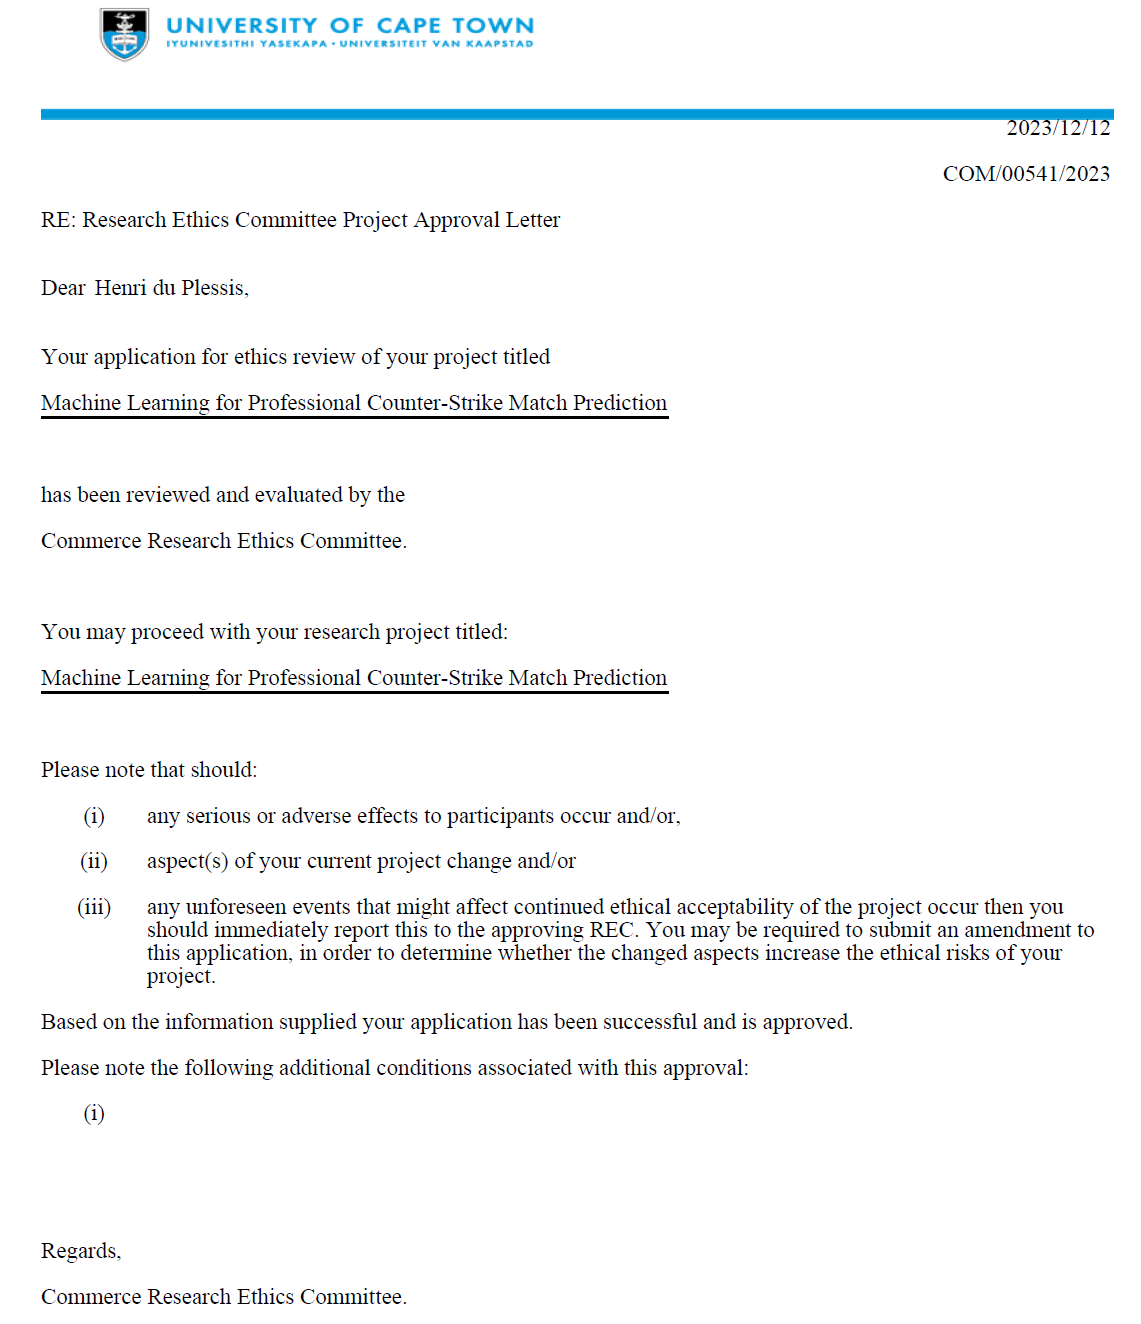
\includegraphics[width=1.1\textwidth]{Figures/ethics-approval.png}
	\end{adjustbox}
	\label{fig:ethics}
\end{figure}
%\include{Appendices/AppendixC}

%----------------------------------------------------------------------------------------
%	BIBLIOGRAPHY
%----------------------------------------------------------------------------------------

\printbibliography[heading=bibintoc]

%----------------------------------------------------------------------------------------

\end{document}  
